\documentclass[10pt,twocolumn]{article} % removed a4 option (is default)

\usepackage[margin=1.5cm]{geometry}
\usepackage{nameref}
\usepackage{hyperref}
\usepackage{titlesec}
\usepackage{graphicx}
\usepackage{enumitem}
\usepackage{xurl}
\usepackage{caption}


\setlength {\marginparwidth}{2cm}
\usepackage{todonotes}

% Set heading spacings, please don't change this
\titlespacing\section{0pt}{8pt plus 4pt minus 2pt}{0pt plus 2pt minus 2pt}
\titlespacing\subsection{0pt}{8pt plus 4pt minus 2pt}{0pt plus 2pt minus 2pt}
\titlespacing\subsubsection{0pt}{8pt plus 4pt minus 2pt}{0pt plus 2pt minus 2pt}

\author{
  Belinda Kneubühler (2504756K), Ben Hanmer (2505218H),\\
  Daniels Vasiljevs (2500414V), Shaun Loughery (2193422L),\\
  Zsuzsanna Szugyi (2418750S)}

\title{Puzzle Map}
\date{} % Leave empty

\setlength {\marginparwidth}{2cm}

\begin{document}

\maketitle


% ------------------------------------
\section*{Introduction}

This is the template for the MHCI coursework report.

% ------------------------------------
\section*{Purpose}

The main purpose of the product is to create an interactive, gamified mobile application for the discovery of the University campus that helps students and staff learn more about the University in an individual or group setting. It is developed to promote discovering the whole of the university in choosable paths and speeds,  and to encourage social activities as opposed to lone solutions. It is to be available for any current or prospective student and staff - all registered at the university with a GUID - , but the main target demographic are new students.\\
The system is based on a remote database which stores the details of the locations and users, and this data is served to the user in the form of a mobile device application, as this provides the best user experience (UX).

% ------------------------------------
\section*{System Description}

\subsection*{Functionality}
Users can access the app by creating an account using their university email (specifically, GUID). The app allows for not only the creation of the account, but the maintenance (forgotten password, change details, etc.), and deletion of it. Users have to fill out a personality quiz, the answers of which will later on bias the likelyhood of what location a user will most likely get offered to head to next. The app will make it possible to read an interactive checkpoint, e.g. AR tag, which would prompt a riddle to the user that they need to solve. In the possibility of the puzzle being too hard to decipher, there are 3 hints available for each, which make the puzzle gradually easier to solve. The app will also allow for users to increase their in-game experience by correctly solving riddles, and use the experience to level up and gain rewards by doing well in the app. The system also allows for and promotes social interactions between users, to work together to a shared goal of successfully solving a riddle.

Aspects that entertain and engage the user include the riddles/puzzles, AR and the checkpoints, achievements and online character development, friend connections and gifting, freebies and rewards to gain, and the learning of insider information about the campus.

\subsection*{User characteristics and needs}
The goals of the users would be to visit as many locations on campus as possible, and do it in the most efficient way gaining the most bonus from solving riddles correctly. This would give them increased chances to gain freebies, level up and develop their level of experience, which would keep them captivated, entertained and interested. New students and faculty would use the app to get more information about the campus, while existing university members would use the app to either learn about the university with a delay, or to put their existing knowledge to use to gain as many points as possible and get the rewards.

The main motivation, however, of any type of user is likely to be the love of mysteries, problem solving, and the possibility to pass the time in a fun way and interact with peers with a more relaxed environment than social media. In the case of any users, however, it can be assumed that they have a busy lifestyle and therefore the app is a series of short tasks without expiry dates, which can fit around any student/staff member's schedule.

\subsection*{Constraints}
The two biggest constraints to the operations of the app are the user's device capabilities, and the reliability of internet connectivity. These are both aspects the app needs to be designed for, to minimise the disruption these constraints would mean. Since users can walk freely around campus, gepgraphical and physical obstacles do not represent significant constraints.

\subsection*{Assumptions and dependencies}
The system and its operations can be affected by many external entities. This includes user device capabilities, the weather (if used when walking), developments in AR/MR technology, University redevelopment (buildings built/torn down, rooms made available/unavailable), and the user leaving the university having not completed the game yet.

\section*{Requirements}

\subsection*{Functional requirements}
The following are the main functional requirements the system has to fit:
\begin{itemize}[noitemsep]
  \item The system needs to scan the AR tag/QR code/etc.
  \item The system needs to randomly choose a building/riddle based on category
  \item The system needs to register category chosen
  \item The system needs to register personality test results
  \item The system needs to respond randomly with bias from personality test
  \item The system needs to register the riddle being solved/not solved
  \item The system needs to update user profile based on solved/not solved riddle
  \item The system needs to update user profile in relation to freebies, levels, achievements
  \item The system needs to handle account creation and logins
  \item The system needs to communicate with a database to store all data
  \item The system needs to communicate online
\end{itemize}

\subsection*{Non-functional requirements}
Non-functional requirements may not relate directly to the system's operations, but are equally important to consider for a good UX. It has been shown loading times affect the number of users retained by a service\footnote{\url{https://developers.google.com/web/fundamentals/performance/why-performance-matters}}. Therefore the following performance limits were set for the app, speedwise: the system should login in \textless5s, recognise tags in \textless5s, and complete the initialisation (show splash screen) in \textless20s.\\
It is also key to calculate for errors that might happen. To ensure users are never left in the dark, in case an unexpected issue were to happen, the system must show an error page with a clear message on what has happened, and what should be done by the user to mitigate it (e.g. "Uh-oh, something puzzled our app! Please leave feedback here \textless link\textgreater!".
\subsection*{Safety and Security}
While the design of the app focuses on most interactions happening when the user is stationary by a checkpoint, it allows for it to be used when the user is mobile (check map, friends status, etc.). To ensure the safety of the users, the app therefore does not require to be constantly watched. This is complemented by the non-linearity of the application, as the user can choose their own path, and therefore can avoid unsafe areas. The system also needs to be protected to avoid the loss of data, therefore the remote database requires regular backups - this can be supported by the user data being stored on the device locally.
\subsection*{Quality, maintainability and availability}
The quality of the product is the final aspect focused on. It was determined that not only the database and the app should be available at all times, but the checkpoints, too. These naturally vary based on building opening times, but the app has to provide satisfactory information on when checkpoints may not be available. The system also needs to correctly relay and register checkpoint location information, as well as be easily adjustable and maintainable for the adding and removal of checkpoints. 

% ------------------------------------
\section*{Concept Generation}
At this stage of the project, the 5 team members decided to come up with interaction ideas on their own, which was followed by a group discussion of the strengths and weaknesses of each idea.
It was agreed upon that we are to build an application that presents small puzzles or riddles to the user, who then has to solve them to get to certain locations on campus, but can do so in their own time, pace and order.
For this two key components were necessary to be defined: the details of checkpoints, and the riddles.
Each member created storyboards for these two interactions to see how our users, our system and the environment would behave with each other.
These were summarised and a set of example initial storyboards were created, which can be found in Appendix C.
\subsection*{Checkpoint Interactions}
The starting point was to determine how a user would check in at a checkpoint, as it is the most significant design component of the project. 
The theme of this interaction was fairly similar across the team, with all 5 team members considering using QR codes that need to be scanned. 
This was further supported by the team arguing that AR codes are very similar in construction, and expanding on the QR element idea to AR would provide a better user interaction. 
By having the user be able to interact with the checkpoint in 3D after scanning the code, we could add another gamified, interactive element to the action, making it more enjoyable. 
The ideas for AR items to be visualised included mascots, treasure chests, question marks, gift boxes and breakable items that need to be tapped several times to "break into" them and reveal the checkpoint achievements.

Other ideas considered for checkpoint interactions was using an RFID tag to mark the location. This would be possible, as most modern day mobile devices are all configured to use Near-Field Communications (NFC) technology. 
NFC is the basis of many smartphone application, most importantly mobile pay services, such as Google Pay, Apple Pay and Android Pay. Android users can use NFC for virtually any application, Apple users however can be restricted to only payment service uses, based on the model and Operating System they are running. 
This idea would have meant a need for custom made NFC tags to be placed at the locations, thus it was deemed a less ideal option due to the fact they are more costly to set up, and are harder to replace.

Overall, it was agreed that with any check-in, the phone should provide audio- and physical feedback by playing a small tune and vibrating - the type of sound and the length or number of vibrations can vary whether the location is correct or not.
\subsection*{Riddles}
The next interaction we focused on was the other selling point of our application: the riddles. 
It was decided that while it was necessary to make the puzzles accessible for everyone - with specific emphasis on international students visiting the campus, or even Glasgow for the very first time, - it was also important to keep riddles interesting.
This meant that the difficulty level of the riddles had to either cater for everyone, or to include different difficulty levels from which students choose from.
There were several varying ideas presented by the group members at this stage.
One idea was to provide different riddles in different languages, prompting users to seek out other users who speak that language, promoting the group aspect of the application. Some shortcomings regarding this idea were highlighted as modern day translation apps make it easy to "cheat", and that more introverted users may find this disheartening.
Other ideas included using poems such as haikus, sonnets or limericks, as well as wordplay type riddles, such as anagrams. It was agreed that these may be too difficult to solve for students who do not speak English as their first language.
The most widely agreed on idea was to simply describe the locations in plain English, hinting at certain physical or historical characteristics of each location. It was agreed that this would make the app the most inclusive, while at the same time presenting the user with information they may not already know.

Regardless of the riddle content, it was agreed the riddles can be selected by type (lecture, lab or social). For this, the screen will have to show three buttons to choose from. 
The placement of buttons varied by implementation, some pitching the idea of a classic 3 button list layout in the middle of the screen, and some prompting it should be included with a map.

The method of presentation of the riddles also differed in the ideas of team members. 
Those with the classic button layout either said the riddle should pop up as a generic notification, or the screen should change and an animation of a scroll "rolling out" should reveal the riddle.
Those who agreed the buttons should be embedded in a map screen, argued the riddle should not be presented as new screens, but rather overlay the map screen as popups or overlay as the animated scroll rolling out.
It was also pitched the riddle could reveal itself by slowly swimming down from the top of the screen, which received positive reviews from the team.
With either revelation method it was agreed that this is one of the gamification elements that can entertain users and make for great UX, therefore is important we get it right.

The team agreed on the user feedback regarding riddles as well, and settled that the riddle reveal should be accompanied by a sound effect (a "whoosh" shound for the scroll, or a "pop" sound for the popup) to make the app more interactive, and regardless of the placement of the buttons, they should provide both physical feedback (vibration when pressed) and audio feedback (tap sound when pressed), based on device settings configurations.
% ------------------------------------
\section*{Paper Prototyping}
Once the inital design ideas were agreed upon, the ideas could then be represented as paper prototypes. Each team member was reponsible with designing their own interaction prototypes that represents the previously agreed design choices.

Each team member presented their paper prototypes to the other team members. The paper prototypes were based on an imaginary story of a user on the app. The prototypes were reviewed by all team members. These paper prototypes are found in Appendix A.

\subsection*{Prototype 1}
The first prototype generated focusses on maintaining the map as the center of the user's view. The map will almost always be visible regardless of what the user wishes to do. The main interactive elements of the screen are located at the bottom of the screen. The only exception of this rule is that the settings button will be located at the top-left side of the screen.

The user can press the buttons at the bottom of the screen to navigate to the different sections of the screen. The user will always be within one or two screens away from the main map view. The buttons located at the bottom of the screen include: a home buton to return to the main map view; a button to view the current destination and available riddle; a button to initiate the camera module; a button to access a list of currently available offers and a button to access the profile.

\subsection*{Prototype 2}
Prototype two was split amongst more frames and was more focussed on keeping the screen from being cluttered. The user is greeted with a splash screen with a loading bar to show the current progress of loading the app. The user will then be guided to a signup/login screen. Once the user logs in for the first time, a quiz is displayed. This quiz will have questions and answers ranging from: strongly agree; agree; disagree and strongly disagree. Additionally, there will also be a progress indicator that shows the user how many questions are remaining. 

Once the user has finished the initial quiz, they will be given the option to select a riddle. Once the user selects a riddle, the question is displayed on the screen. The user can swipe left from this screen to access a list of available hints and unlock any other hints they require. The user can also swipe right and access the camera. This camera is used to take a picture of the AR code to complete the riddle. 

In addition to these screens, the user will also be able to access their profile. This will contain relative information about the user such as their username and profile picture. The user will always have a back button to escape back to the view containing the current riddle.

\subsection*{Prototype 3}
Paper prototype three is more focussed on user interactivity. When the user initially starts the application, they are greeted with a splash screen with the app logo. This splash screen converts into a login screen for the user. The users are also given an option to create an account.

Once the user logs into their account, they are shown the main screen of the app. This screen has a list of options for the user to select from. If it is the user's first time using the app, a button labelled "get started" which the user will be directed to find a valid AR tag. Otherwise, if the user has already initiated a riddle, they can access their current riddle from that screen. There is a "profile" button which can show the user their profile and all the achievements they have gained. Additionally, there is a "settings" button which takes the user to a page that has all the settings that can be modified to change the game mechanics.

When the user is asked to select a location, they are shown a screen which gives them three options: Lab; Lecture or social.

Once the user has selected a riddle, the riddle is shown on screen. The user has a set number of hints and as they use these hints, the riddle changes and becomes easier to solve. The user can then choose to solve the riddle at any point by swiping up from the bottom to open the camera. 

Once the user scans the AR code, the app will inform them if they have been successful and scanned the correct location. The app will also inform them if they have levelled up and any free offers they have unlocked.

\subsection*{Prototype 4}
This prototype also focussed heavily on maintaining a minimilistic design. This prototype uses many different screens to display information. 

The prototype has an initial start screen with a button to continue to the login screen. This login screen has an option to remember the user. Once the user logs in, if this is their first time using the app, they are displayed with a personality quiz. Otherwise, the main screen is shown.

The main screen consists of the main map view and the logo of the app. This screen also hosts a floating action button that can be used to open the camera module. If the user opens the camera, a basic AR scanner is shown on screen. 

Once a user scans a valid AR tag, they are shown with a screen that details information about the area and informs the user about the amount of XP they have gained. The user can then press a button to continue and the app will give them four buttons that can be selected to direct where they want to go. Once the user has selected a location, the main screen will show again and the riddle for the new location will be shown on screen overlaying the map.

The profile can be accessed through the settings menu. This profile will display: the user's name; the user's profile picture; the basic information held about the user; the user's friend list and a back button to return to the main map screen.

\subsection*{Prototype 5}

The final prototype suggested had a similar structure to the previous prototypes. A minimalistic design was implemented for the initial use of the app. The user would be greeted with two buttons; one to sign up and one to log in. When the user has signed in for the first time they will be greeted with a quiz.

After they complete this quiz, they will be greeted with the main view of the app. This consists of a main map view with several buttons at the top and bottom of the screen. The buttons at the top of the screen will give the user the option to select a lab, lecture or social based riddle. The user will not be limited to one riddle at a time to allow them to revisit riddles that they can not currently solve. The key points will be highlighted on the map as starts.

The bottom part of the screen will swipe up to reveal a navigation drawer. This drawer will contain buttons that can be used to navigate to the other parts of the application. For example, a hints button will give them tips for the current riddle. A camera button will be visible which allows the user to scan an AR code. This AR code will signify the user completing the riddle. Additionally, if the user scans an incorrect AR code, they will be given the option to claim the reward anyway or leave and come back. Another button could be visible which shows the user their currently available offers. The user will also be able to access their profile from this navigation bar. Their profile will show their name, icon and their current skill levels.

\subsection*{Testing the Prototypes}
Each of these paper prototypes were evaluated within the team. These ideas were discussed and the good and the bad interactions were noted for the refined prototype.

When the application opens, it should show a splash screen. Various interactions were suggested such as a screen that requires a button or finger press to go away. It was decided, however, that a splash screen should be shown that disappears after a few seconds. This allows the user to see that they have entered the right application, but not intrude the users view of the app.

When the application has started, the user will be presented with a login screen. This screen will have a button to log-in to an existing user account or sign-up with a new account. This screen should remain fairly simple, with perhaps only the logo of the application and the application name in addition to this.

The map should be the main focus of the screen. The user should always be able to see where they are in location to a map screen. If other screens were needed to convey information, the user should always be able to easily return to the base map screen.

Swipe motions that were near the edges of the screen were avoided. This is because new smart phones use gesture based navigation. Users would accidentally use the gesture based navigation of their smart phone instead of the application.

A overall goal of the application is to not discourage users from continuing to use the app. If the user had went to the wrong location, they should still be rewarded for exploring, but informed that they have reached the wrong destination.

The application should encourage individual users to use the application with their friends. Several features to encourage this include the ability to add friends via a QR code. Riddles can be included that require the QR code of another user to be scanned. Random gifts could be given that can only be sent to friends.

It is important that the user is not frustrated when they are unable to solve a riddle and can not get stuck in the same position. Ideas to counteract this include: providing various different riddles that can be swapped between at the same time; providing hints to the user that will eventually give the direct path to the intended destination and providing the user with the ability to scan AR codes without knowing the associated riddle (incase they accidentally scan the wrong code). Additionally, if the user does scan the wrong associated code, they should be given the option to 'cancel' their decision so that they can try to find the right code again.

This generalised feedback can be summarised into the following list of good and bad points generated from the evaluation.

\subsubsection*{Good}
\begin{itemize}[noitemsep]
  \item Keep the design simple
  \item Allow the user to always be able to access the main map
  \item Keep a navigation bar accessable at the bottom of the screen with intuitive buttons
  \item Give the user access to always visit locations regardless of their current riddle state
  \item Reward the user for visiting locations regardless if they solved the riddle or note
  \item Provide a motive to the user to solve the riddles, such as extra experience points
  \item Provide the user with several riddles so that they are not stuck on one specific riddle
  \item Keep the splash screen minimal and make it automatically disappear rather than remain persistent
  \item Provide features that encourage making new friends
  \item Provide offers to the user to encourage them to keep using the application
  \item Give the user the option on what to do next after they solve the riddle
\end{itemize}

\subsubsection*{Bad}
\begin{itemize}[noitemsep]
  \item A map must be provided
  \item Do not use swiping motions close to the edges of the screens due to gestures built within the smart phone systems
  \item Do not use an excessive amount of on screen elements as this may confuse the user
  \item Do not provide only one riddle
  \item Having the settings menu as a persistent button clutters the screen and can be relocated elsewhere
  \item Do not punish the user heavily for not solving the riddle
  \item If the user accidentally answers the riddle incorrectly, do not trap them and give them the option to "cancel" their scan
  \item Do not make the initial quiz too detailed as this may confuse users
  \item Do not create too many layers of sub-menus that would cause the user to get "lost"
\end{itemize}

% ------------------------------------
\section*{Refined Prototyping}

Feedback was evaluated from the initial prototypes and a final version was created that combines the best parts of all of the previous prototypes.
As a base, the prototype \#5 was used, but updated with the learnings from all previous prototypes. The paper prototype is available for reference in Appendix B.

\subsection*{Changes from Previous Prototyping Stage}
Following are the main changes that were made to the last prototype (\#5): \\

The buttons for general interaction are kept on the bottom, but stationary. They are arranged so the camera icon is towards the middle and the profile is all the way to the right (the least important). As a first icon, a home screen icon (map) is added. Additionally, an offers button (the gift) is added. \\

On the top of the screen, the different riddle icons are shown next to the classic menu icon (burger menu). The riddles are displayed as a scroll that can be rolled up (swiped) or down to hide or display hints. Hints are displayed in text format; no arrows or direct navigation is shown.\\
Points of interest are highlighted on the map. They can be clicked, which will then display more information about the places.\\
There should be an option to add friends with a QR code (scanable with the camera) or by entering a user name. 

\subsection*{Implementation and Evaluation Clickable Prototype}
This prototype was drawn up again and made interactive with the Marvel App. It which has very similar features as Invision, which was introduced in the lectures. The advantage of Marvel is that it allows an unlimited number of prototypes in the free version. Both programs allow the designer to implement interactions on drawings that can be made directly in the program or on pictures. The later was used.


\subsection*{User Testing}

This clickable prototype was then sent to various testers through a link. They were then able to click through the displayed webpage like an app. Every tester was briefed initially about the general concept of the app and subsequently filmed while they were interacting with it. They were asked to comment on what they are seeing and doing and the designer, who was filming this process, gave them pointers on what to do or helped them if they got stuck, especially if that was due to limitations of the clickable prototype.

\todo{belinda, write some more}

\subsection*{Implications for Next Stage}
The following recommendations were identified during the user test:
\begin{itemize}[noitemsep]
  \item If no riddle is selected, a message should be shown below the buttons: "click to get your first riddle".
  \item The information pop-up about point of interest should still allow all other interactions and not have to be clicked away first.  
  \item More information about a point of interest should be displayed. (Trivia, where are the toilets or water fountains?)
  \item Have both swipe and click option in the offers to navigate from one QR-code to another.
  \item Remove the menu button. It is not needed an a settings menu can easily be stored away in the profile. This also increases the available space for the top buttons.  
  \item Hints need to be added when in scan mode ("ready to scan tag" / "click to activate").
  \item Hints need to be added to the riddles ("scroll down to get a hint", "scroll up to hide"), or at least arrows that point in the direction. Possibly allow click to reveal a new hint. If the user clicks anywhere on the map, that should hide the riddle.
  \item A prompt, like "are you sure you want to use a hint", should avoid accidentally using a hint for a riddle.
  \item Badges seem to be a good way to keep things interesting, people want to uncover the missing badges, the discovered ones should have some explanation, when clicked on ("discovered 5 cafés").
- add explations to badges (show them as pop-ups when clicking on them, display name, e.g. )
  \item An indication is needed for which navigation button at the bottom is active. (Selected register card.)
  \item Scanning a "wrong" solution should have more information. For example: "you get more points if you find this place with a riddle".
\end{itemize}
Additionally, some potential improvements have been identified that need to be explored further:
\begin{itemize}[noitemsep]
  \item Add the ability to see friends profile in more detail.
  \item Add more interaction with friends, like joint riddles or the ability to send gifts to friends.
  \item Show the riddle if the place is claimed without a riddle "just for the fun of it".
  \item Show the solved riddles in the map screen when clicking on the stars.
  \item Is AR really necessary? It certainly is a nice gimmick, but not specifically needed, scanning a code seems to be enough for the functionality.
\end{itemize}
% ------------------------------------
\section*{Demonstrator Prototype}

After recieving feedback from the refined prototype, a demonstrator prototype was created to show the implementation of the main design features within an application. This demonstrator prototype is created for Android devices and is created using "Android Studio". The application is created using Java. The application was developed for Android 9/Pie (API level 28).

This demonstrator prototype was developed by incorporating the feedback received from the previous prototypes. This prototype will give users a more realistic interpretation of what the final application will look like. This demonstrator prototype is not intended to be a final product, but will feature the main interactions, features and general design that the application will have.

It is important to note that, while many of the main features of the application remain, the structure and style of the app has developed significantly. This means that the initial storyboards (located in Appendix C) have also changed. The new updated storyboards can be found in Appendix D. 
\subsection*{Navigating The Prototype}
When the user first launches the application, they are greeted with a splash screen. This splash screen disappears and a log-in screen is displayed. Once the user logs in, they are greeted with the main view of the app.

The main view of the app contains a central map. There are three buttons located at the top of the screen: "Lab"; "Lecture" and "Social". This is accompanied by four icons at the bottom: "Home";  "Scan"; "Offers" and "Account". Clicking one of the three buttons at the top of the screen will scroll down a riddle associated with that button.

Clicking on the "Scan" button will open up a fullscreen scanner. If they scan the right code, they will recieve a pop-up congratulating them and will let them claim their prize. If they scan a valid code which is not the answer to the riddle, the pop-up informs them of this and offers them to leave the reward and come back when they have the associated riddle active.

Opening the offers screen shows the user the current offers they have unlocked, such as a free coffee. The user can swipe the screen left and right to swap between available offers.

If the user selects the account option, they will be shown their user profile. This screen includes the username and profile picture of the user. The current level of the user is displayed and a progress bar for their XP can be seen. There are four buttons on this screen: "Friends"; "Badges"; "Settings" and "Logout".

Clicking "Friends" shows a list of all of the friends a user has added. Their levels, names and icons are displayed. The user also has an option to add new friends with a button. Clicking the "Badges" button will show the user a list of badges they have unlocked. If the user clicks a specific badge, it will display more information about the badge in a pop-up notification. Clicking "Logout" will return the user to the log-in screen.

\subsection*{User Testing}
This demonstrator prototype was implemented into an Android application. This app was installed on several mobile devices which were given to individual users to evaluate their experience. A "think aloud" approach was taken and feedback was extracted from their experiences.

\subsection*{Evaluating the Demonstrator Prototype}
The following feedback was received from the demonstrator prototype:
\begin{itemize}[noitemsep]
 \item The purpose of the riddles is not obvious 
 \item The buttons are not self-explanatory and it is not obvious what their purposes are
 \item When a riddle is open, pressing the associated button does not close it and it can be confusing to remember which riddle is active
 \item It is not explained clearly as to where your rewards have went
 \item After clicking on a point of interest, reeclicking on the same point of interest does nothing
 \item It is not obvious as to how to use the scrolling interactions such as those for hiding the riddles and accessing hints
\end{itemize}

It is recomended then that, based on the provided feedback, if this application was to be developed into a final product, the following improvements should be made in a future revision:
\begin{itemize}[noitemsep]
 \item Create some sort of step-by-step tutorials explaining the purpose of the app and how to use its features such as the riddles
 \item Explain to the user the purpose of each button and their purpose
 \item Create some sort of feedback as to what riddle is currently visible - perhaps changing the colour of the button or pressing the button again hides the riddle
 \item Improve the clarity in the explanations for where earned rewards go and how to use them
 \item Clicking on the same point of interest should hide the description, and perhaps the currently selected point of interest should be highlighted in some way, such as changing it's colour
 \item Perform better feedback as to when certain items are scrollable - perhaps icons can be added that are used to identify scrollable objects, or provide a tutorial explanation
\end{itemize}
\section*{Conclusion}

\onecolumn
\section*{Appendices}
\subsection*{Appendix A - Initial Prototypes}
\subsection*{Prototype 1}
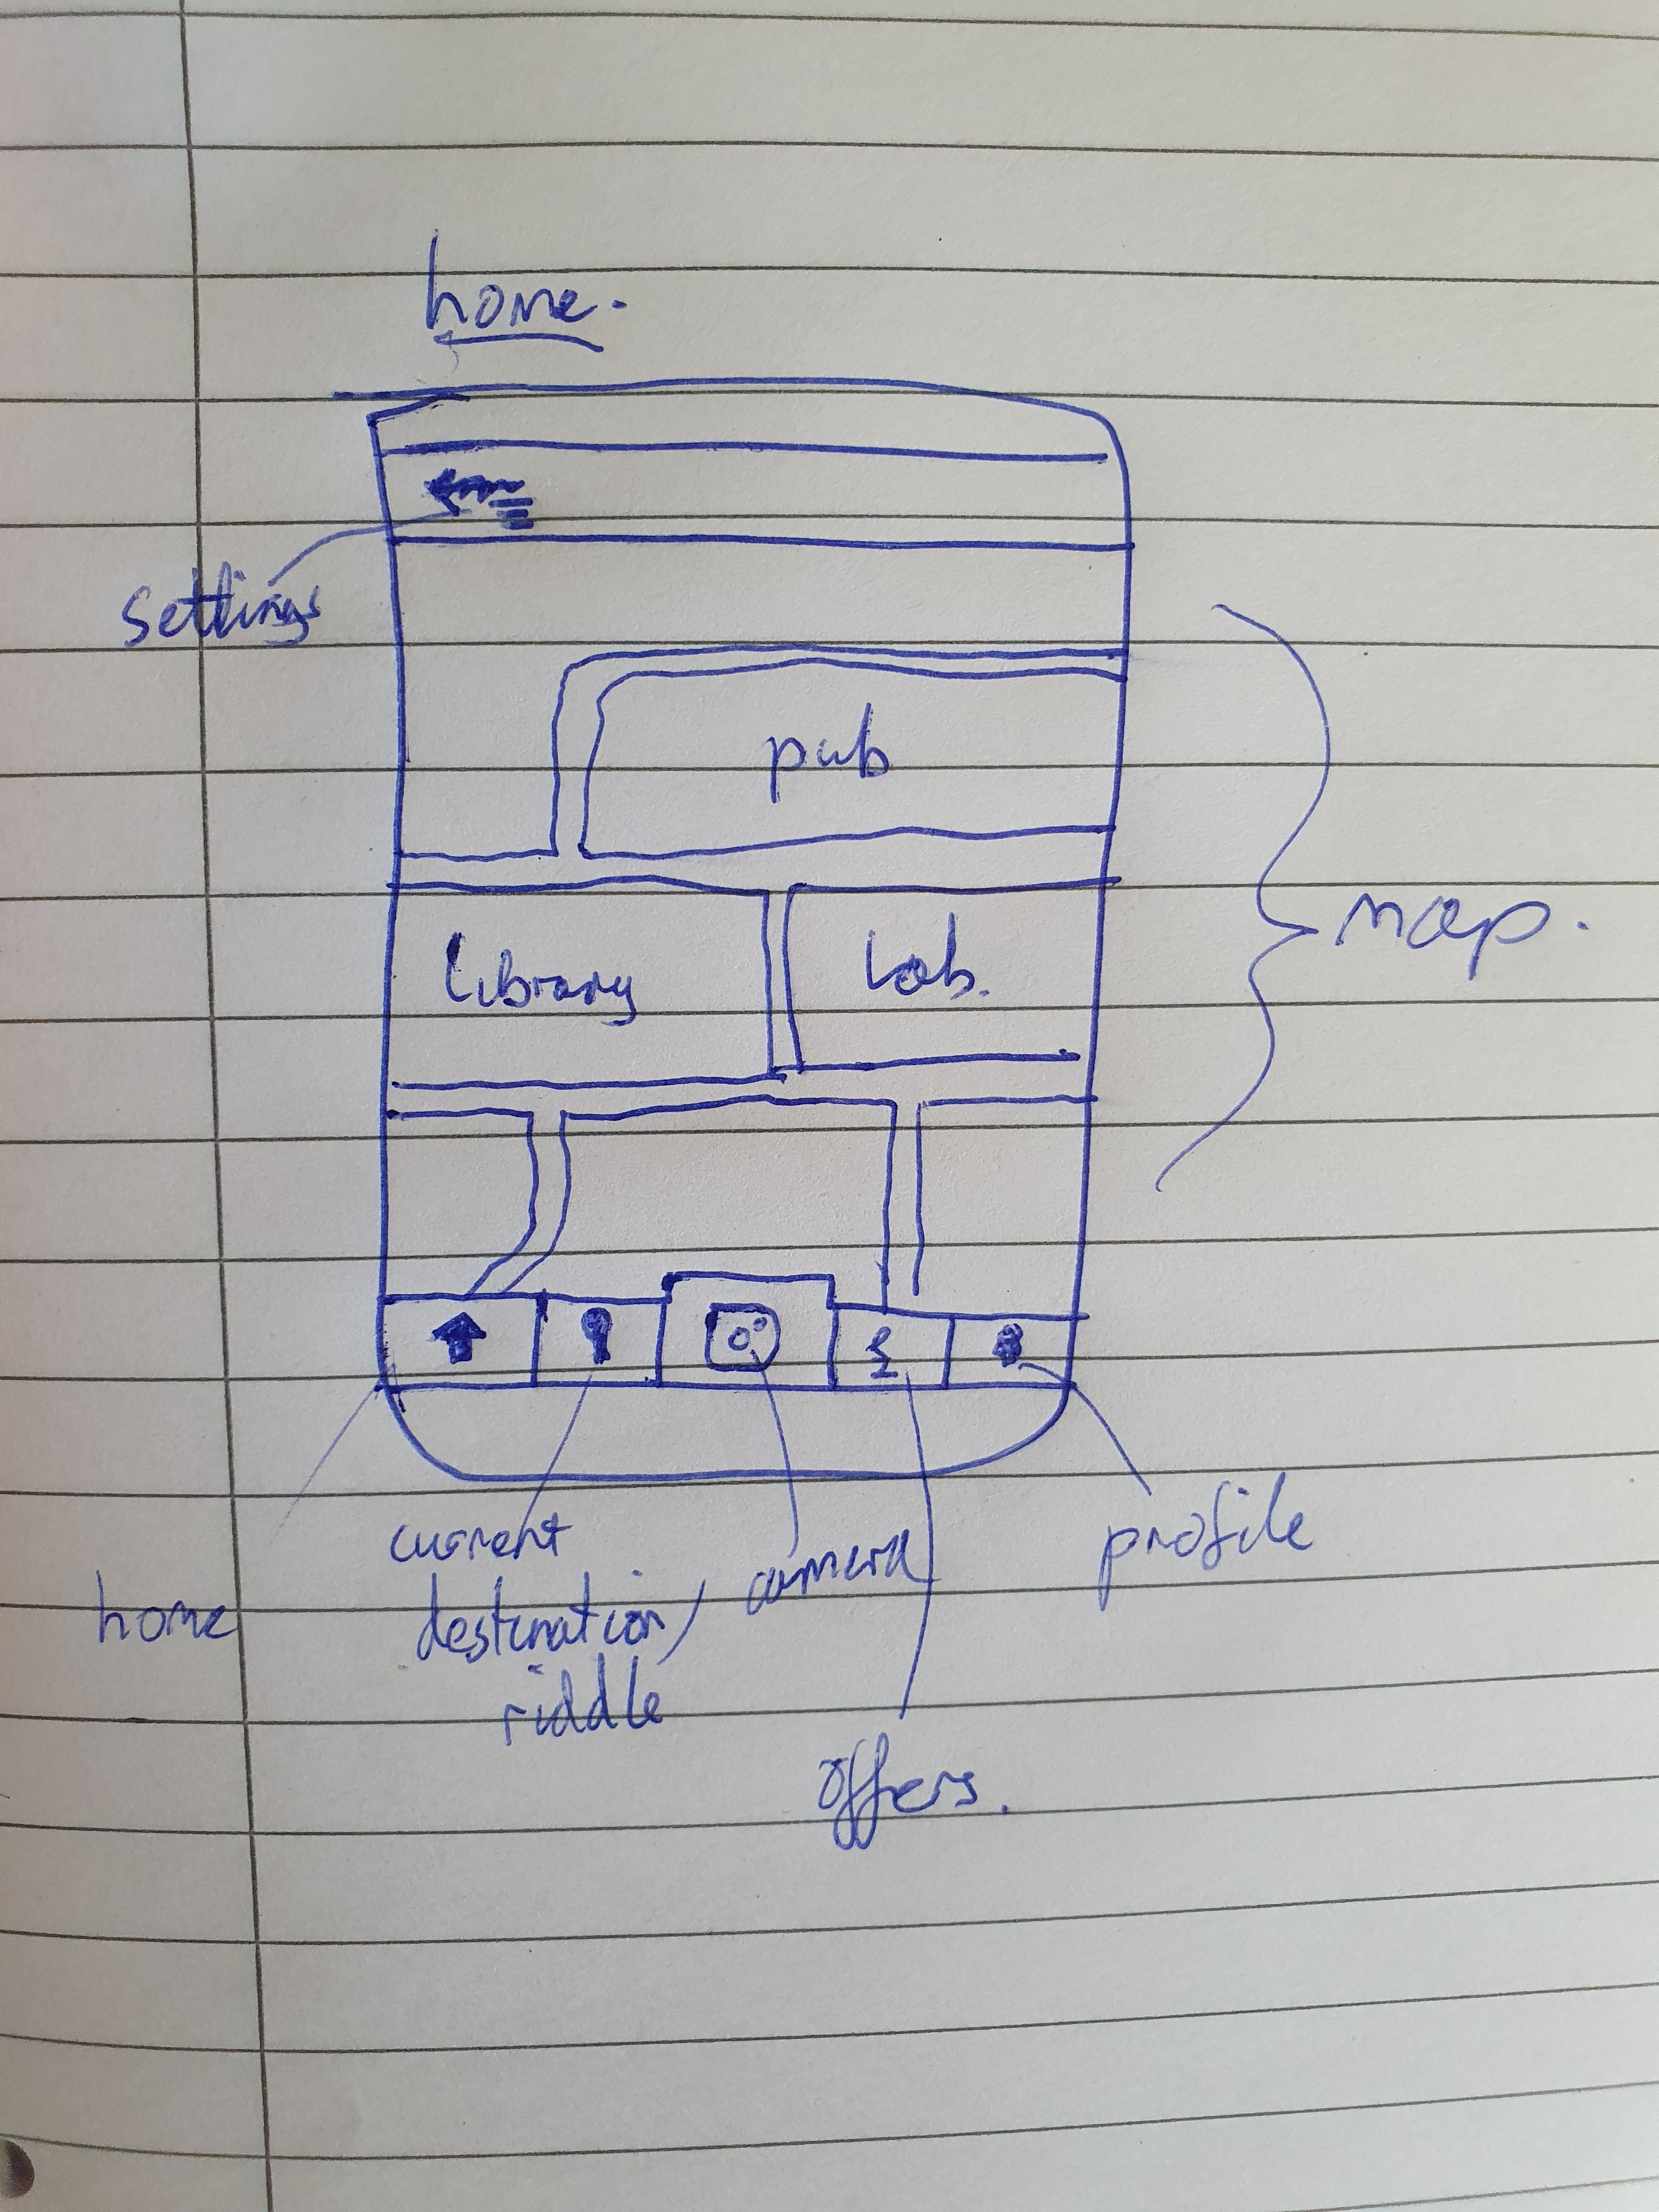
\includegraphics[width=0.5\textwidth]{./figures/bens_initial_proto/1.jpg}

\subsection*{Prototype 2}
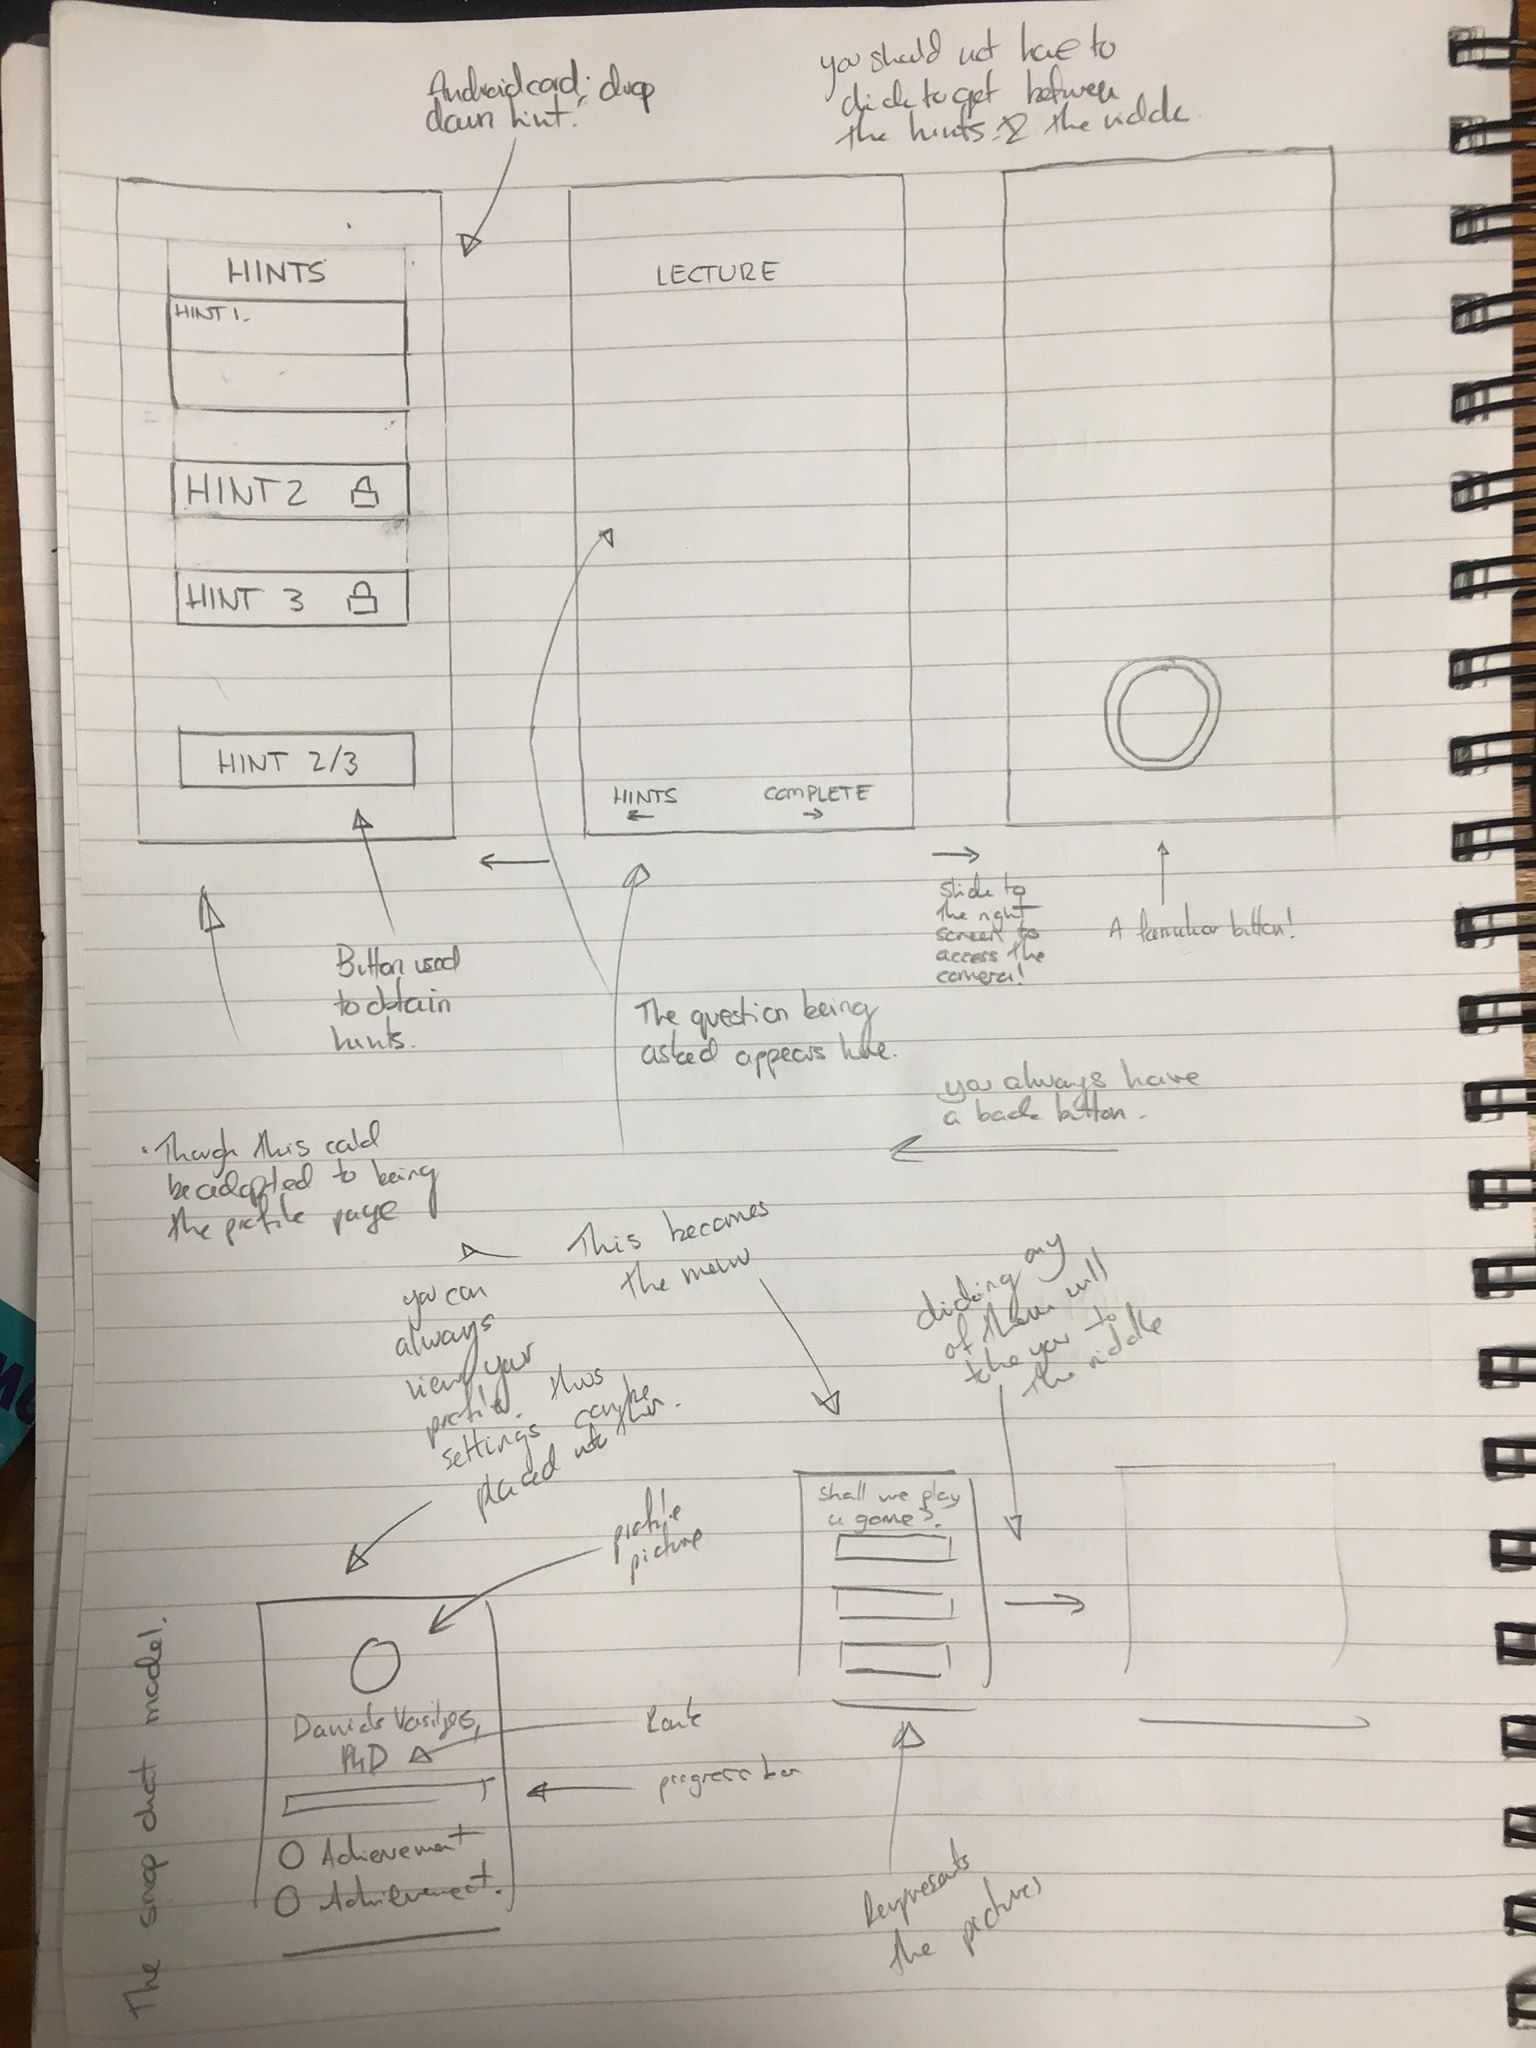
\includegraphics[width=0.5\textwidth]{./figures/dans_initial_proto/1.jpg}

\subsection*{Prototype 3}
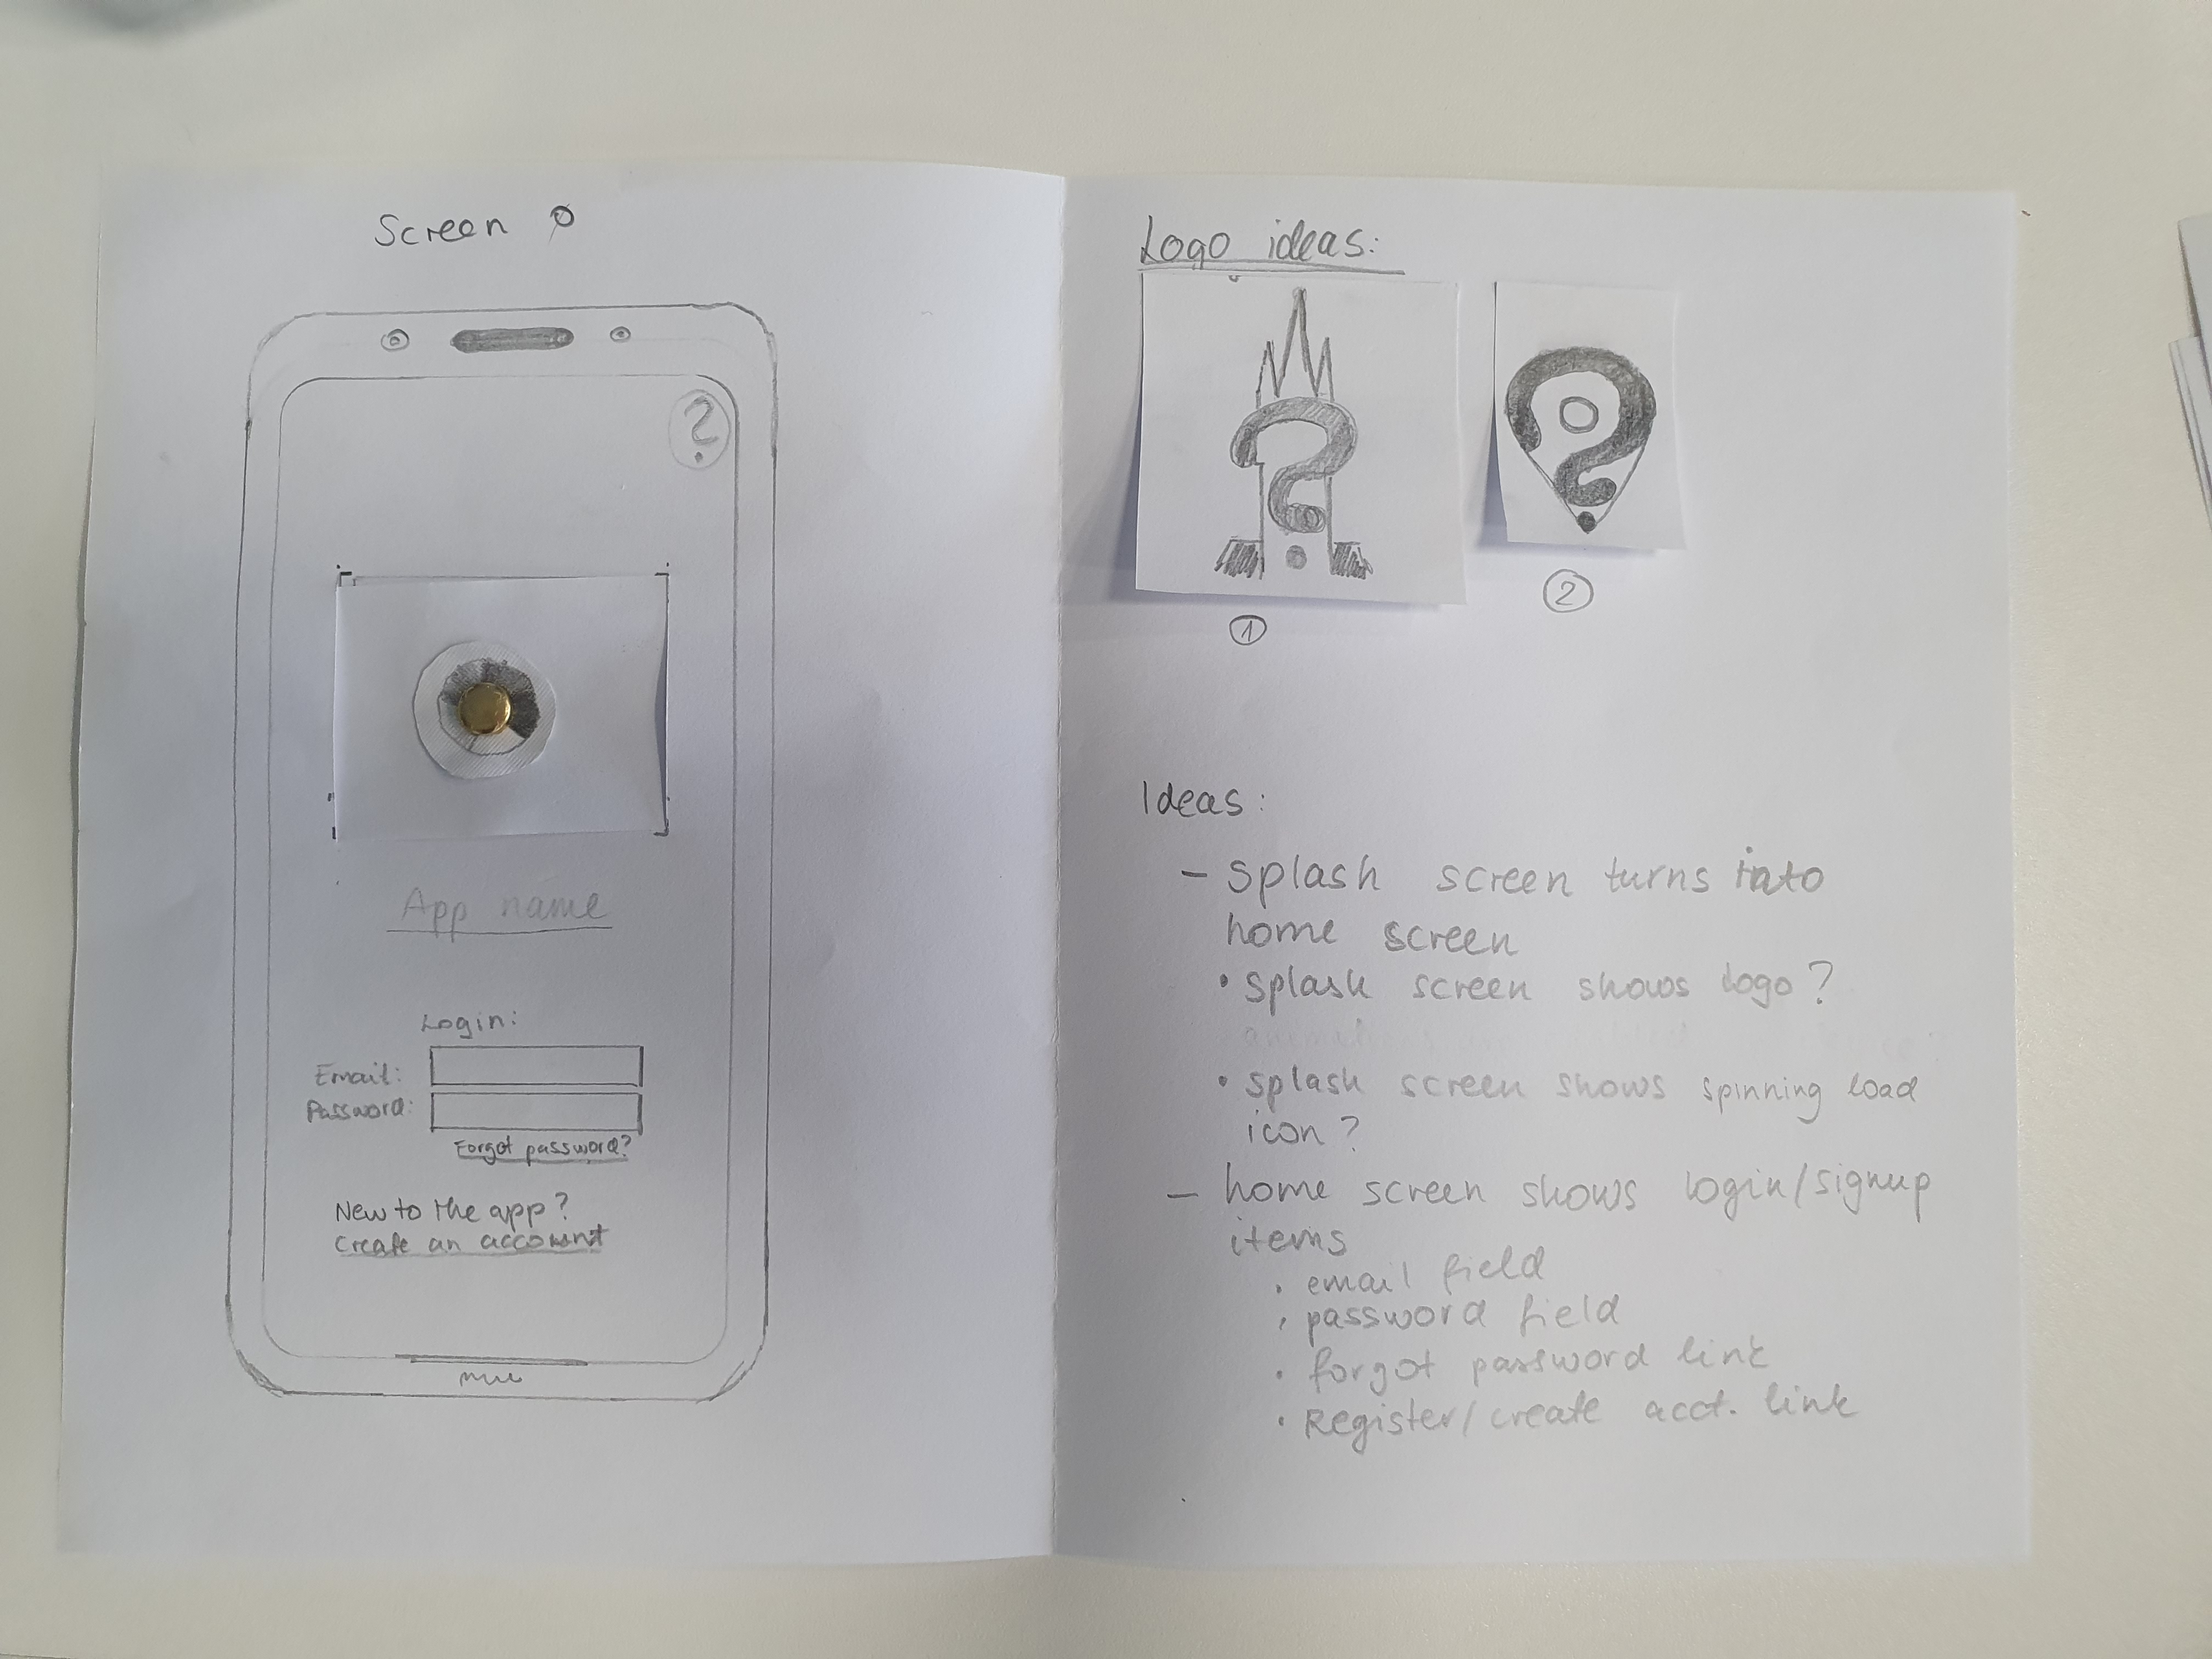
\includegraphics[width=0.5\textwidth]{./figures/zsuzsis_initial_proto/1.jpg}

\subsection*{Prototype 4}
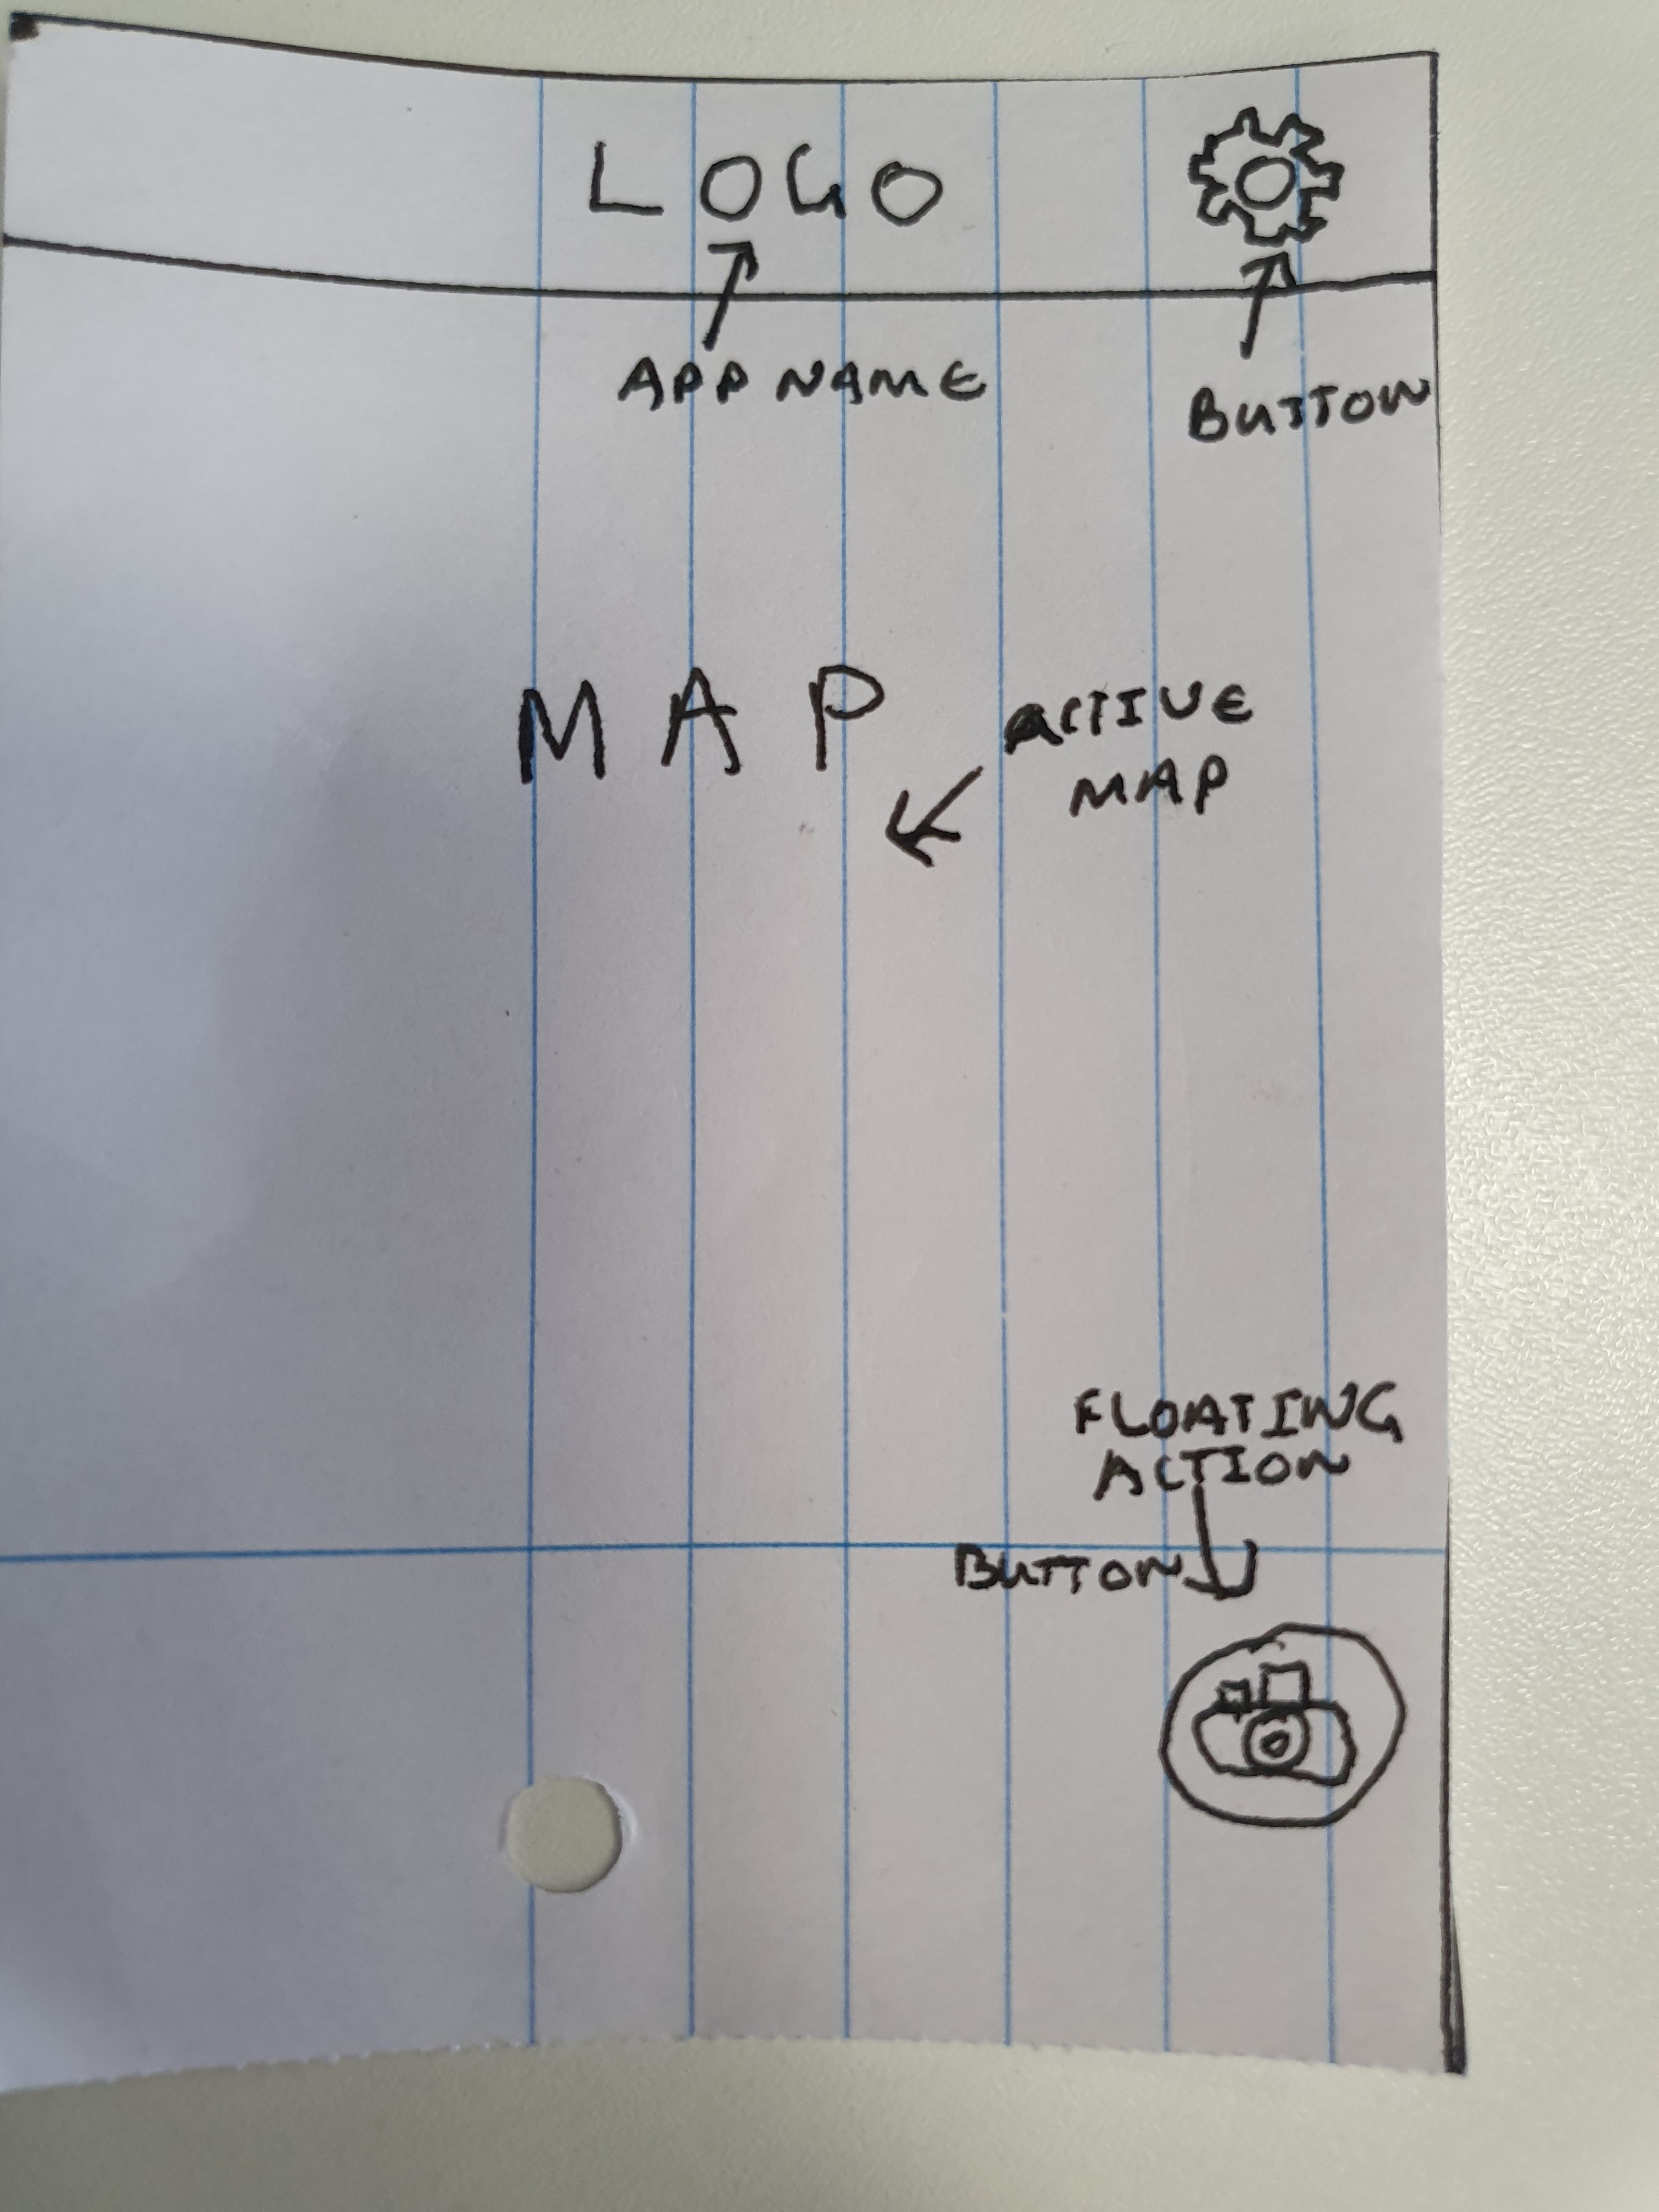
\includegraphics[width=0.5\textwidth]{./figures/shauns_initial_proto/1.jpg}

\subsection*{Prototype 5}
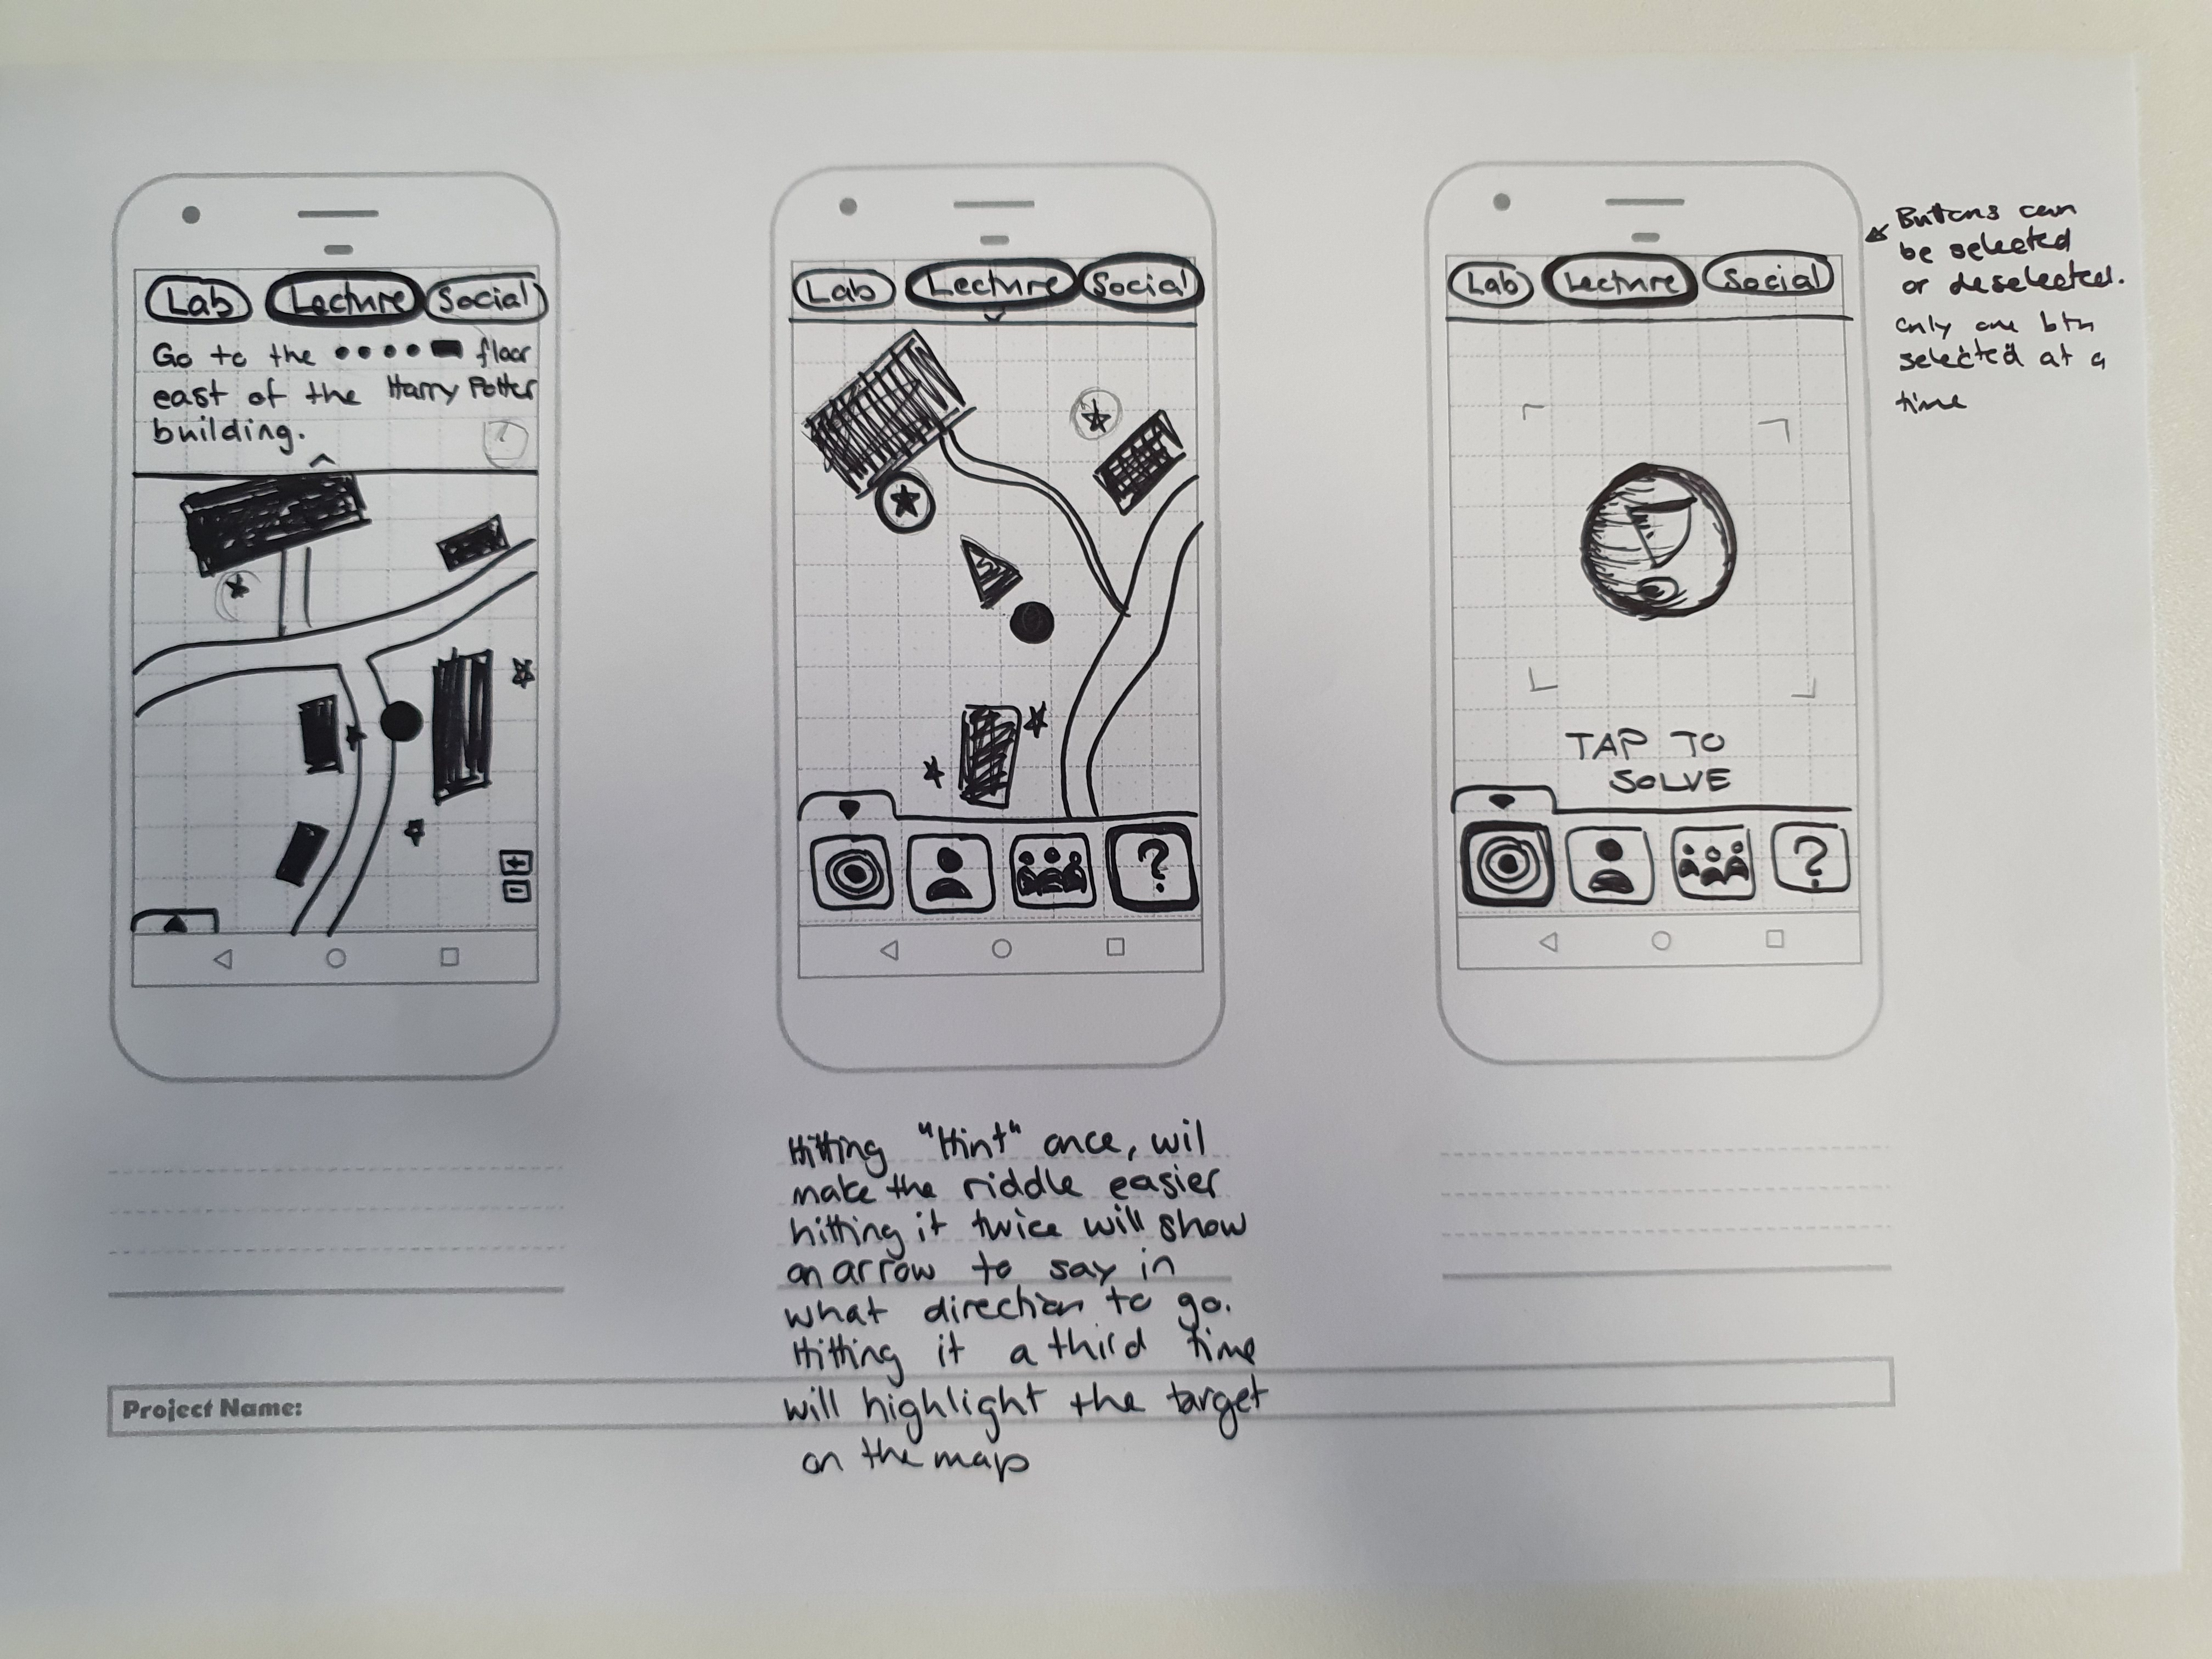
\includegraphics[width=0.5\textwidth]{./figures/belindas_initial_proto/1.jpg}

\newpage
\subsection*{Appendix B - Refined Prototype}
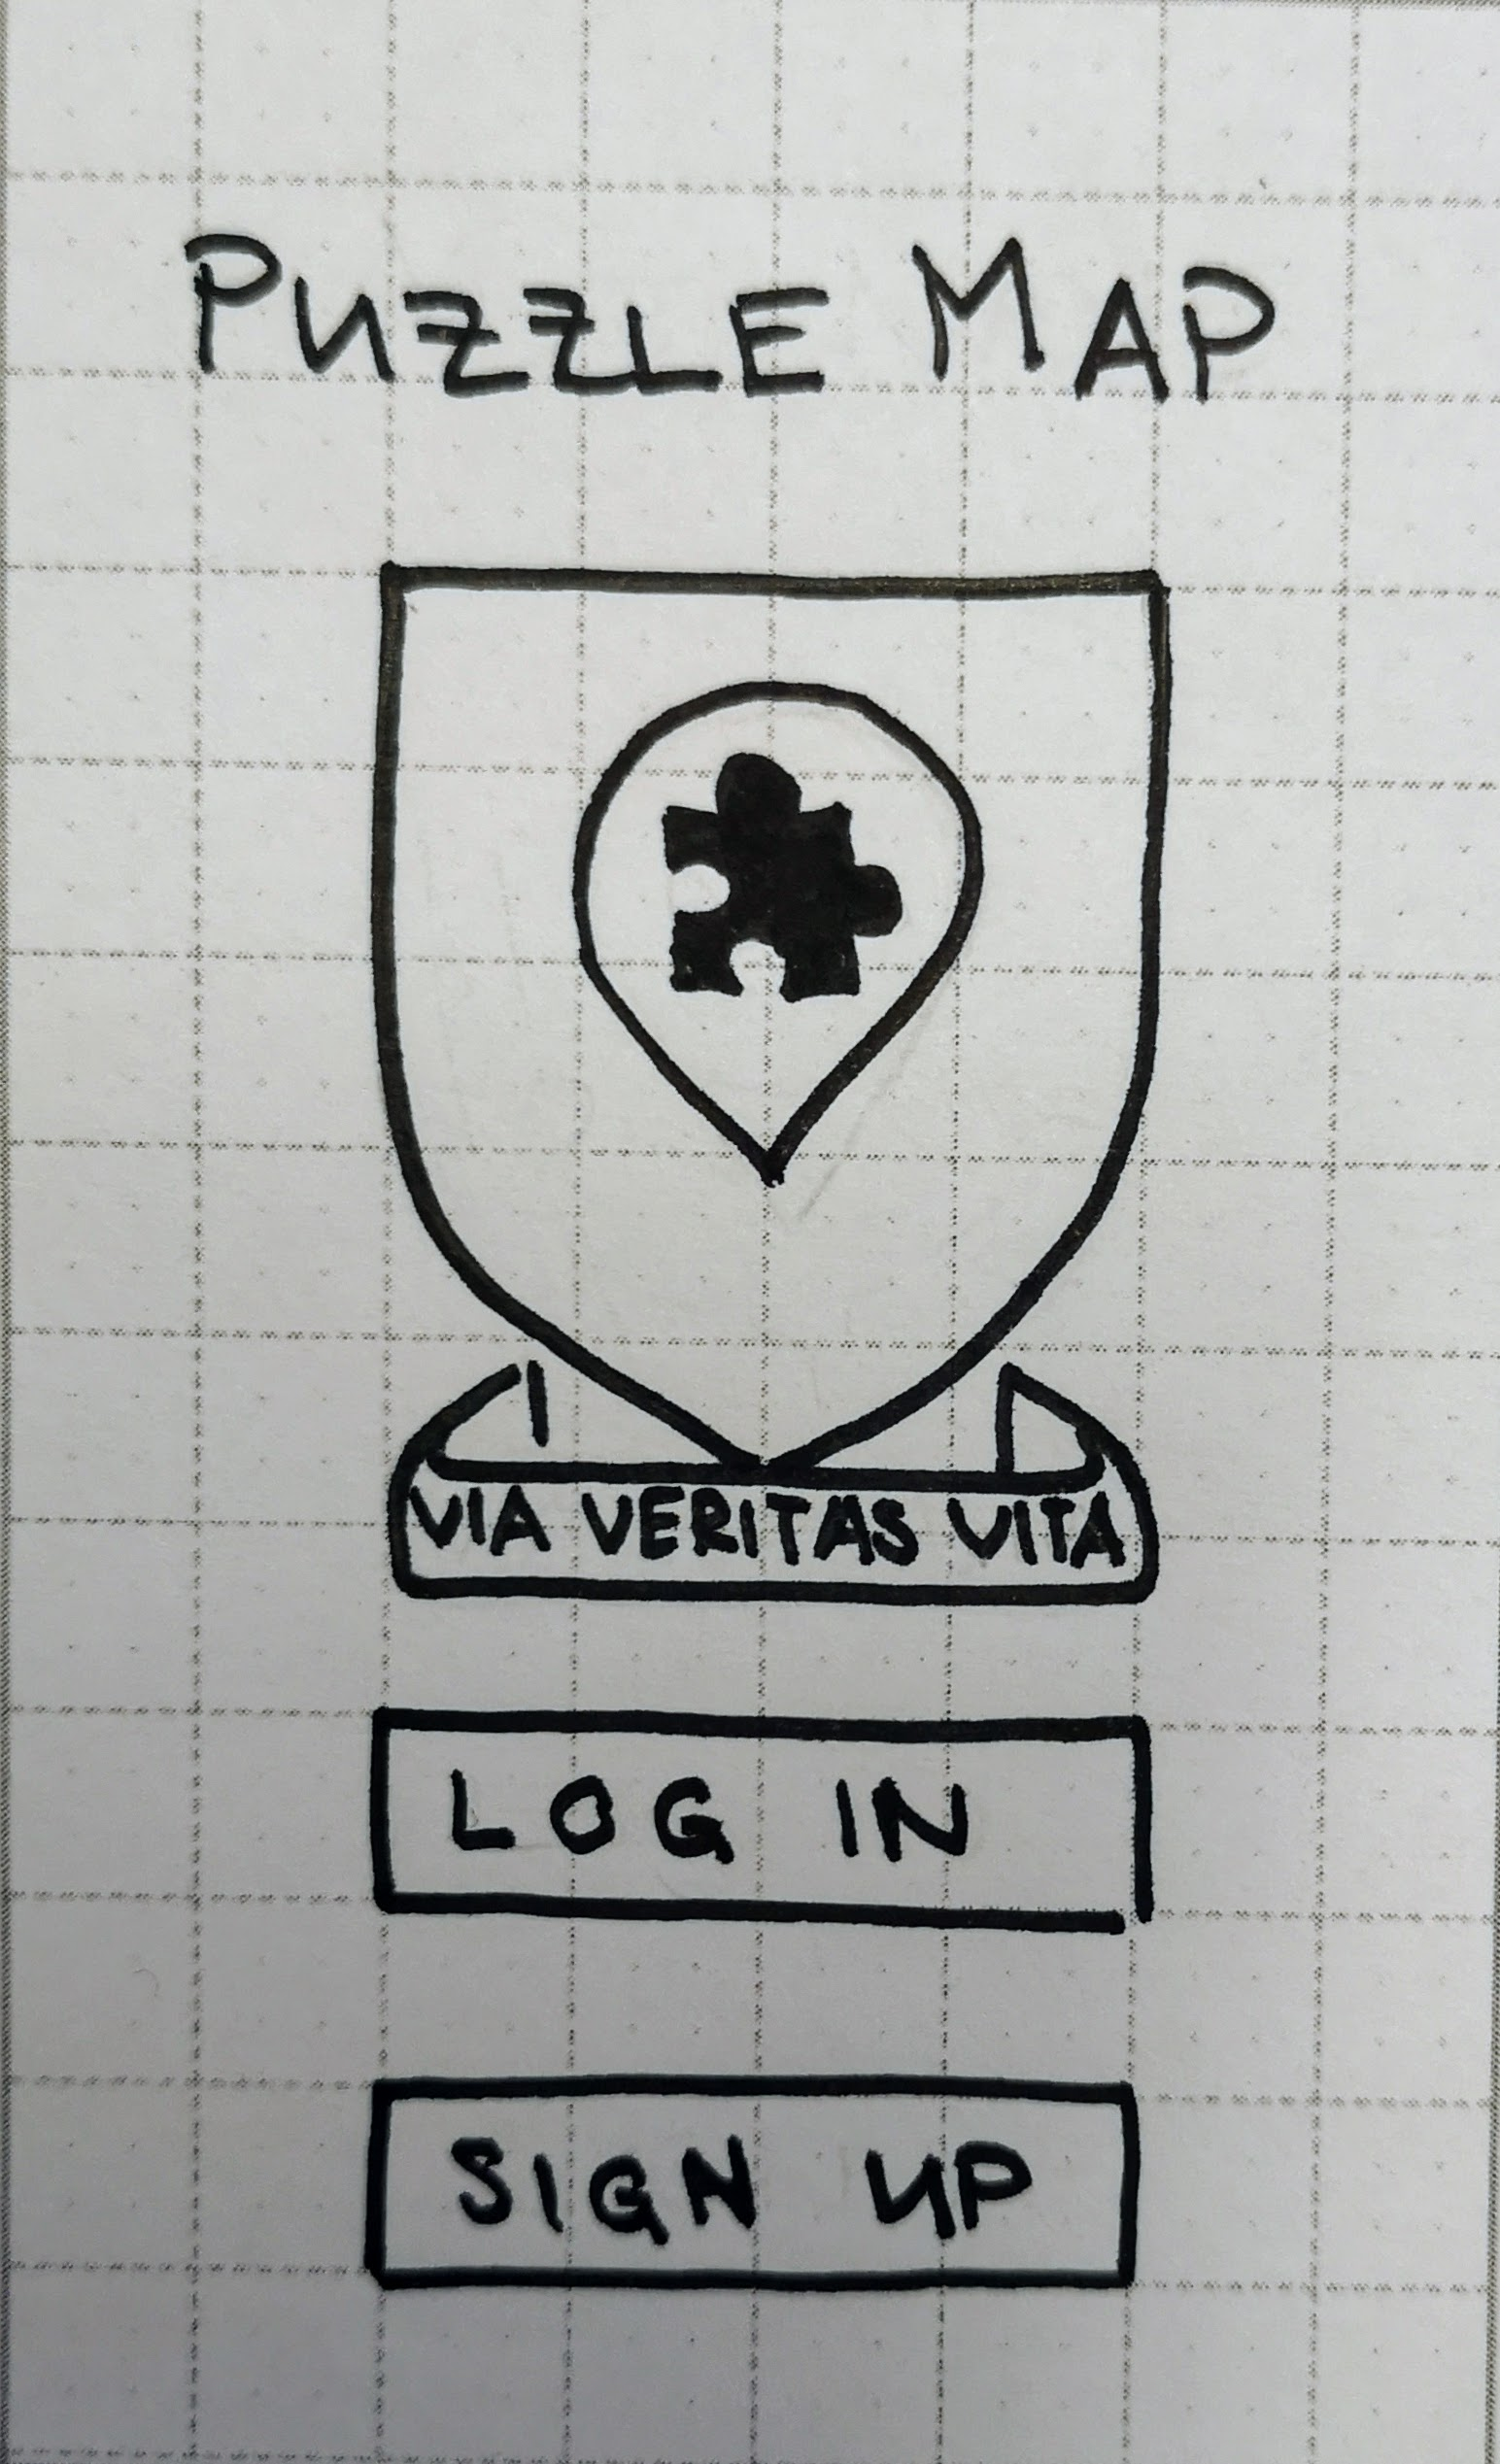
\includegraphics[width=0.3\textwidth]{./figures/refined_proto/1.jpg}
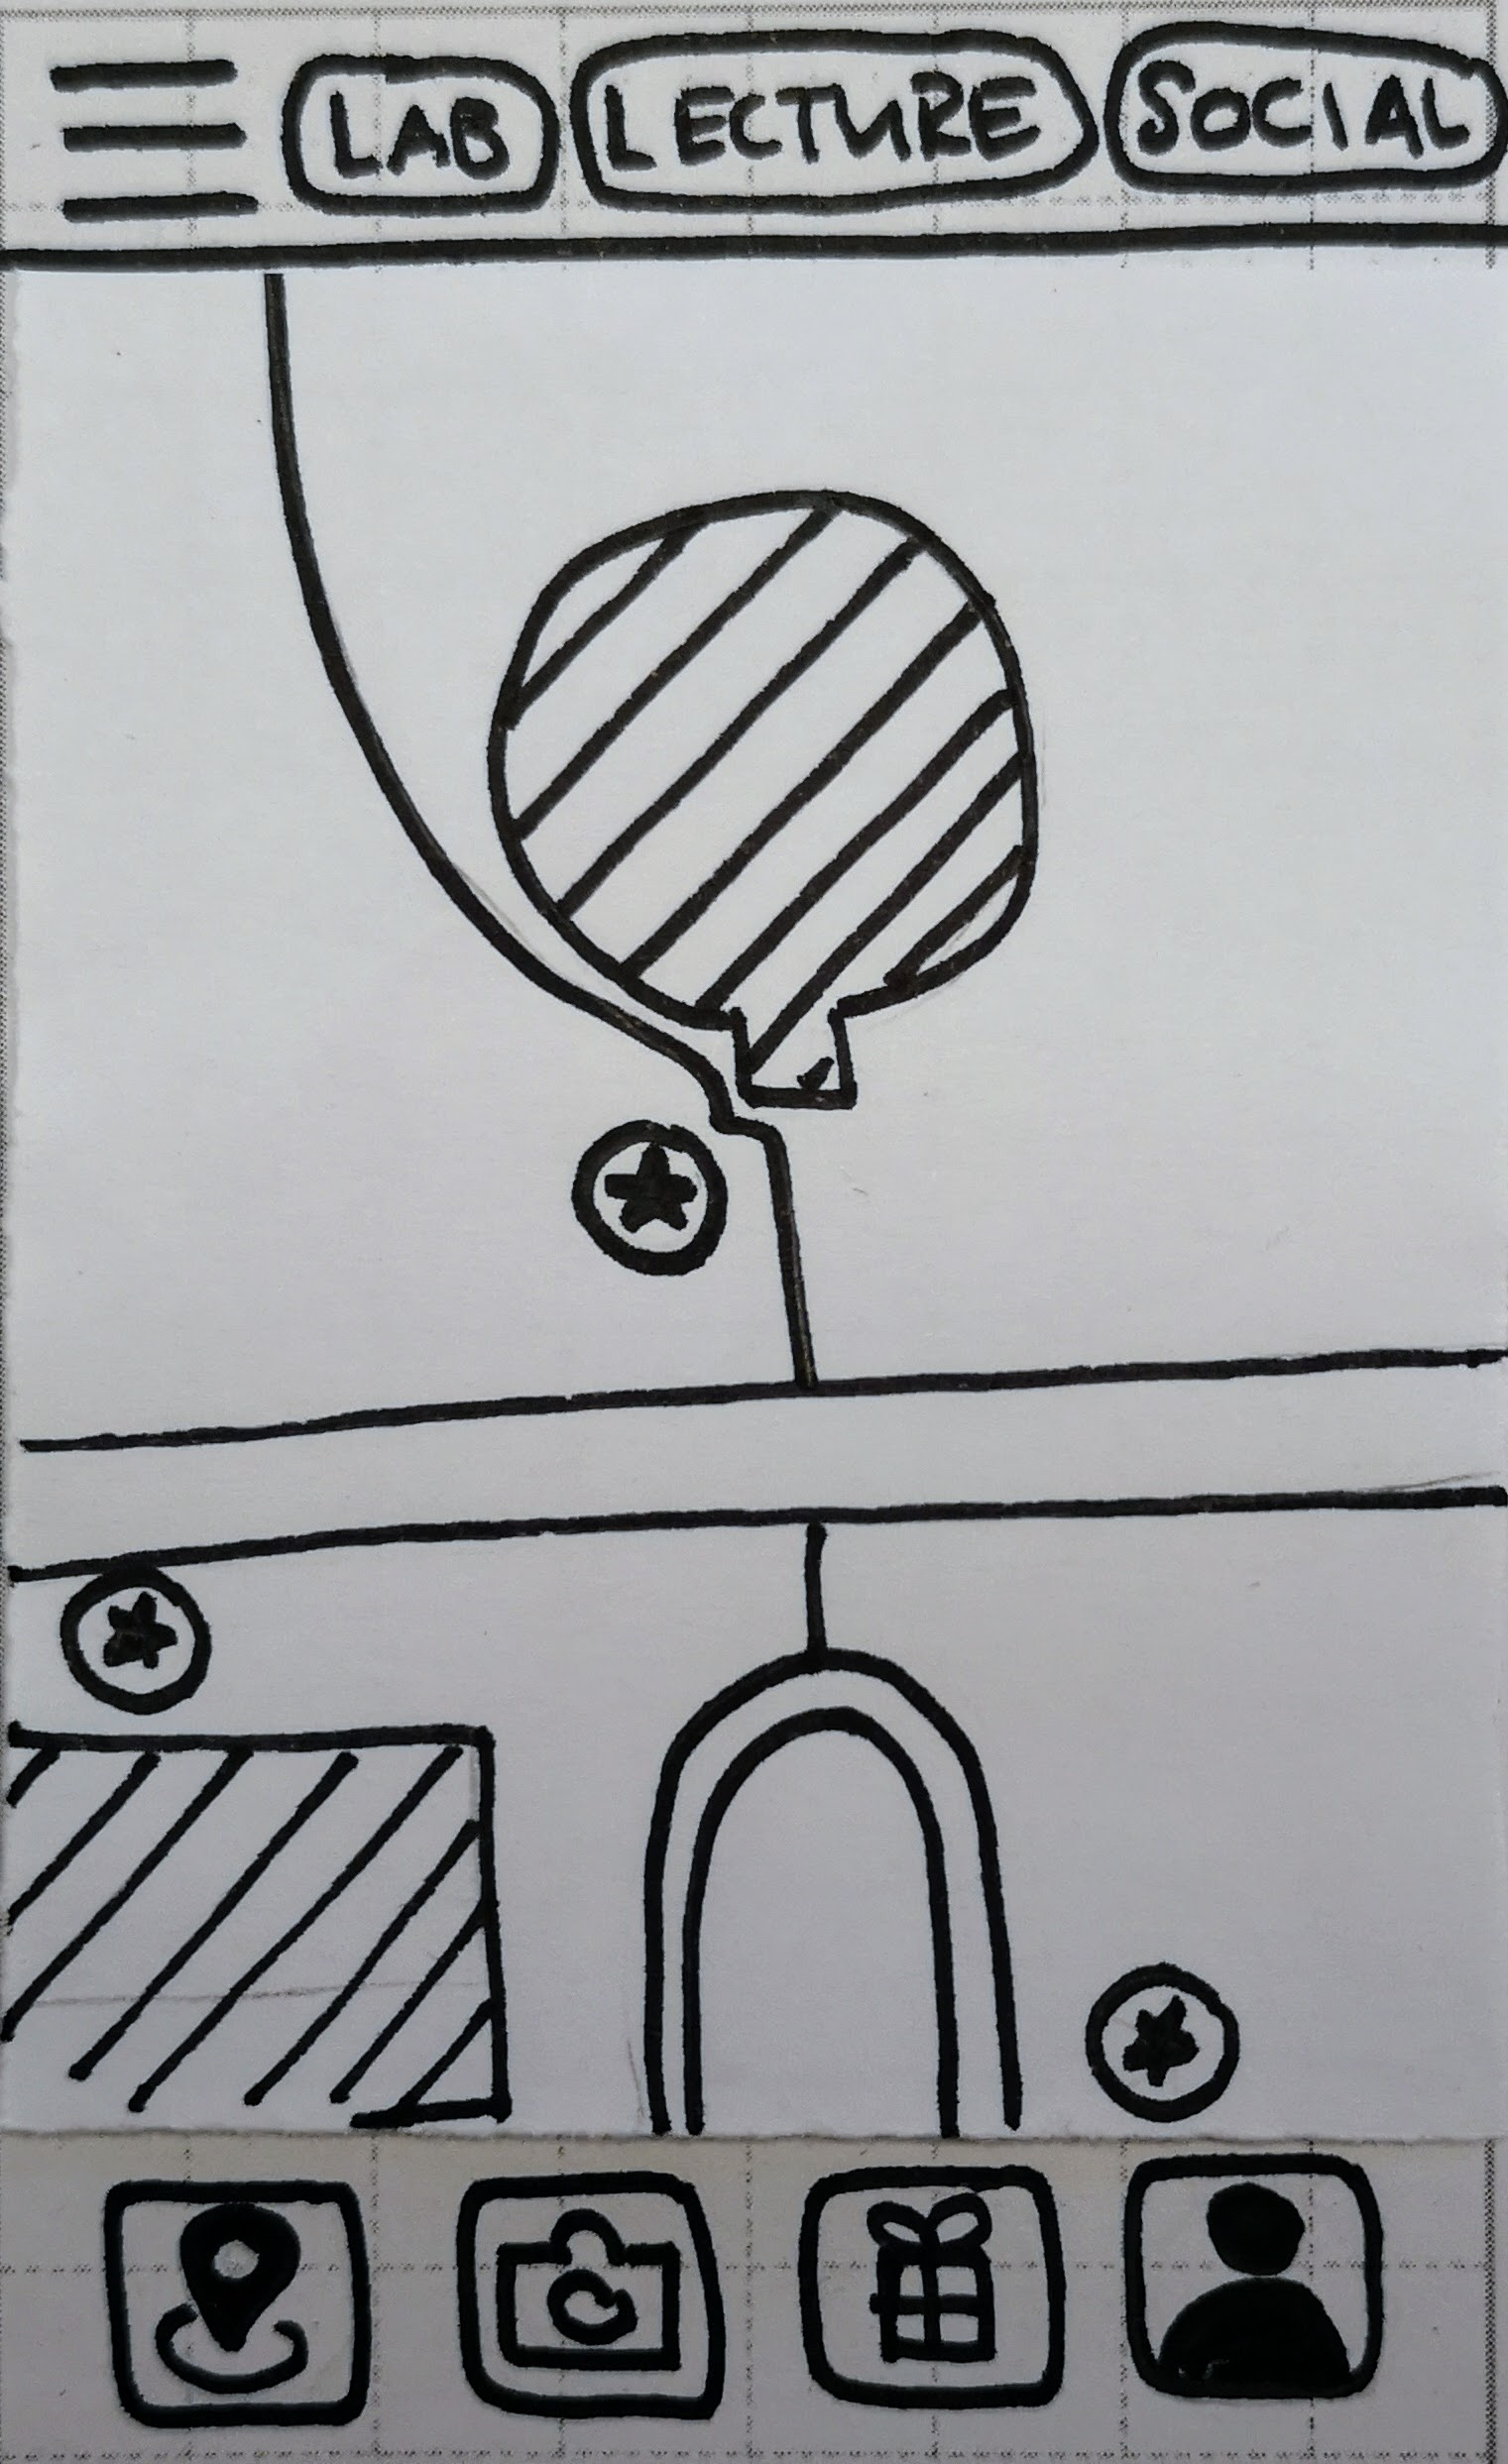
\includegraphics[width=0.3\textwidth]{./figures/refined_proto/2.jpg}

\newpage
\subsection*{Appendix C - Initial Storyboards}
%\documentclass[12pt]{beamer}

\usepackage{pgfpages}
%\usepackage{handoutWithNotes}


\setbeameroption{show notes on second screen=right}

\setbeamertemplate{note page}{\pagecolor{white!5}\insertnote}\usepackage{palatino}

\begin{document}

\begin{frame}
  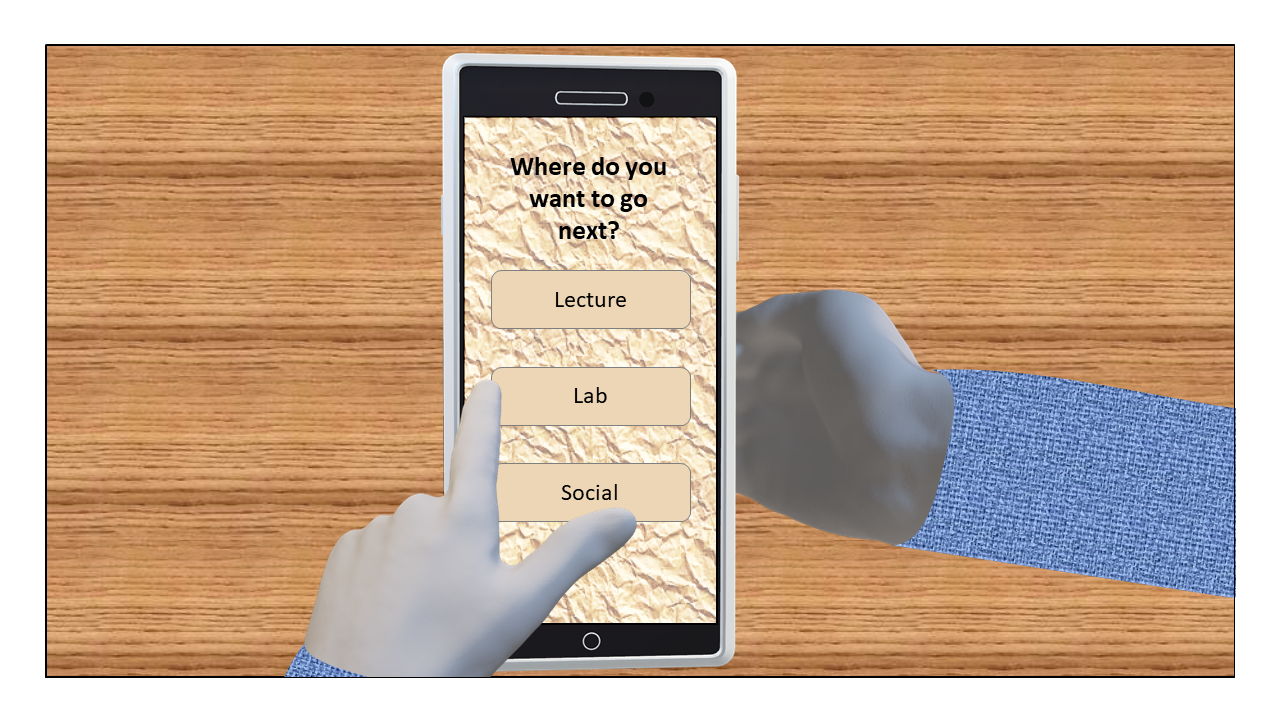
\includegraphics[width=\paperwidth]{./figures/initial_storyboards/Slide2.png}
  \note{
    Alan can choose what kind of location he wants to go next.
    He sees three buttons on the middle of the screen, and he taps one.    
  }
\end{frame}

\begin{frame}
  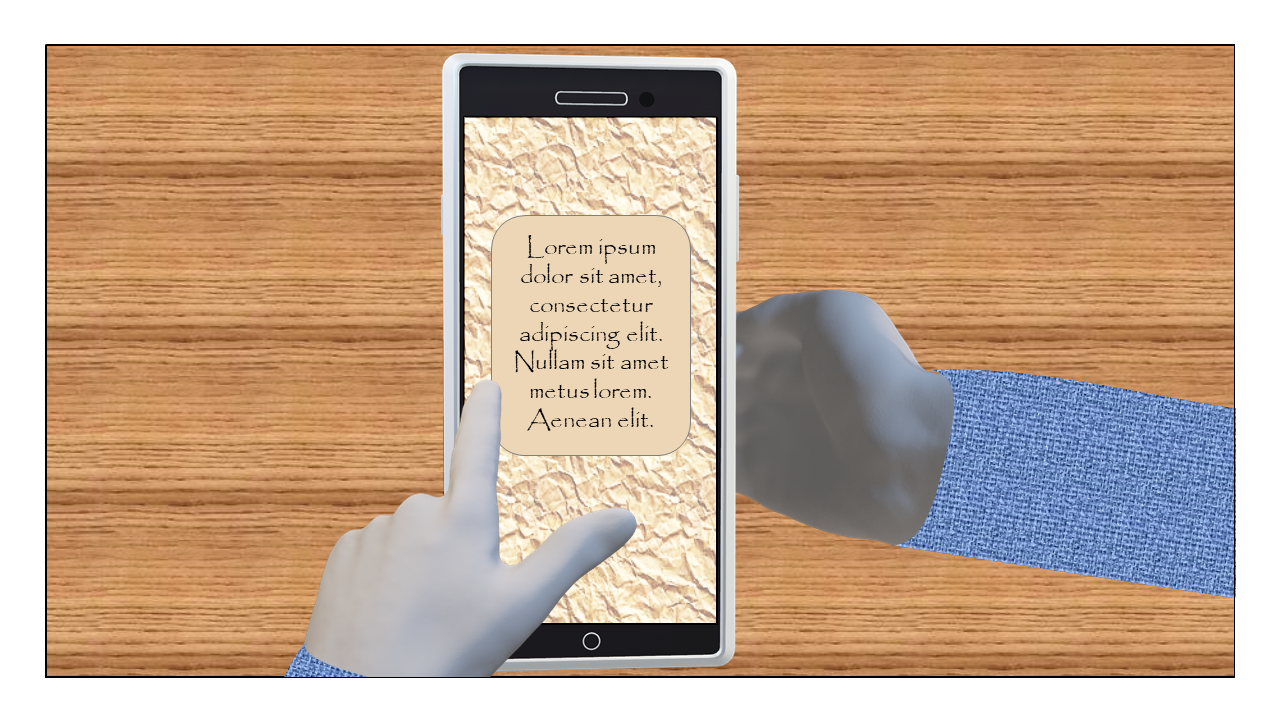
\includegraphics[width=\paperwidth]{./figures/initial_storyboards/Slide3.png}
  \note{
    The screen changes – the buttons are hidden, and are replaced by a singular riddle.
    He takes some time to think about where the riddle may lead him, what location it can describe.
    Once he is confident in his solution, he locks his phone, puts it in his pocket, and heads to the location.    
  }
\end{frame}

\begin{frame}
  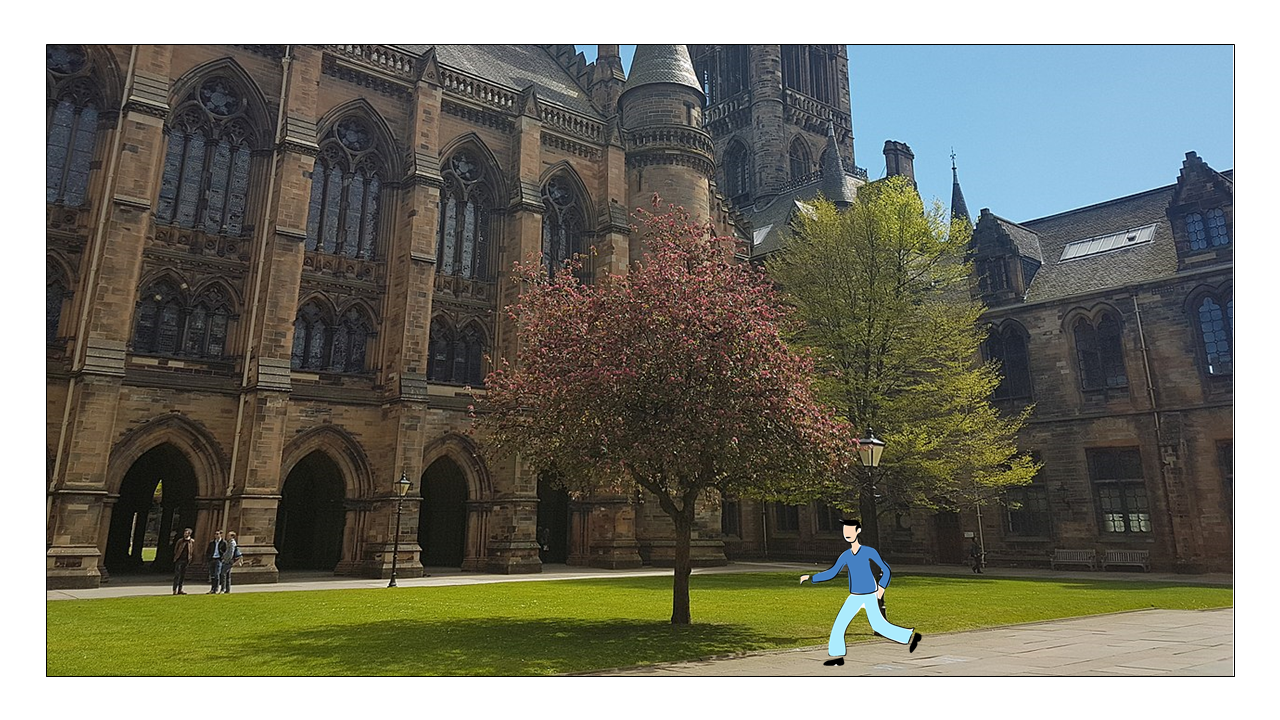
\includegraphics[width=\paperwidth]{./figures/initial_storyboards/Slide4.png}
  \note{
    Alan heads to the building he believes the solution is in.
    He has his phone in his pocket, as he does not need it for navigation.
    The app does not show him where the solution of the riddle is or how to get there.
    When he is uncertain about his solution, he steps to the side to not block anyone’s path, and looks at the riddle again to refresh his memory.    
  }
\end{frame}

\begin{frame}
  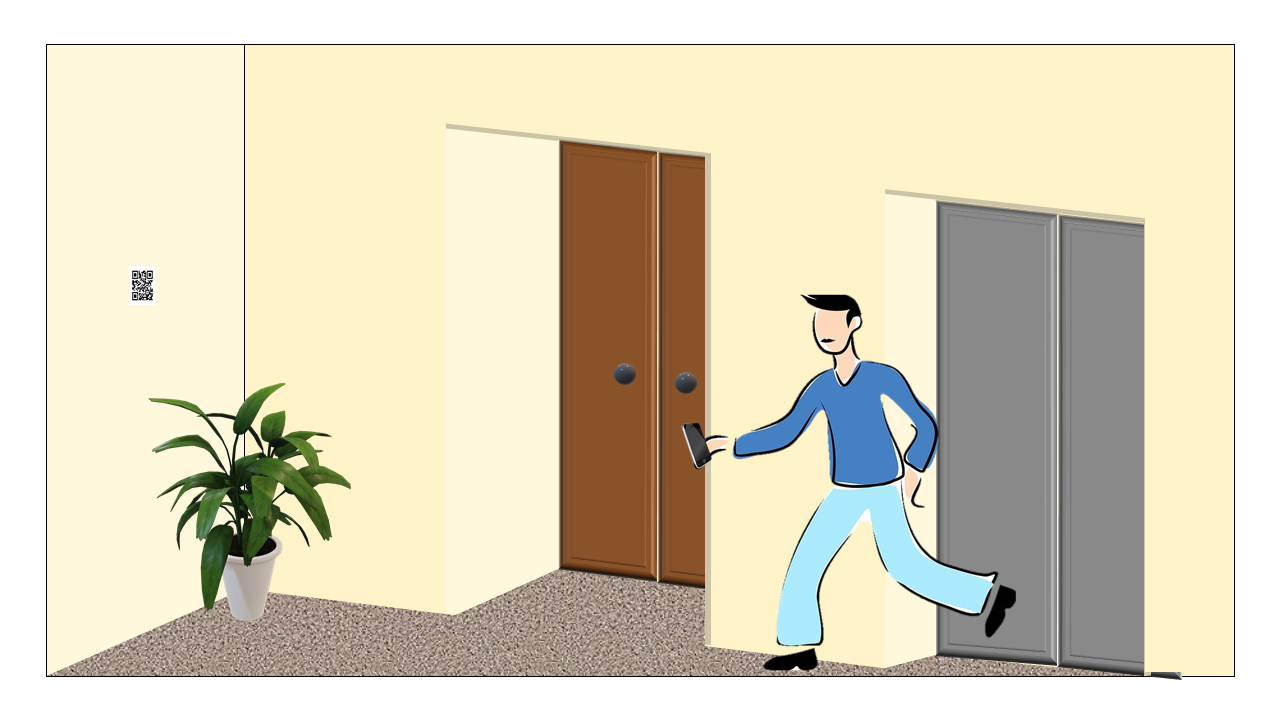
\includegraphics[width=\paperwidth]{./figures/initial_storyboards/Slide5.png}
  \note{
    Alan steps out of the elevator and notices the QR code.
    He is happy that his intuition was correct, and he solved the riddle correctly.
    He proceeds to the code, not blocking other people’s entrance to the lab.
    He takes out his phone from his pocket to open the app and check in at the checkpoint.    
  }
\end{frame}

\begin{frame}
  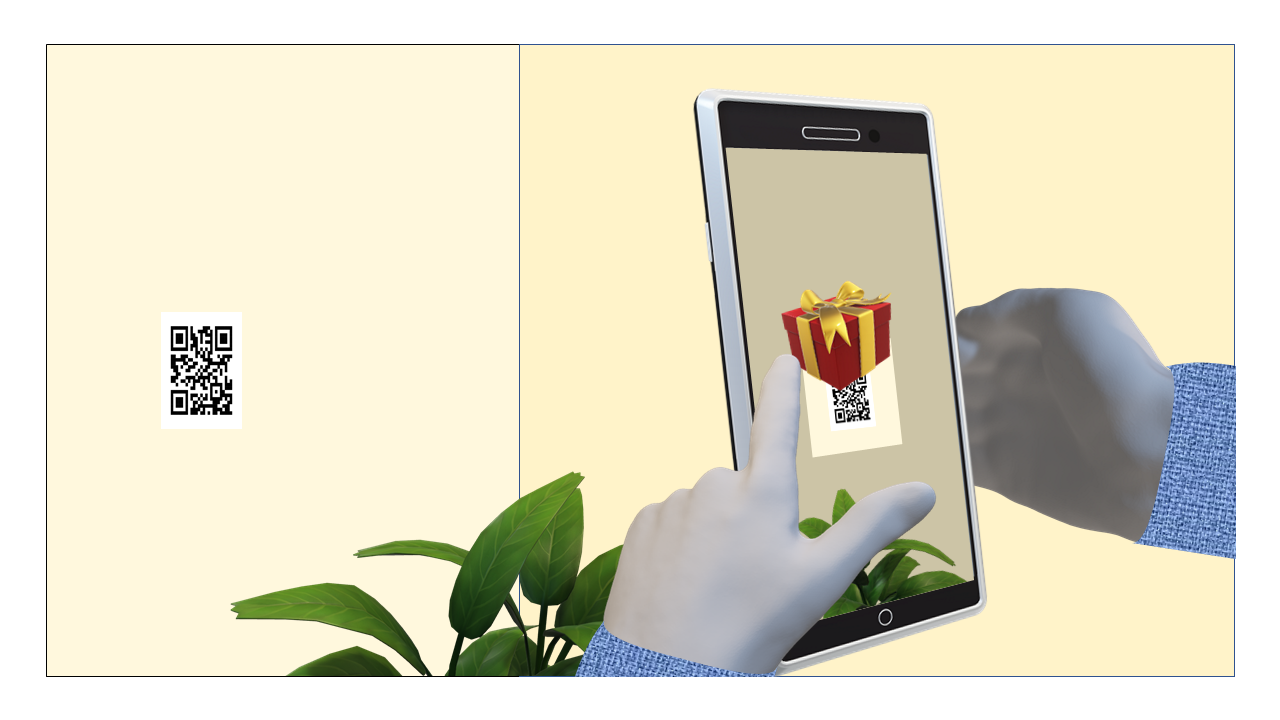
\includegraphics[width=\paperwidth]{./figures/initial_storyboards/Slide6.png}
  \note{
    Alan taps on the camera button at bottom of the screen.
    The screen quickly changes as the build in camera feature opens in the app.
    The screen shows a bounding box with grey tint on the screen outside the bounding box – this shows Alan that he needs to move the QR code inside the bounding box to scan it.
    The AR representation of a checkpoint item then appears on the screen on top of the QR code, and moves in space with the phone as long as the QR code stays within bounding box.    
  }
\end{frame}

\begin{frame}
  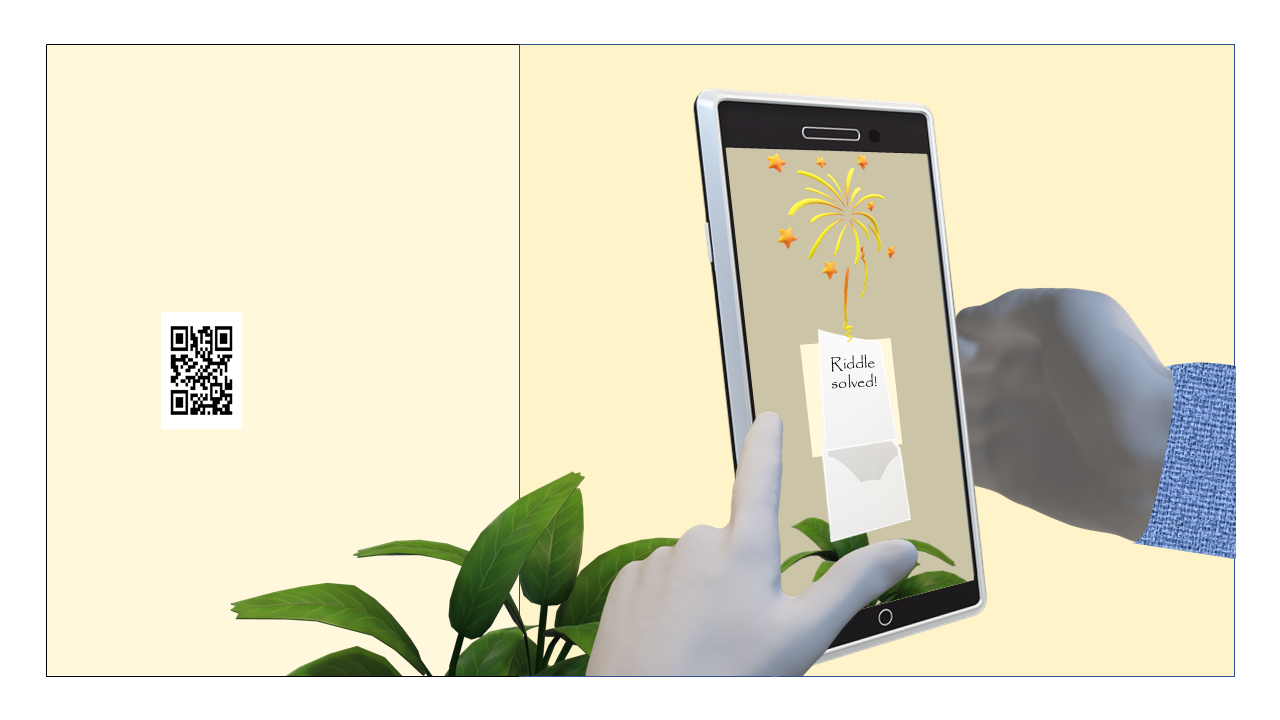
\includegraphics[width=\paperwidth]{./figures/initial_storyboards/Slide7.png}
  \note{
    Alan taps on the checkpoint item he is presented with.
    If the riddle was solved correctly and Alan arrived at the location the riddle told him to, the phone vibrates three times to signal to him he succeeded. At the same time, a small, triumphant sound effect plays to collaborate the physical feedback.
    The screen also changes, and a small animation of an envelope opening happens.
    From the envelope fireworks appear and a popup tells Alan he scanned the location and the riddle was solved.
    The app then tells him all the XP he’s gained, if he has levelled up, and if he gained any new freebies.    
  }
\end{frame}

\begin{frame}
  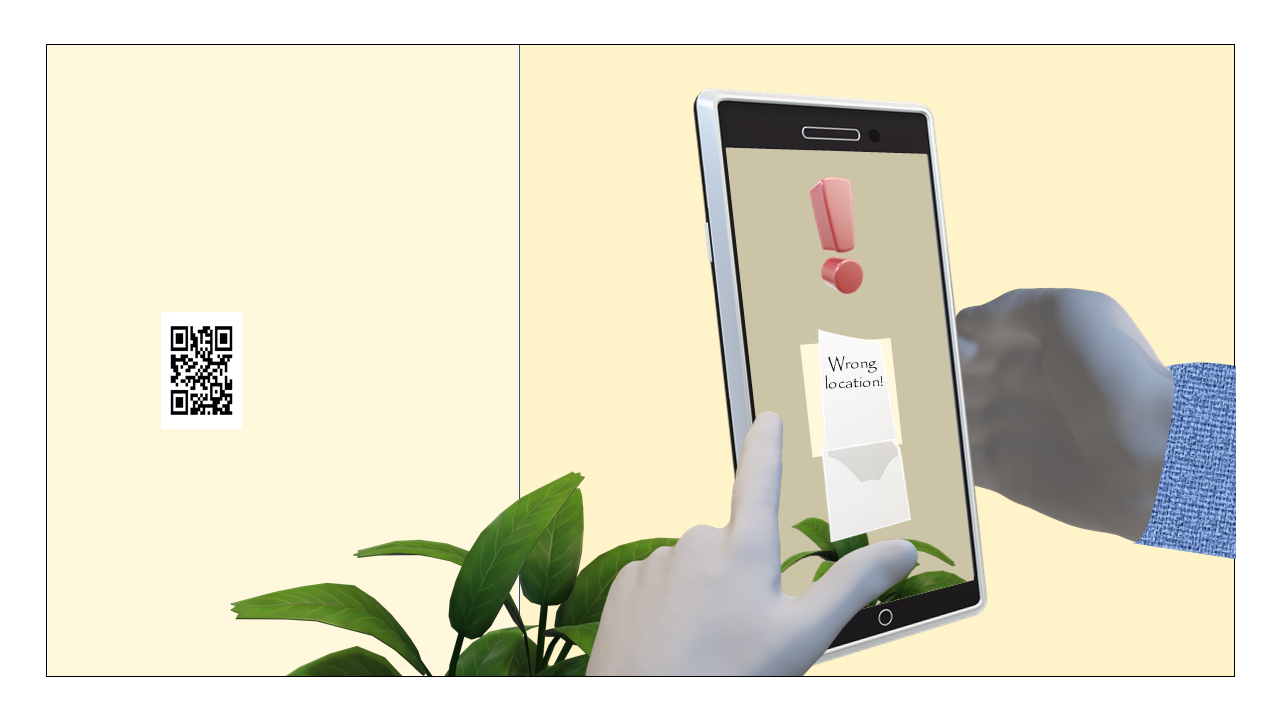
\includegraphics[width=\paperwidth]{./figures/initial_storyboards/Slide8.png}
  \note{
    Alan taps on the checkpoint item he is presented with.
    If the riddle was solved incorrectly and Alan arrived at a location different to what the riddle told him to, the phone vibrates twice to signal to him he got the answer wrong.
    The screen also changes, and a small animation of an envelope opening happens.
    From the envelope a red exclamation point appears and a popup tells Alan that he is in the wrong location.
    The application then presents him with the option to register this location as the wrong answer to the riddle, or to not register the check-in and allow him to try figure out the correct answer.    
  }
\end{frame}

\begin{frame}
    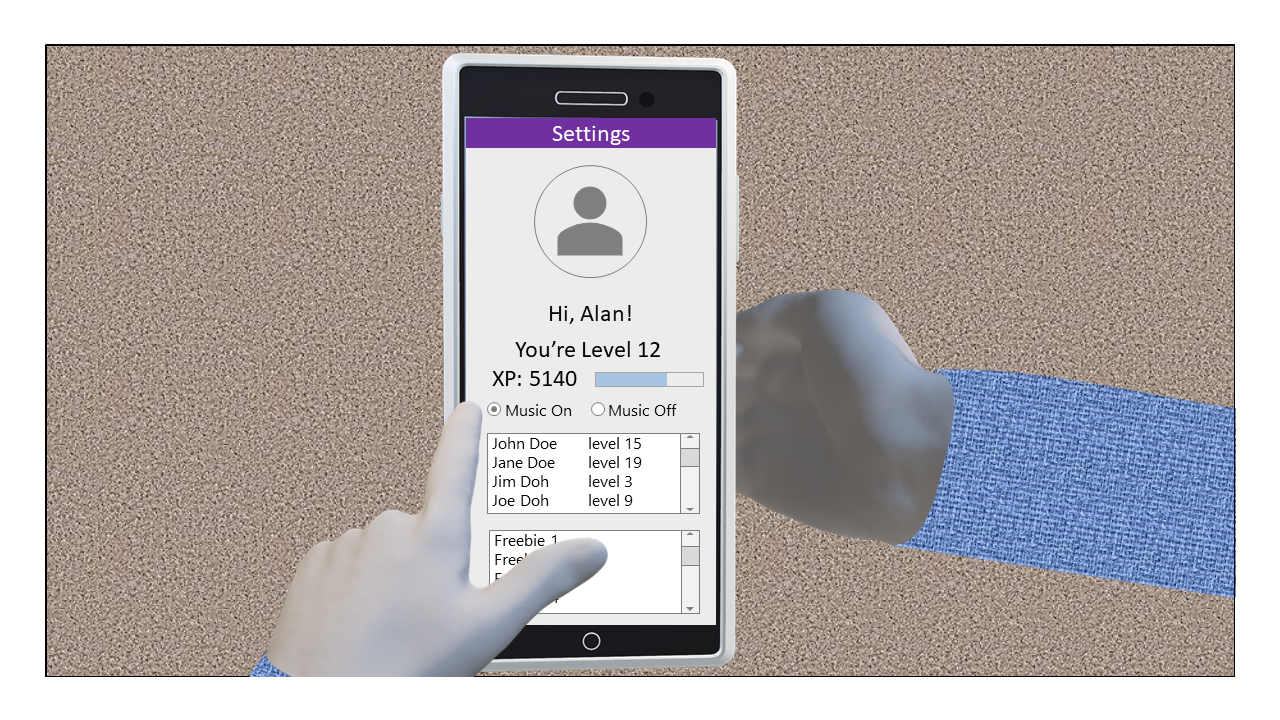
\includegraphics[width=\paperwidth]{./figures/initial_storyboards/Slide9.png}
    \note{
        After having completed a checkpoint, Alan views his in-game progress.
He does so by tapping on the Settings button at the main screen. 
He views his XP, his list of friends, his in-game level, his badges earned, and can also adjust the app settings or log out if he wants to.
He is pleased to see he is close to levelling up, and with the new level, he is to gain new freebies.
    }
  \end{frame}
  
\end{document}
\begin{center}
  \noindent\makebox[\textwidth]{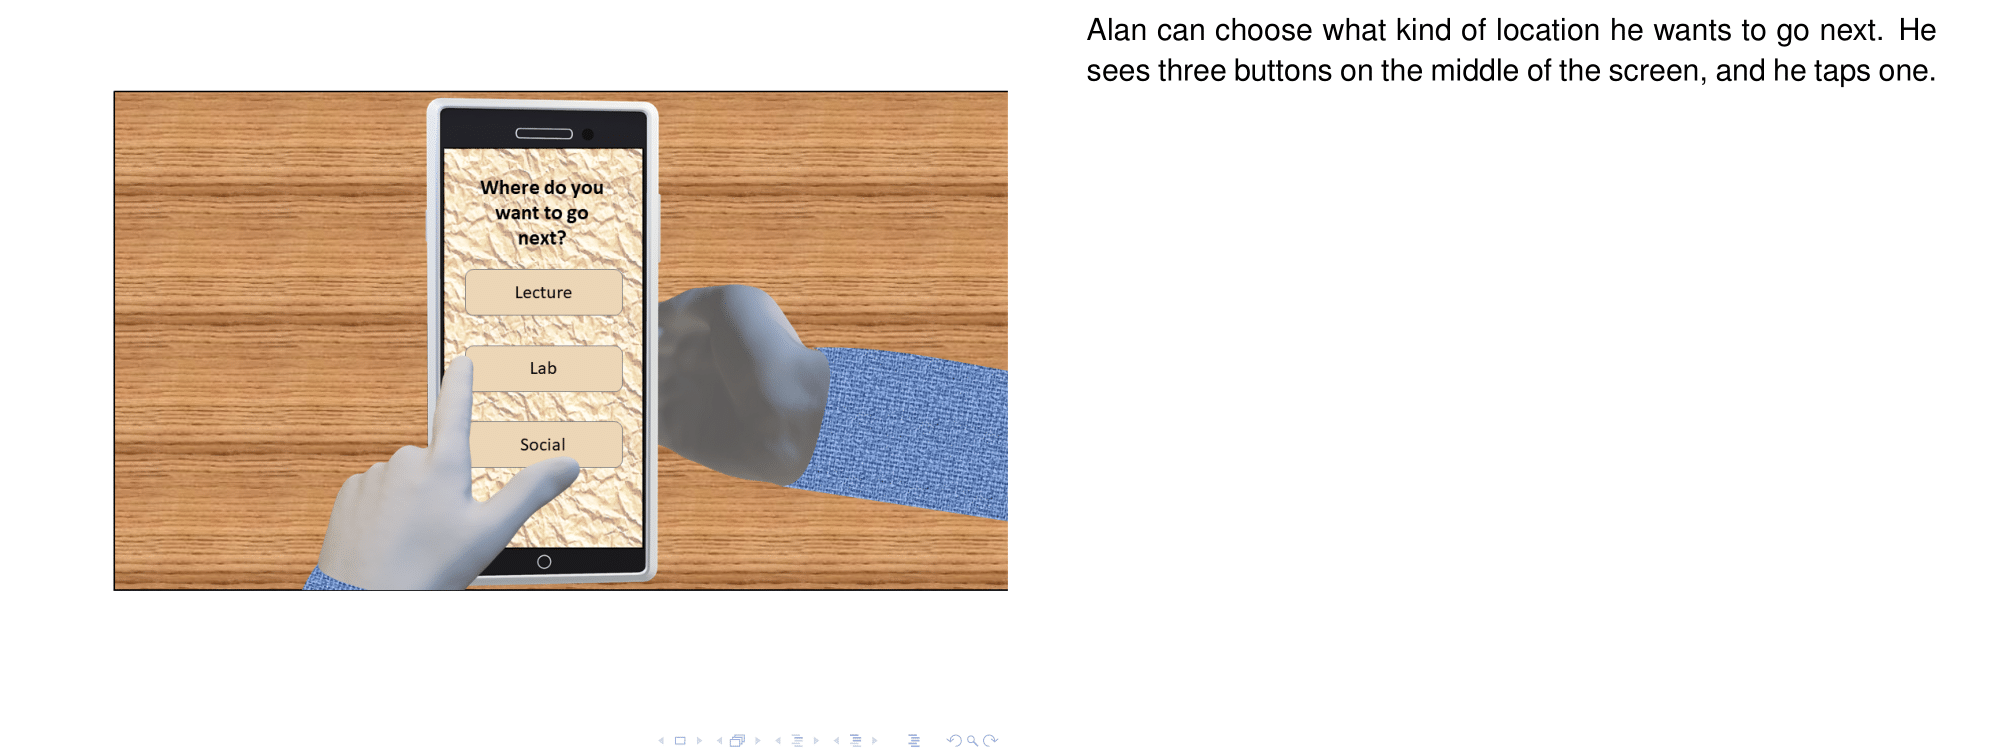
\includegraphics[width=\paperwidth]{./figures/initialStoryboards/initialStoryboards-1.png}}
\end{center}
\begin{center}
  \noindent\makebox[\textwidth]{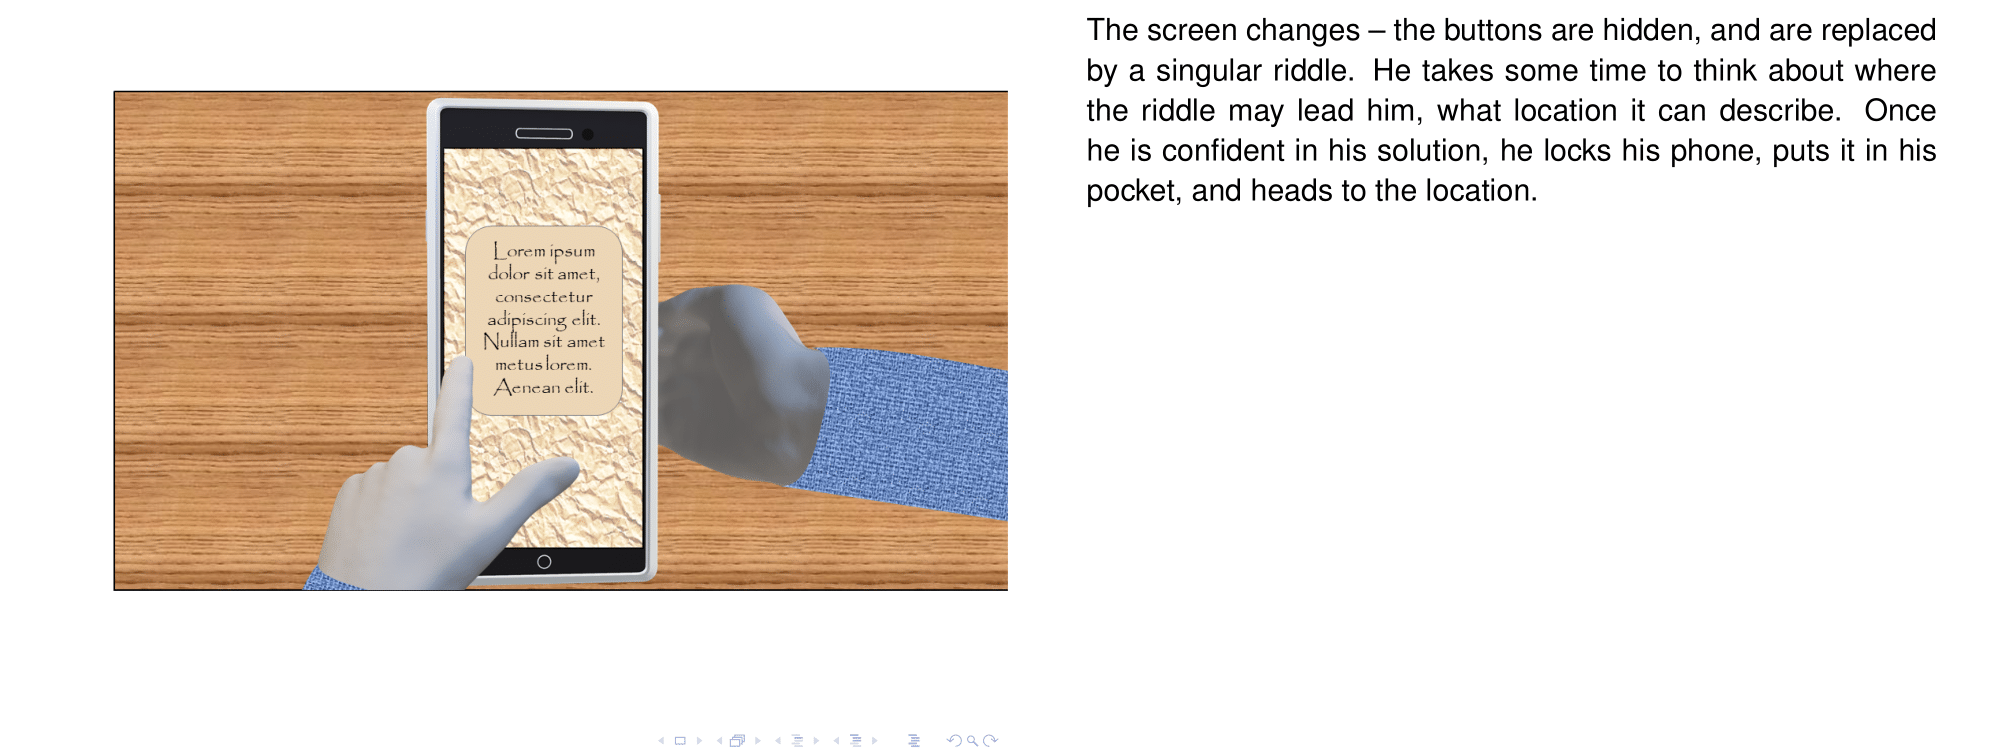
\includegraphics[width=\paperwidth]{./figures/initialStoryboards/initialStoryboards-2.png}}
\end{center}
\begin{center}
  \noindent\makebox[\textwidth]{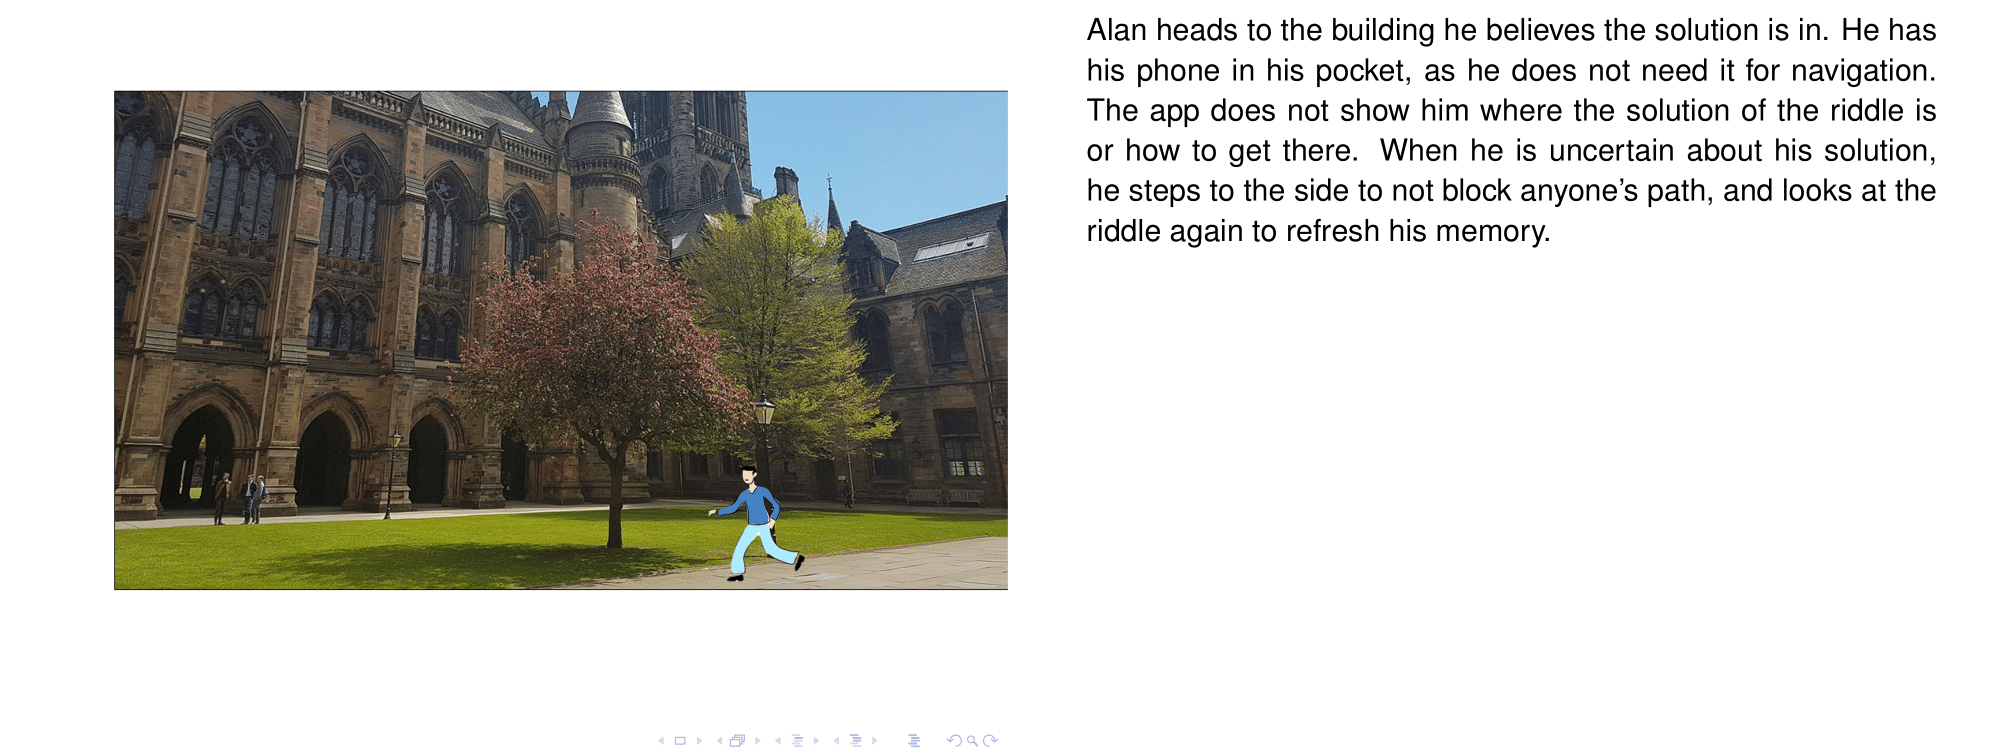
\includegraphics[width=\paperwidth]{./figures/initialStoryboards/initialStoryboards-3.png}}
\end{center}
\begin{center}
  \noindent\makebox[\textwidth]{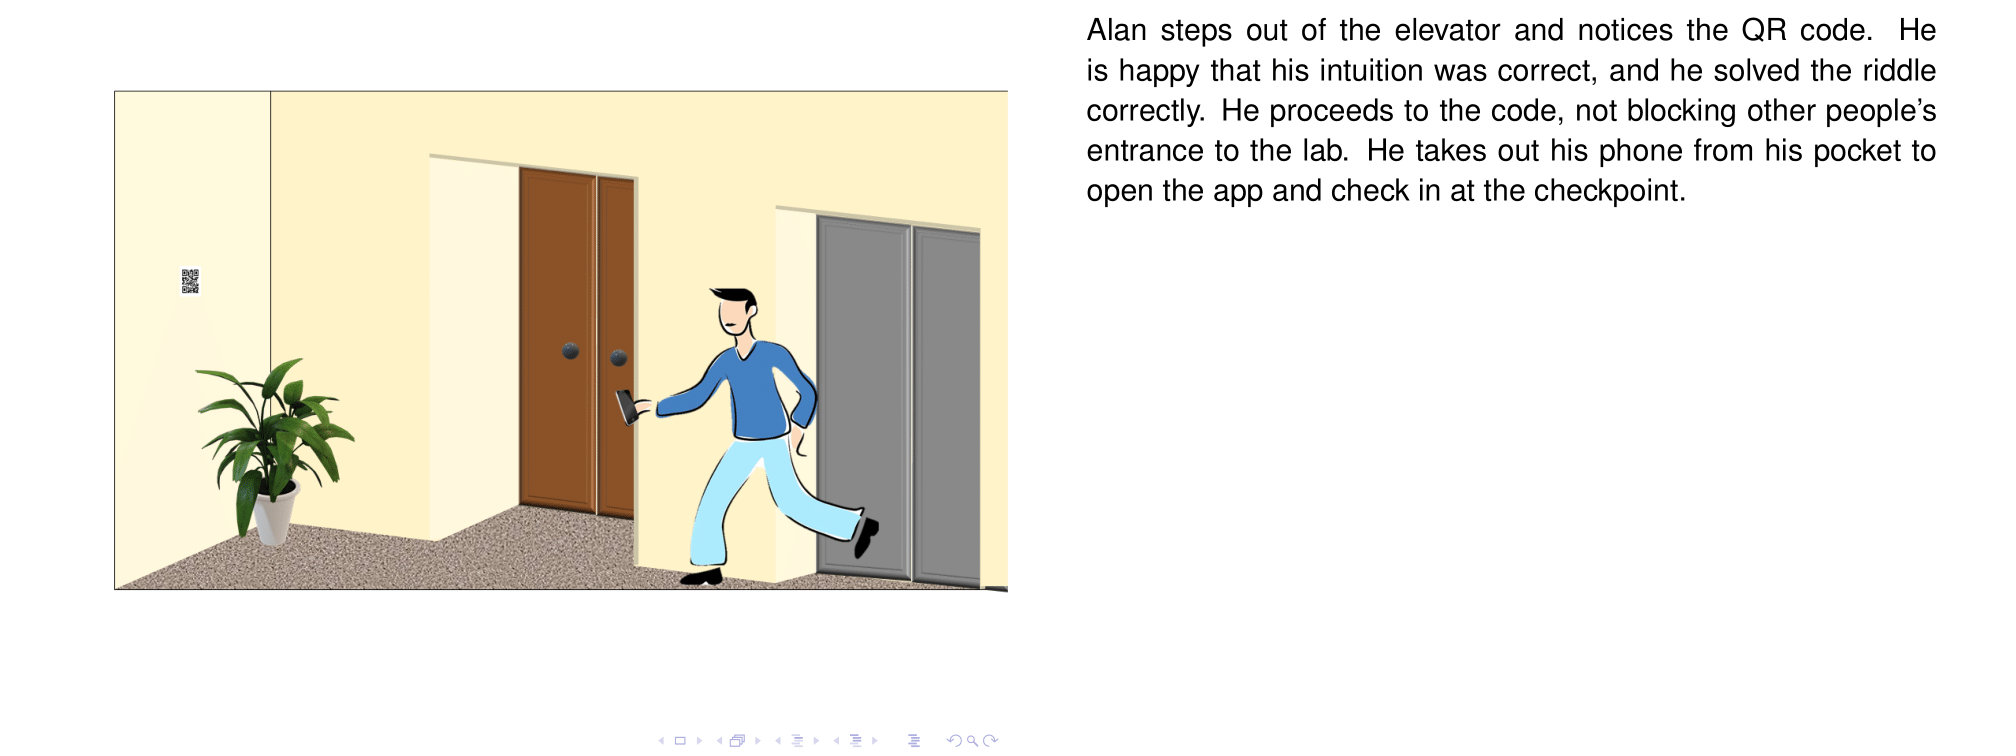
\includegraphics[width=\paperwidth]{./figures/initialStoryboards/initialStoryboards-4.png}}
\end{center}
\begin{center}
  \noindent\makebox[\textwidth]{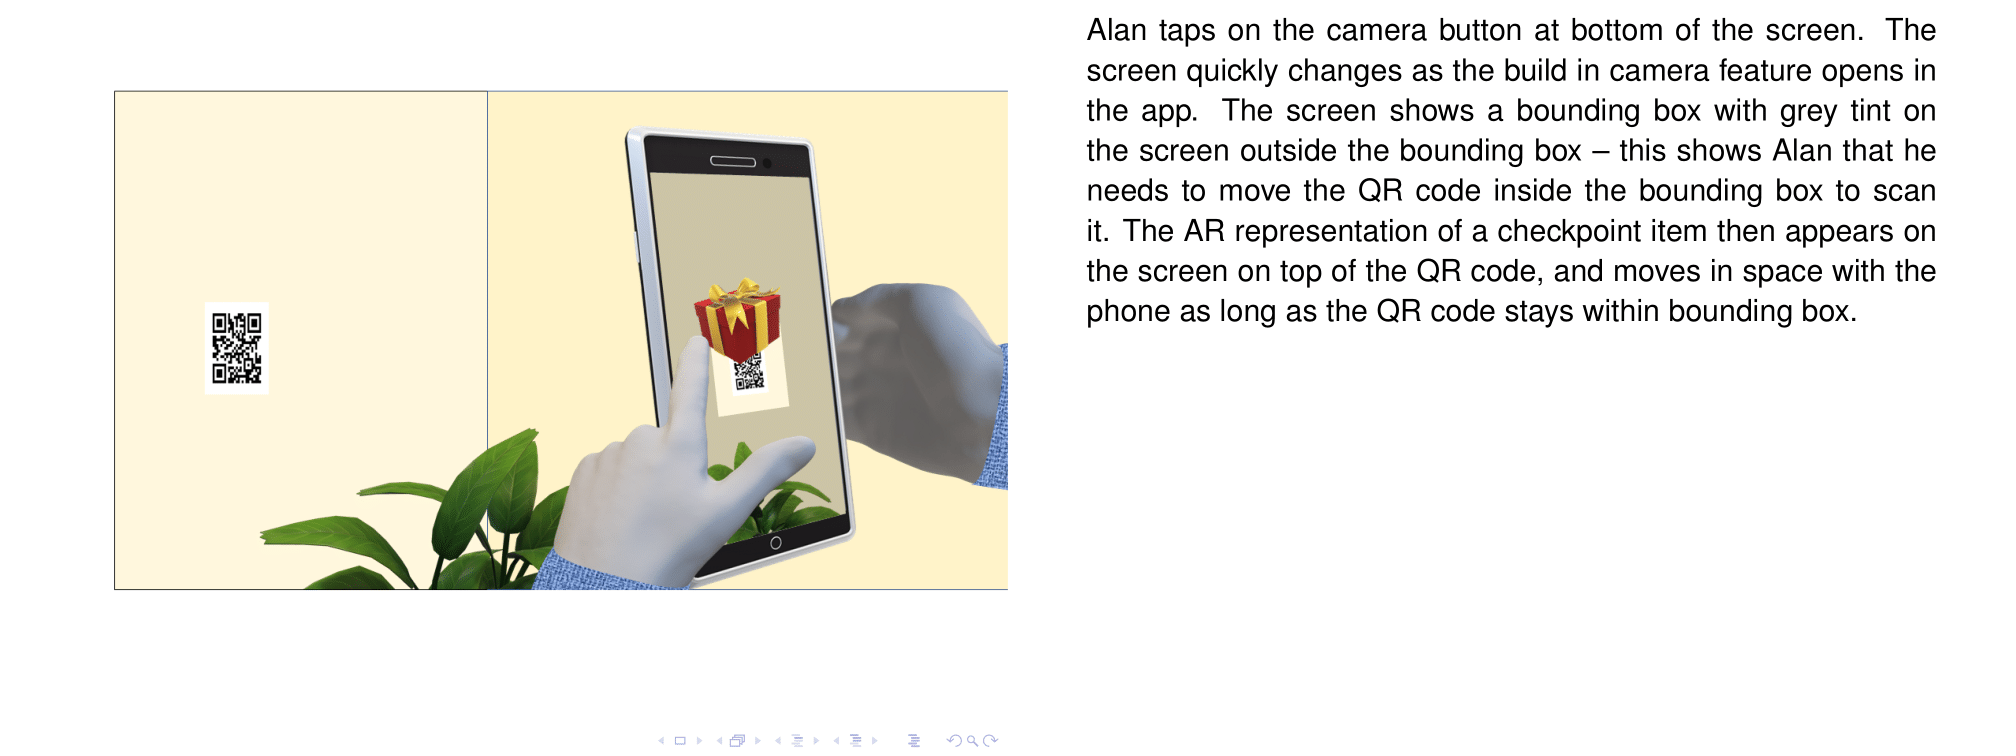
\includegraphics[width=\paperwidth]{./figures/initialStoryboards/initialStoryboards-5.png}}
\end{center}
\begin{center}
  \noindent\makebox[\textwidth]{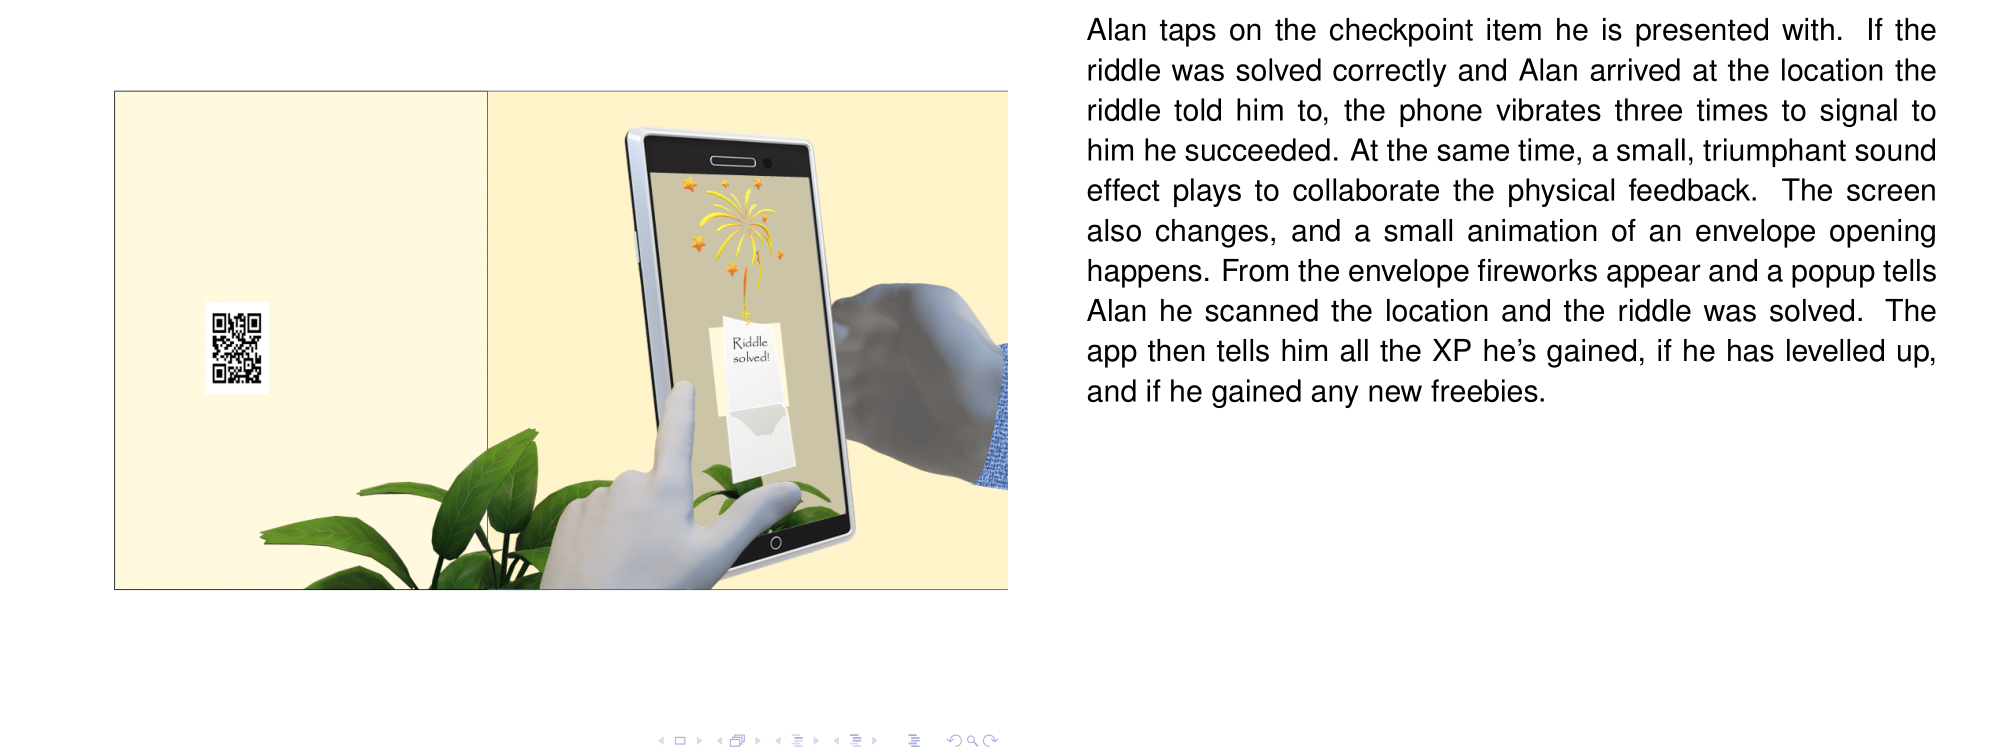
\includegraphics[width=\paperwidth]{./figures/initialStoryboards/initialStoryboards-6.png}}
\end{center}
\begin{center}
  \noindent\makebox[\textwidth]{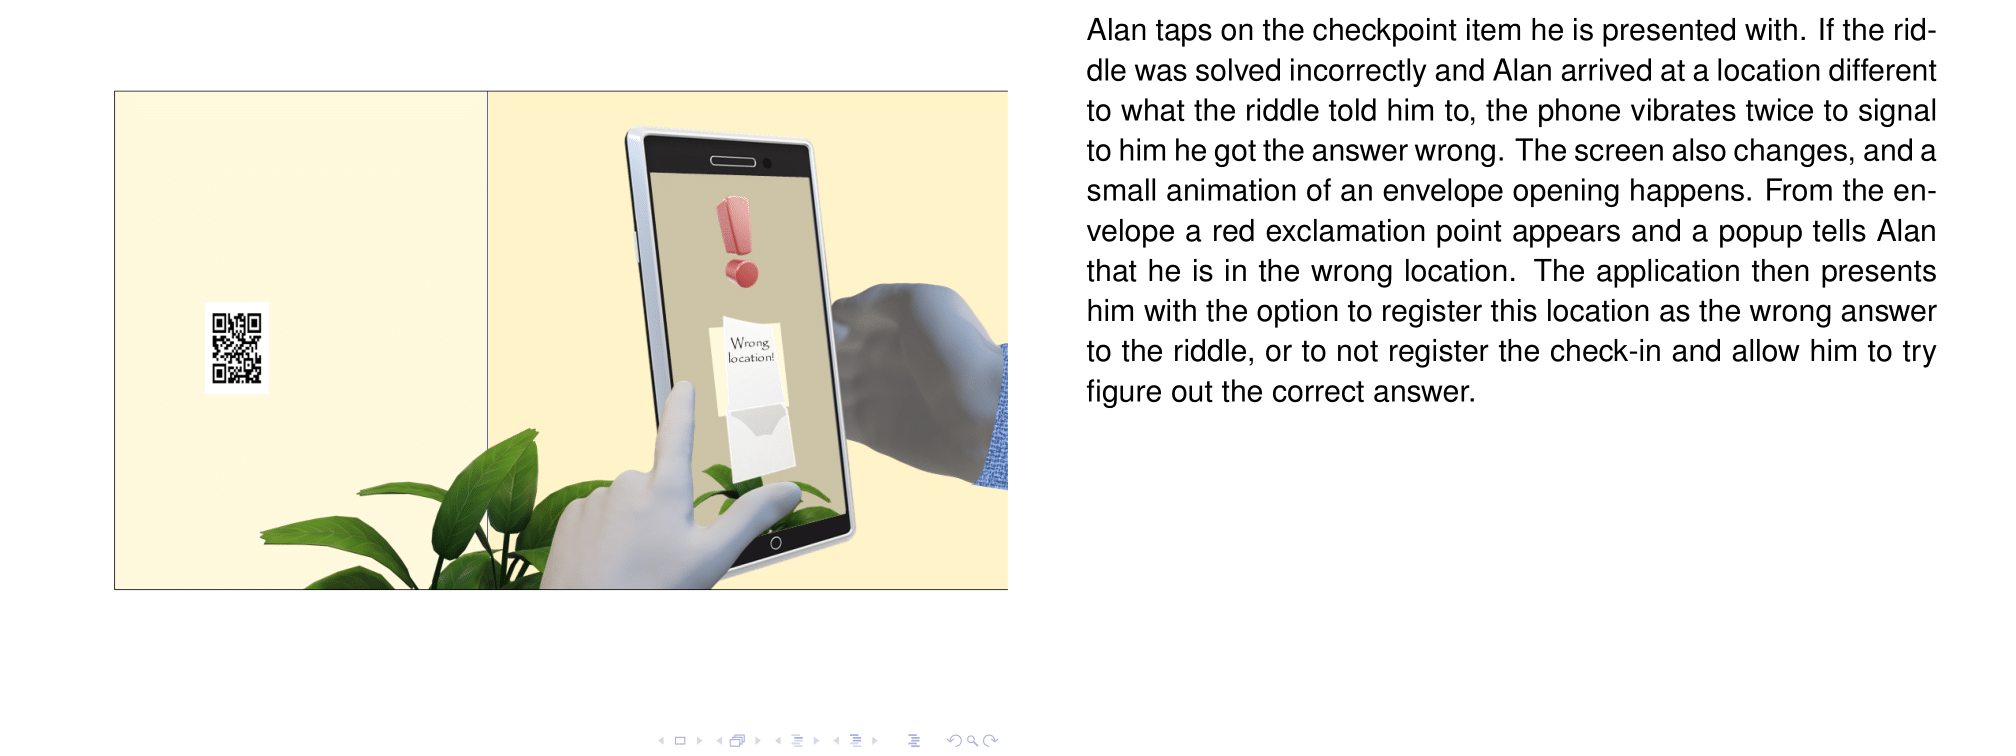
\includegraphics[width=\paperwidth]{./figures/initialStoryboards/initialStoryboards-7.png}}
\end{center}
\begin{center}
  \noindent\makebox[\textwidth]{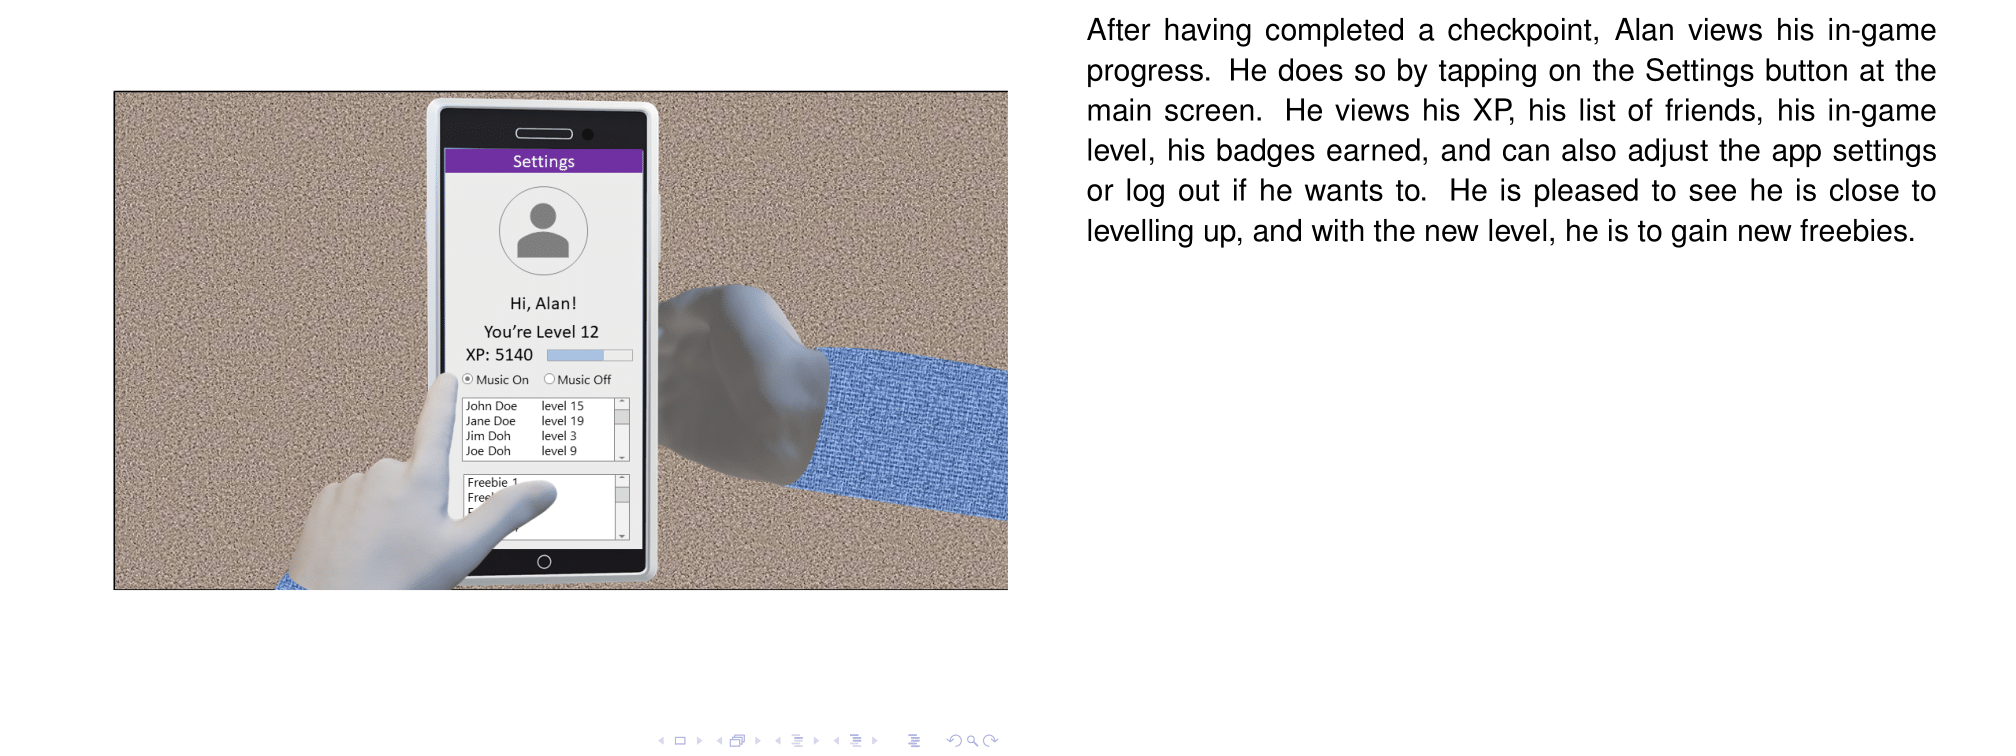
\includegraphics[width=\paperwidth]{./figures/initialStoryboards/initialStoryboards-8.png}}
\end{center}

\newpage
\subsection*{Appendix D - Final Storyboards}
%\documentclass[12pt]{beamer}

\usepackage{pgfpages}
%\usepackage{handoutWithNotes}


\setbeameroption{show notes on second screen=right}

\setbeamertemplate{note page}{\pagecolor{white!5}\insertnote}\usepackage{palatino}

\begin{document}

\begin{frame}
  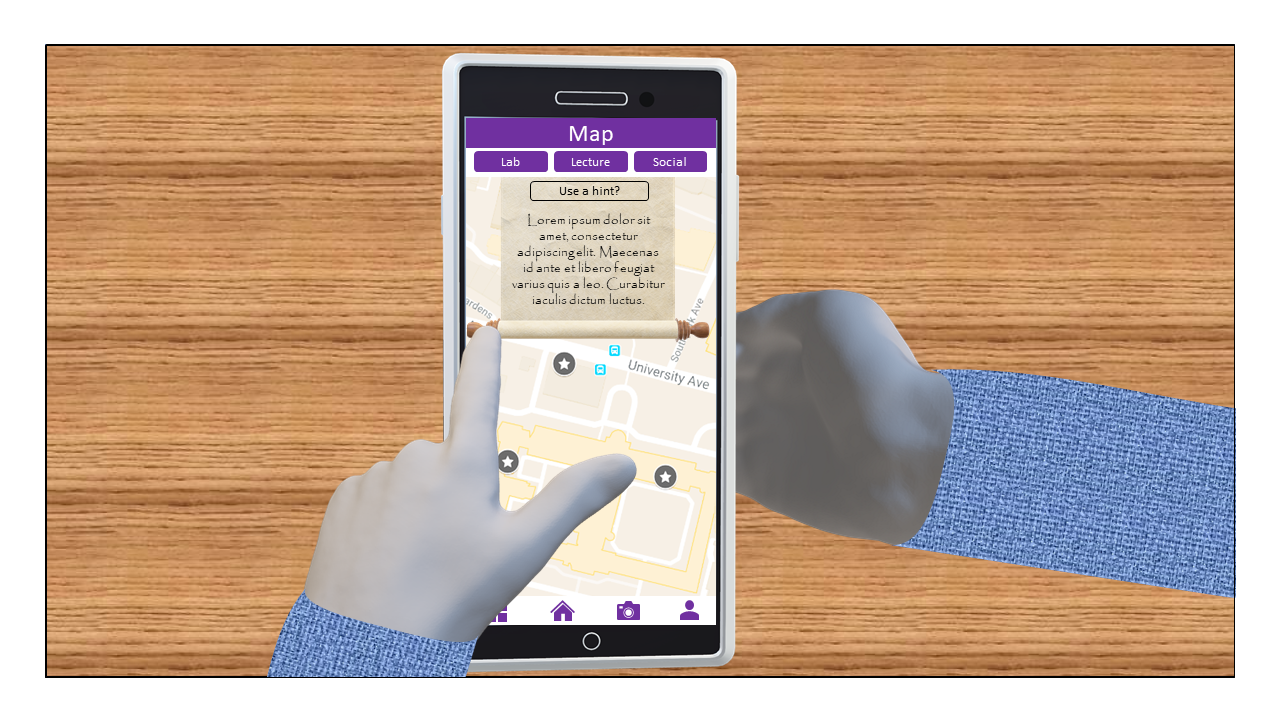
\includegraphics[width=\paperwidth]{./figures/final_storyboards/Slide11.png}
  \note{After completing the personality test, Alan chooses to view the map to discover where there are locations, and to be able to choose his first riddle.
  By tapping the button for one of the three types of location at the top of the screen overlapping the map, he starts that riddle.
  The riddle “unravels” like an ancient roll, and rolls down from the top of the screen to halfway through it, leaving space for Alan to read the riddle clearly and still see the map underneath.
  As the riddle is unravelling, the phone plays a subtle sound effect, similar to that of old paper scroll rolling.
  Once he is done reading the riddle, he swipes up or taps on the riddle and it hides itself by rolling up and disappearing behind the buttons.
  As the riddle is rolling up, the phone plays the scroll sound effect again.
  }
\end{frame}

\begin{frame}
  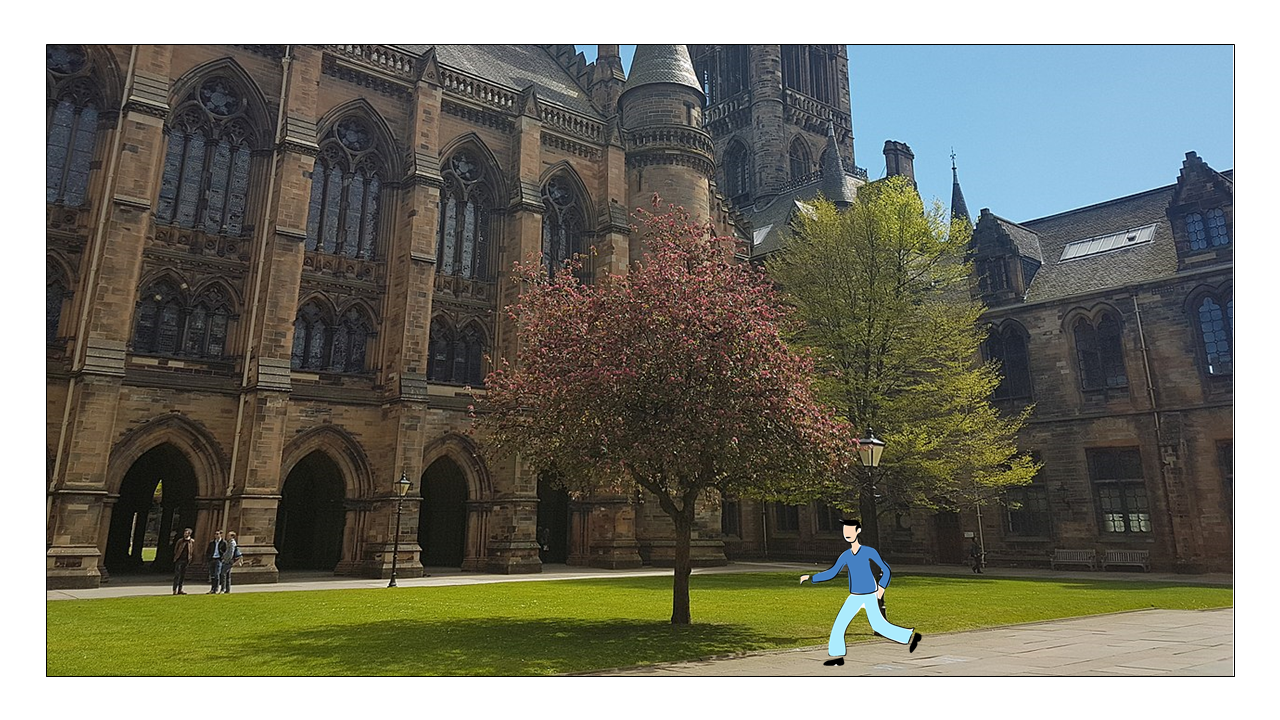
\includegraphics[width=\paperwidth]{./figures/final_storyboards/Slide12.png}
  \note{Alan heads to the building he believes the solution is in.
  He has his phone in his pocket, as he does not need it for navigation.
  He has a choice to take it out to look at the map and find locations, but the app does not show him where the solution of the riddle is or how to get there.
  }
\end{frame}

\begin{frame}
  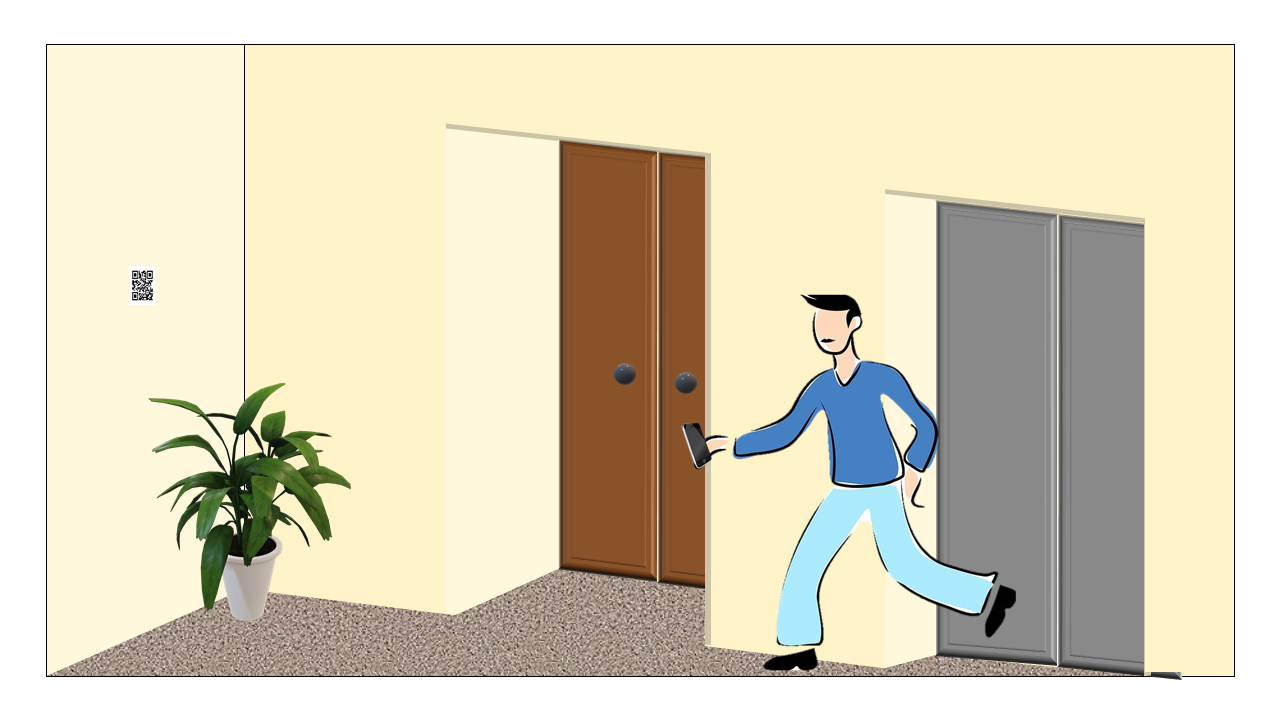
\includegraphics[width=\paperwidth]{./figures/final_storyboards/Slide13.png}
  \note{Alan steps out of the elevator and notices the QR code.
  He is happy that his intuition was correct, and he solved the riddle correctly.
  He proceeds to the code, not blocking other people’s entrance to the lab.
  He takes out his phone from his pocket to open the app and check in at the checkpoint.
  }
\end{frame}

\begin{frame}
  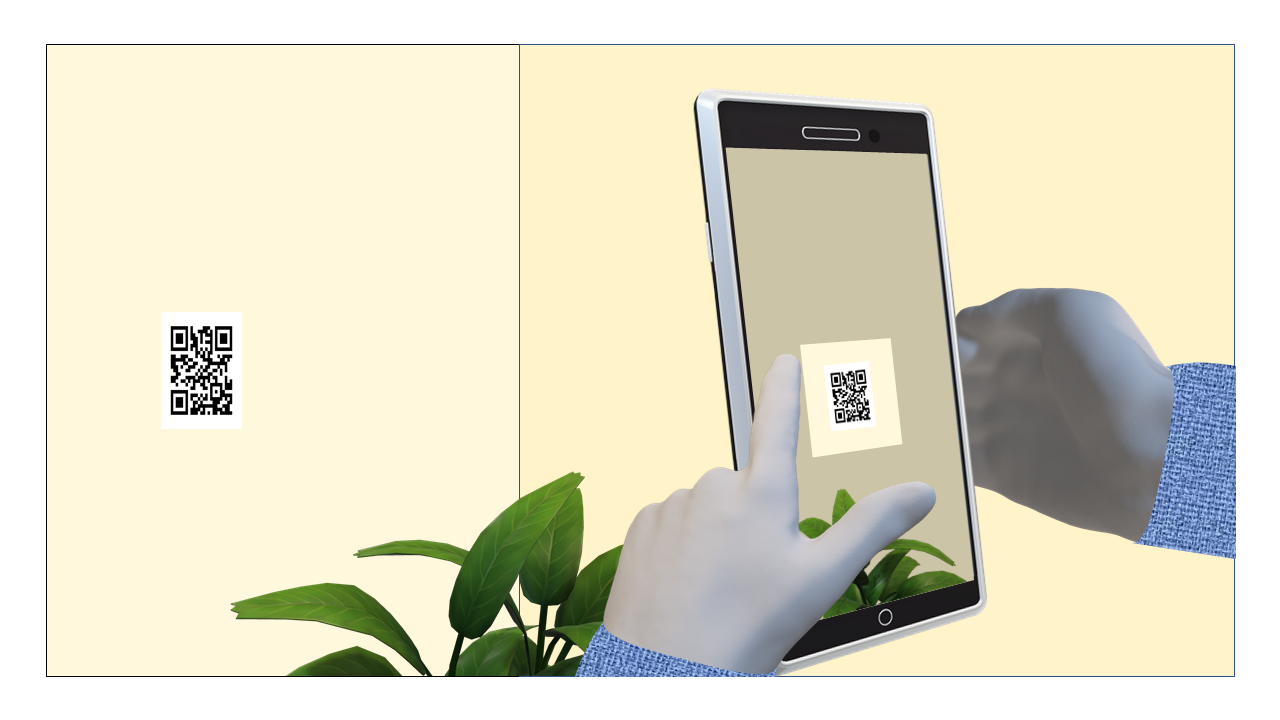
\includegraphics[width=\paperwidth]{./figures/final_storyboards/Slide14.png}
  \note{Alan taps on the camera button at bottom of the screen.
  The phone gives him audio feedback by playing a subtle “pop” sound, similar to that of mobile Operating Systems allocating for keyboard taps.
  The screen quickly changes as the build in camera feature opens in the app.
  The screen shows a bounding box with grey tint on the screen outside the bounding box – this shows Alan that he needs to move the QR code inside the bounding box to scan it.
  When the app registers the code, the phone slightly vibrates once to show Alan it was successfully read.
  }
\end{frame}

\begin{frame}
  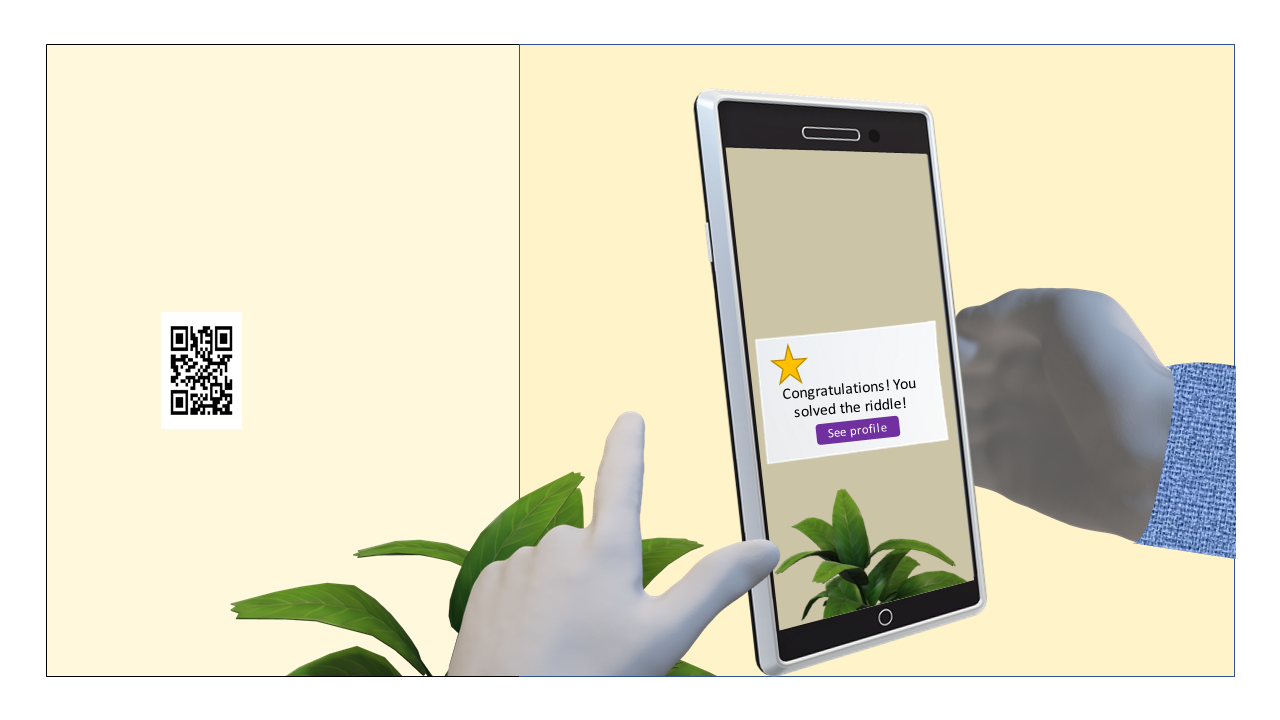
\includegraphics[width=\paperwidth]{./figures/final_storyboards/Slide15.png}
  \note{If the riddle was solved correctly and Alan arrived at the location the riddle told him to, the phone vibrates three times to signal to him he succeeded. At the same time, a small, triumphant sound effect plays to collaborate the physical feedback.
The screen also changes, and a popup tells Alan he scanned the location and the riddle was solved.
The app then presents him with the option to check his profile and view all the XP he’s gained, if he has levelled up, and if he gained any new freebies.
  }
\end{frame}

\begin{frame}
  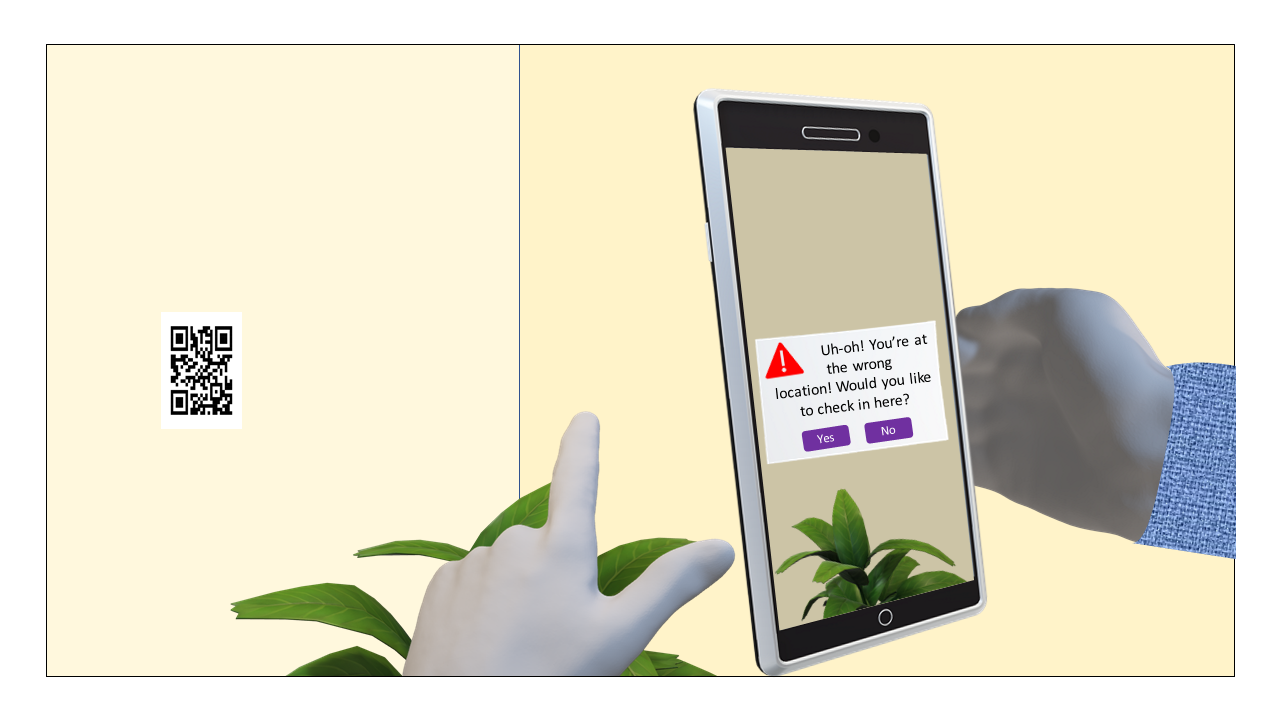
\includegraphics[width=\paperwidth]{./figures/final_storyboards/Slide16.png}
  \note{If the riddle was solved incorrectly and Alan arrived at a location different to what the riddle told him to, the phone vibrates twice to signal to him he got the answer wrong.
The screen also changes, and a popup tells Alan that he is in the wrong location.
The application then presents him with the option to register this location as the wrong answer to the riddle, or to not register the check-in and allow him to try figure out the correct answer.
  }
\end{frame}

\begin{frame}
  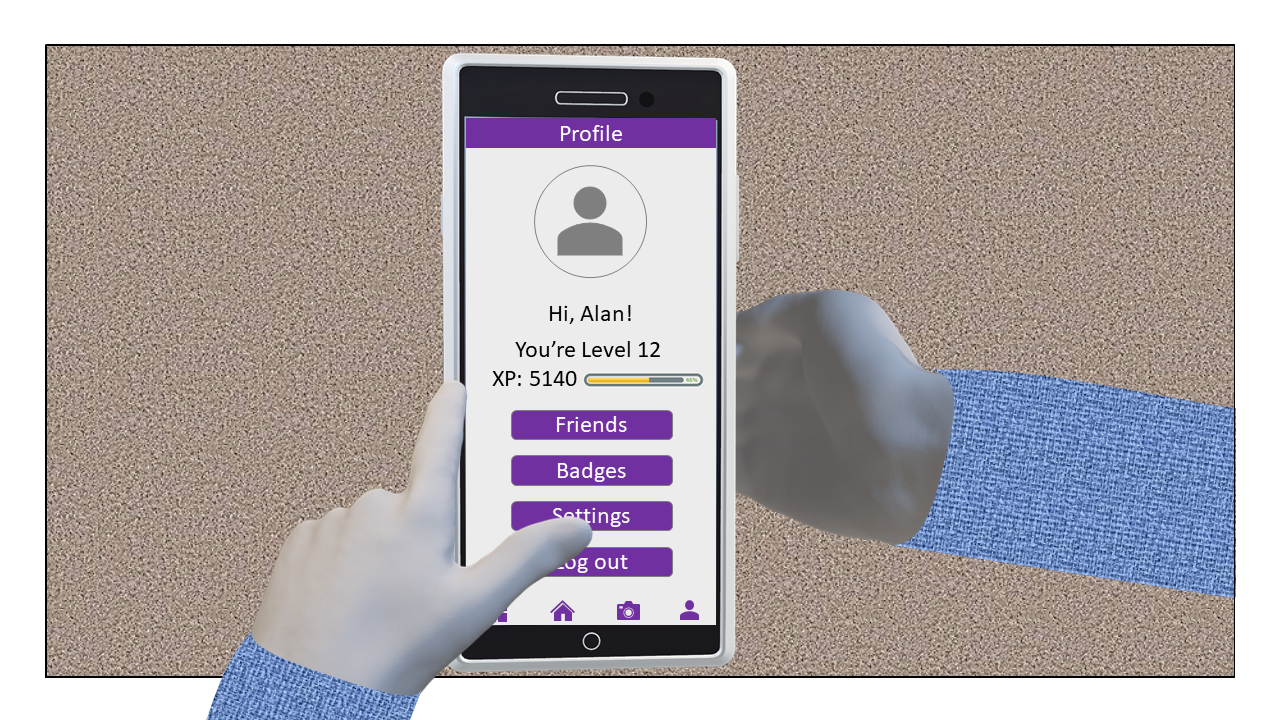
\includegraphics[width=\paperwidth]{./figures/final_storyboards/Slide17.png}
  \note{After having completed a checkpoint, Alan views his in-game progress.
  He does so by tapping on the Profile button at the bottom of the screen.
  With any button press in this screen, the app plays the same “pop” sound effect as on the map menu.
  He views his XP, his list of friends, his in-game level, his badges earned, and can also adjust the app settings or log out if he wants to.
  He is pleased to see he is close to levelling up, and with the new level, he is to gain new freebies.
  }
\end{frame}

\begin{frame}
  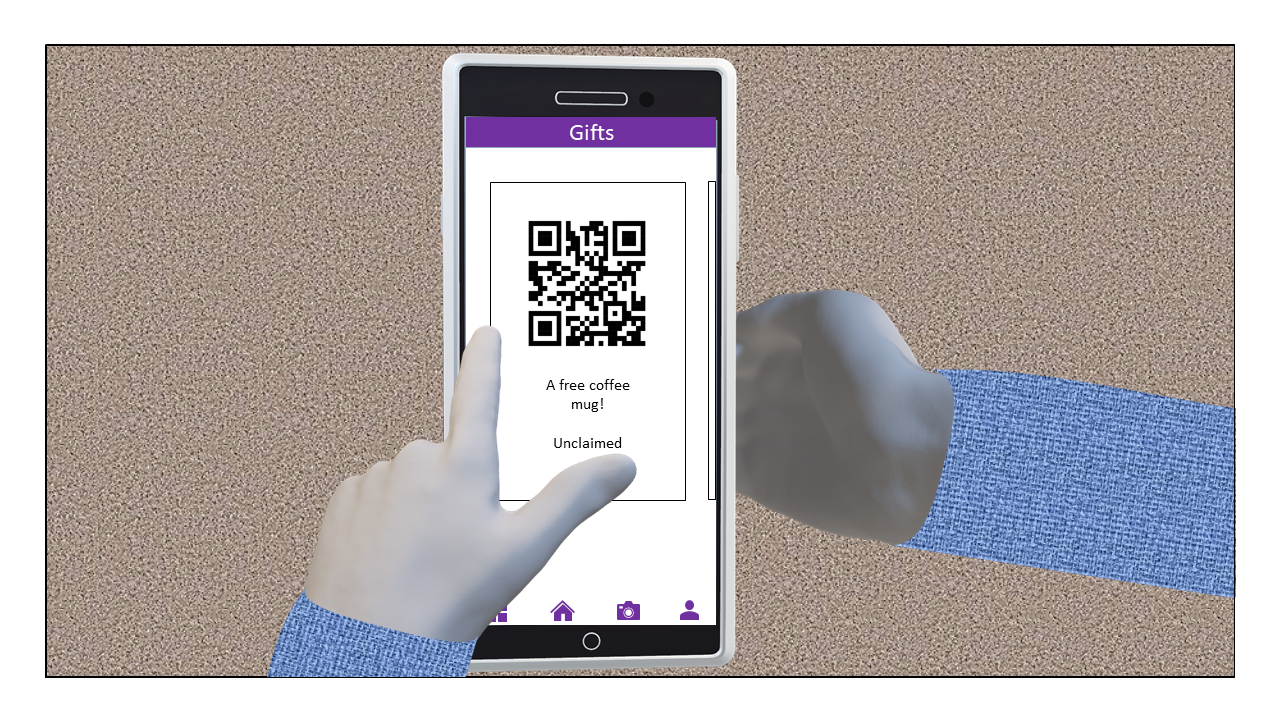
\includegraphics[width=\paperwidth]{./figures/final_storyboards/Slide18.png}
  \note{After having realised that he has gained enough points to qualify for one of the freebies, he views them.
  He does so by tapping on the “Freebies” button at the bottom of the screen.
  When he opens the screen, freebies are contained in smaller item tags, with the next item slightly showing at the right side of the screen.
  This is to signal that Alan can swipe right to see the other freebies.
  When he wants to claim the freebie, he can tap on the freebie item, which blows the image up, and the information contained on the small tab in the list will then fill the screen.
  This is to make it easier too claim the item, by making it easier for the shop assistants to scan the code.
  When the freebie has not been claimed yet, a label states it has been unclaimed. Once he has had a shop assistant scan the code and claimed the item, Alan will see that the item has now changed to be claimed.
  }
\end{frame}

\end{document}
\begin{center}
  \noindent\makebox[\textwidth]{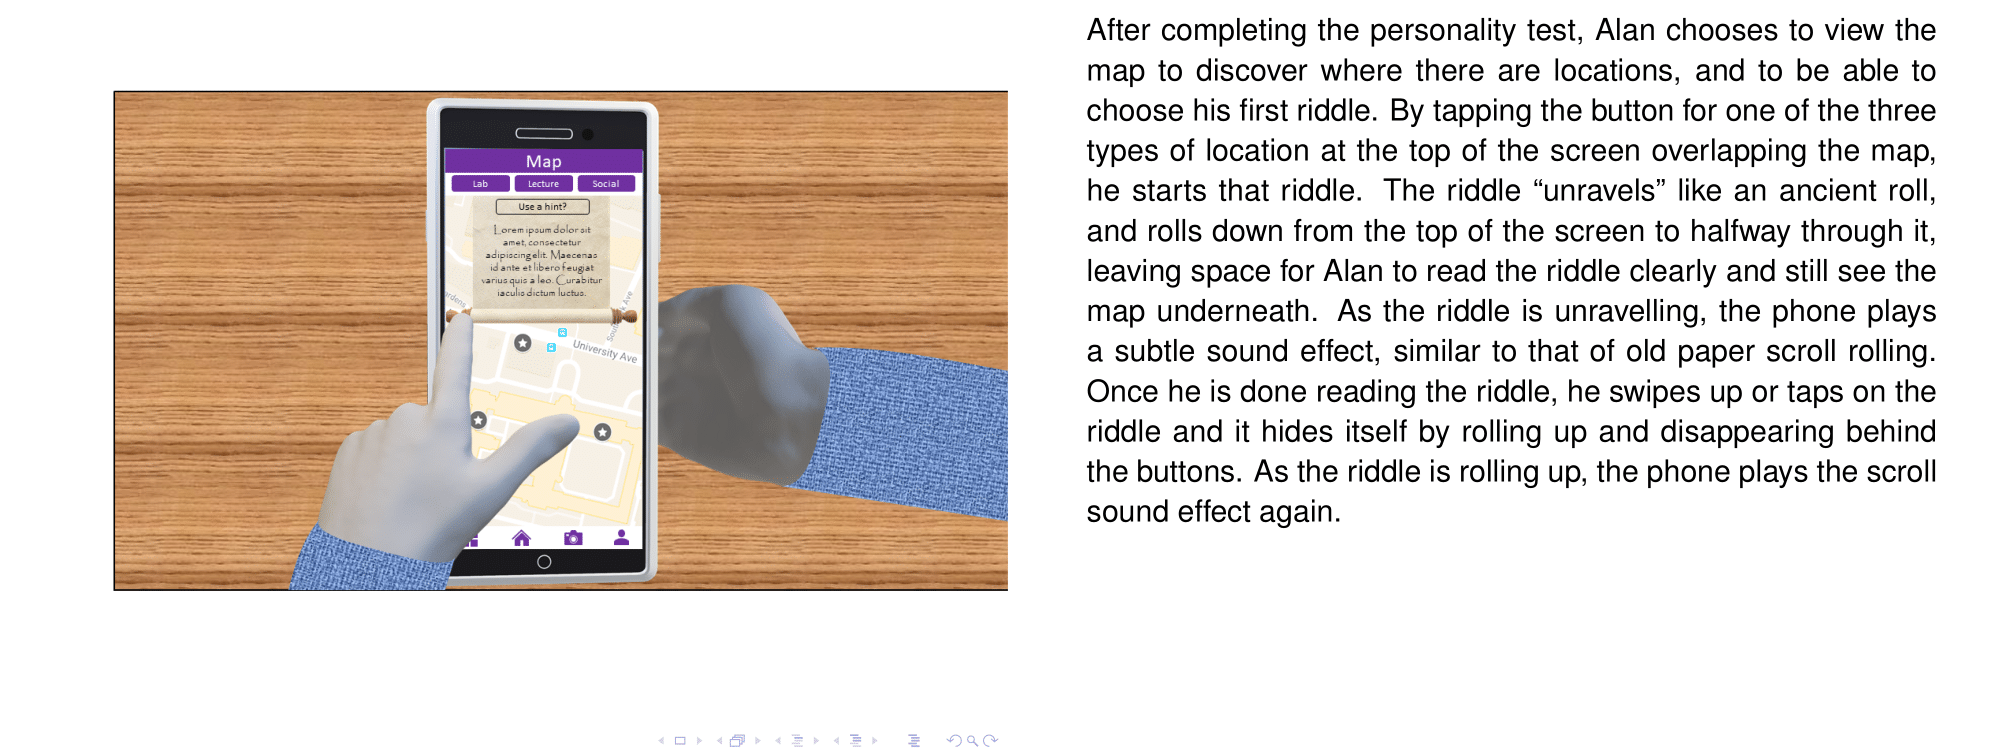
\includegraphics[width=\paperwidth]{./figures/finalStoryboards/finalStoryboards-1.png}}
\end{center}
\begin{center}
  \noindent\makebox[\textwidth]{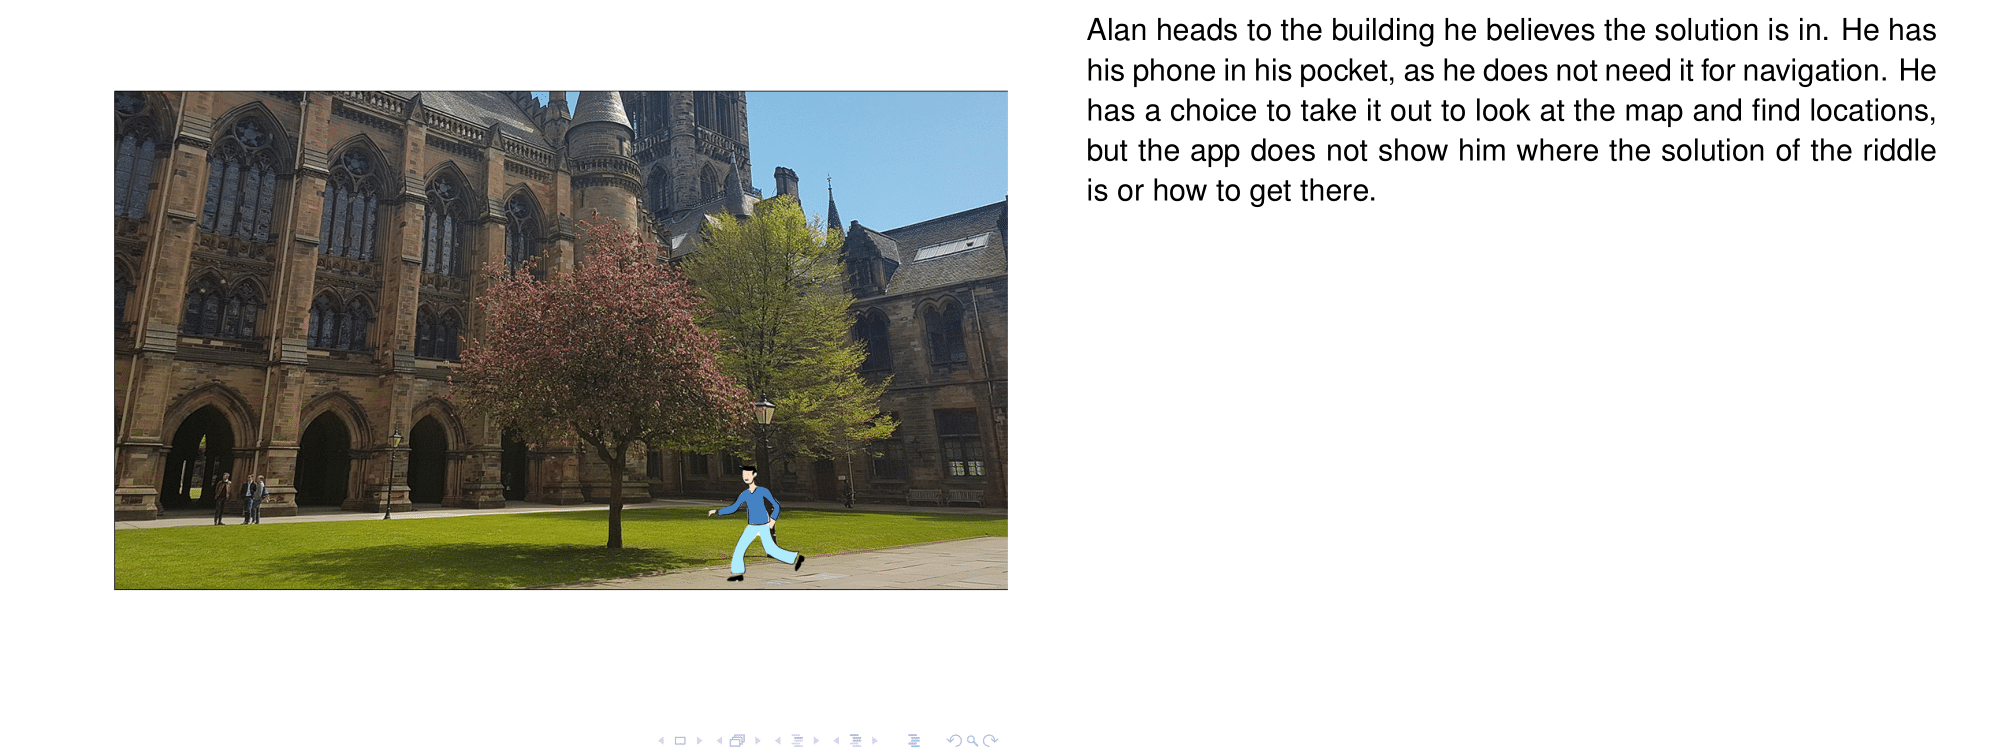
\includegraphics[width=\paperwidth]{./figures/finalStoryboards/finalStoryboards-2.png}}
\end{center}
\begin{center}
  \noindent\makebox[\textwidth]{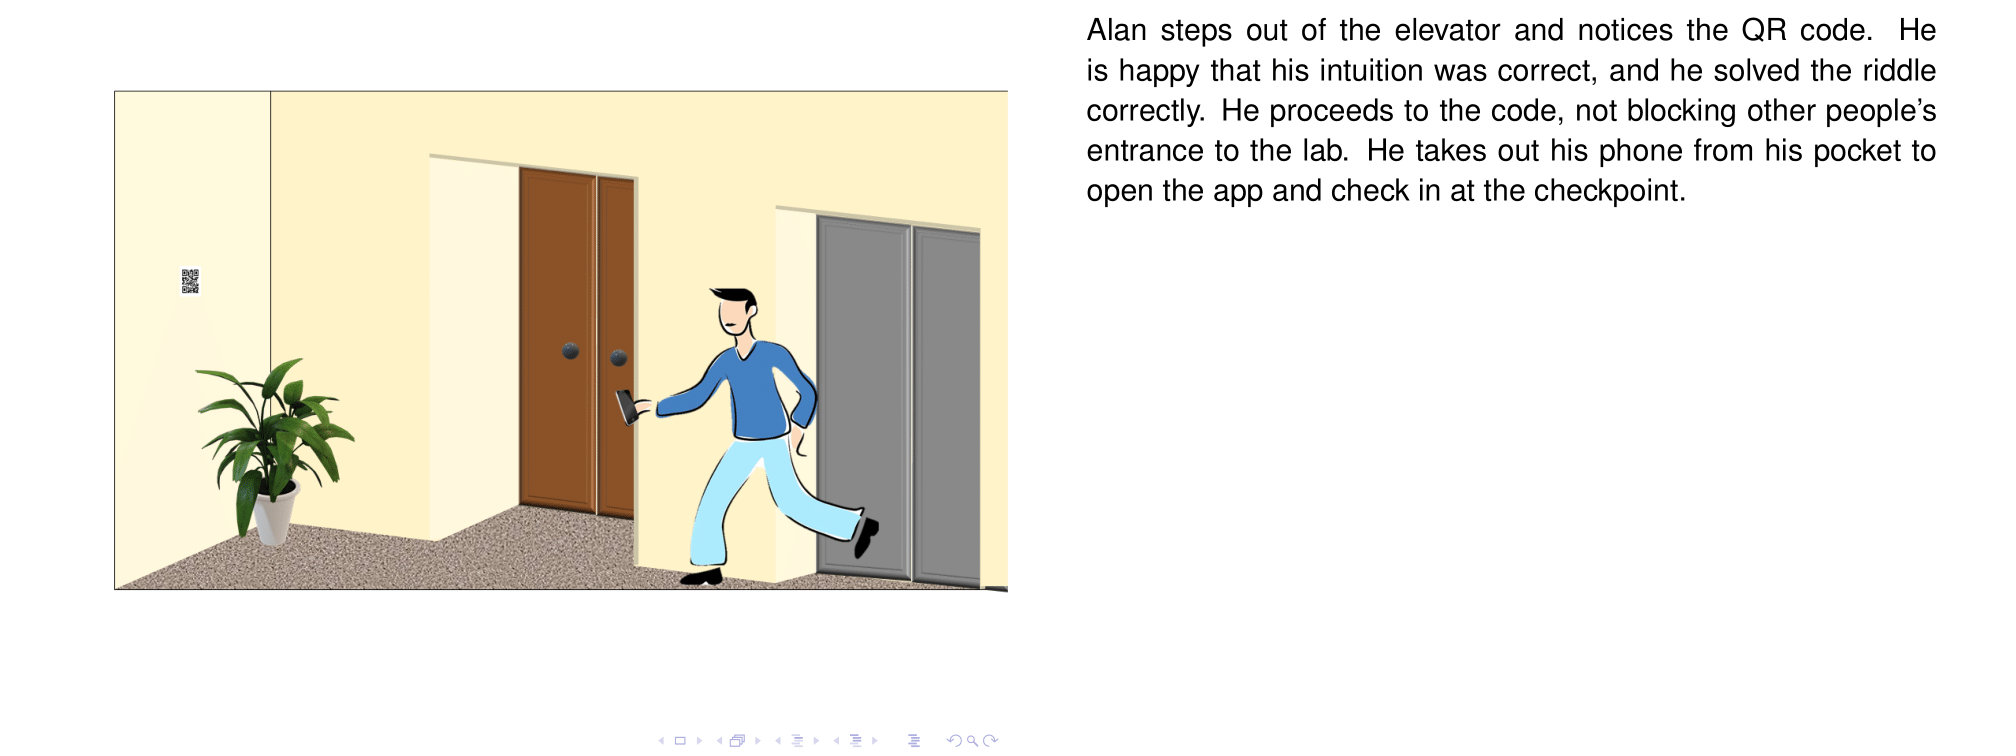
\includegraphics[width=\paperwidth]{./figures/finalStoryboards/finalStoryboards-3.png}}
\end{center}
\begin{center}
  \noindent\makebox[\textwidth]{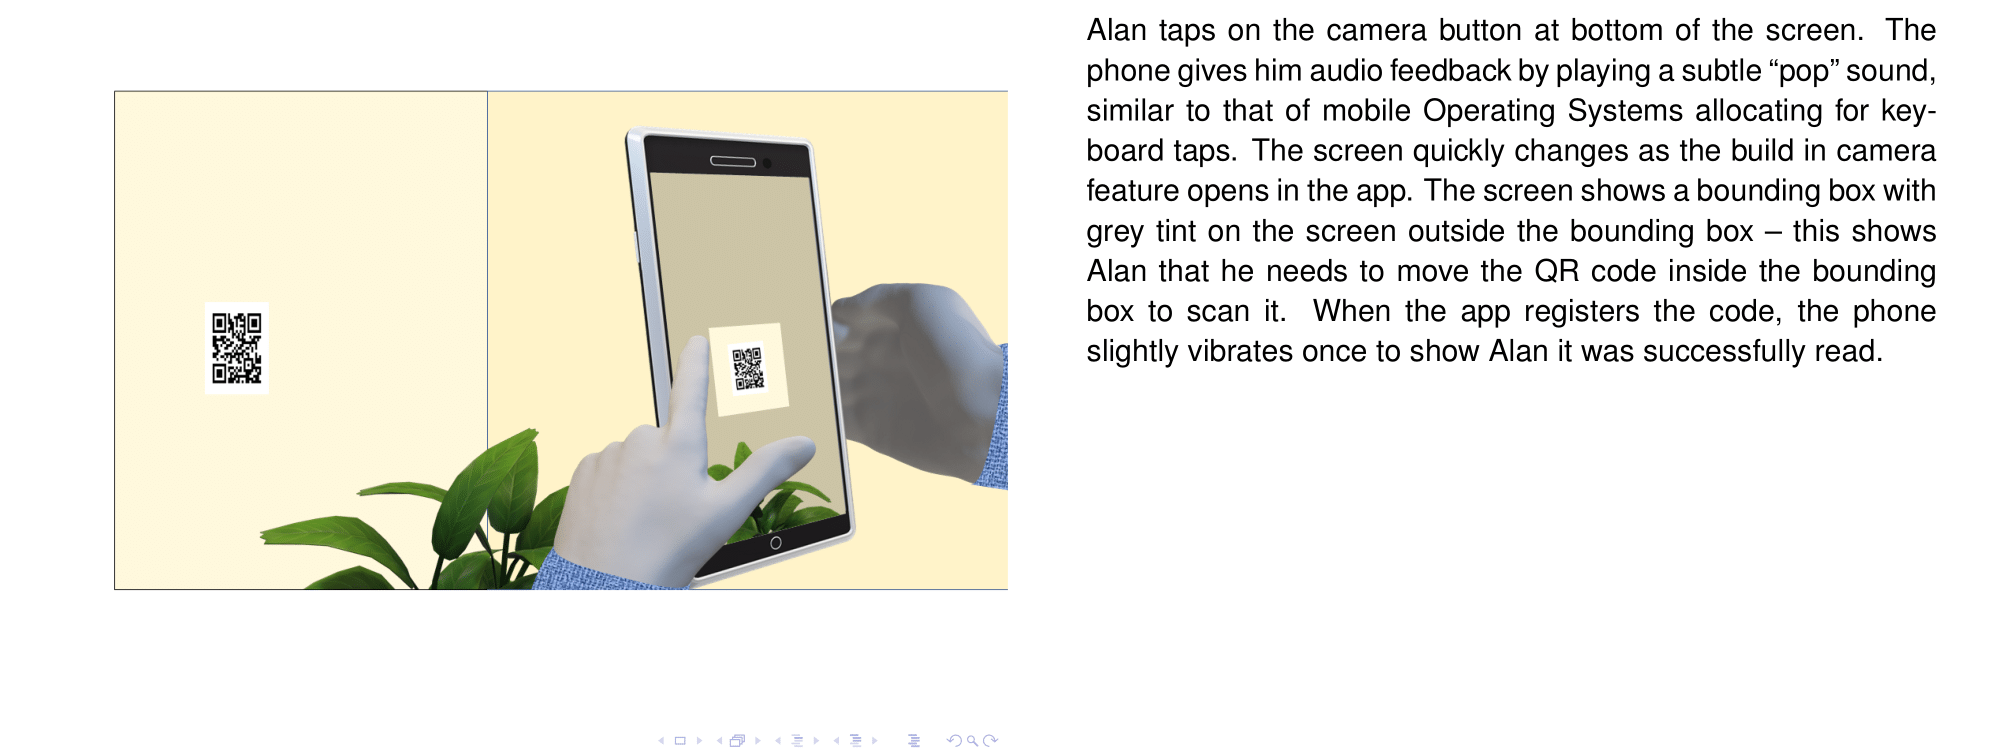
\includegraphics[width=\paperwidth]{./figures/finalStoryboards/finalStoryboards-4.png}}
\end{center}
\begin{center}
  \noindent\makebox[\textwidth]{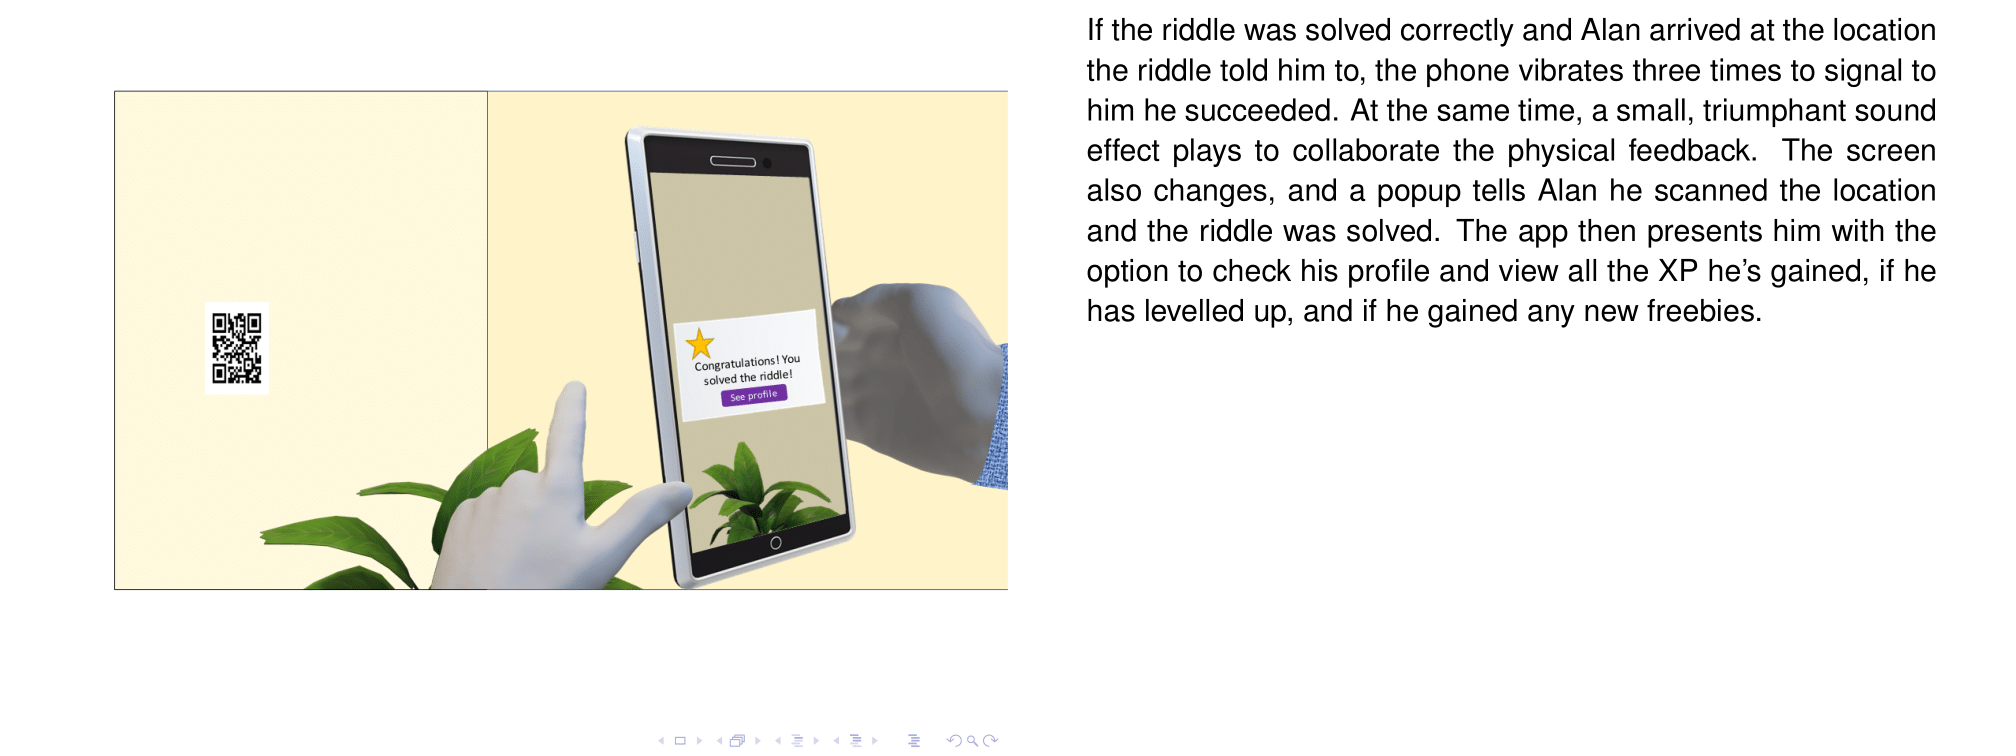
\includegraphics[width=\paperwidth]{./figures/finalStoryboards/finalStoryboards-5.png}}
\end{center}
\begin{center}
  \noindent\makebox[\textwidth]{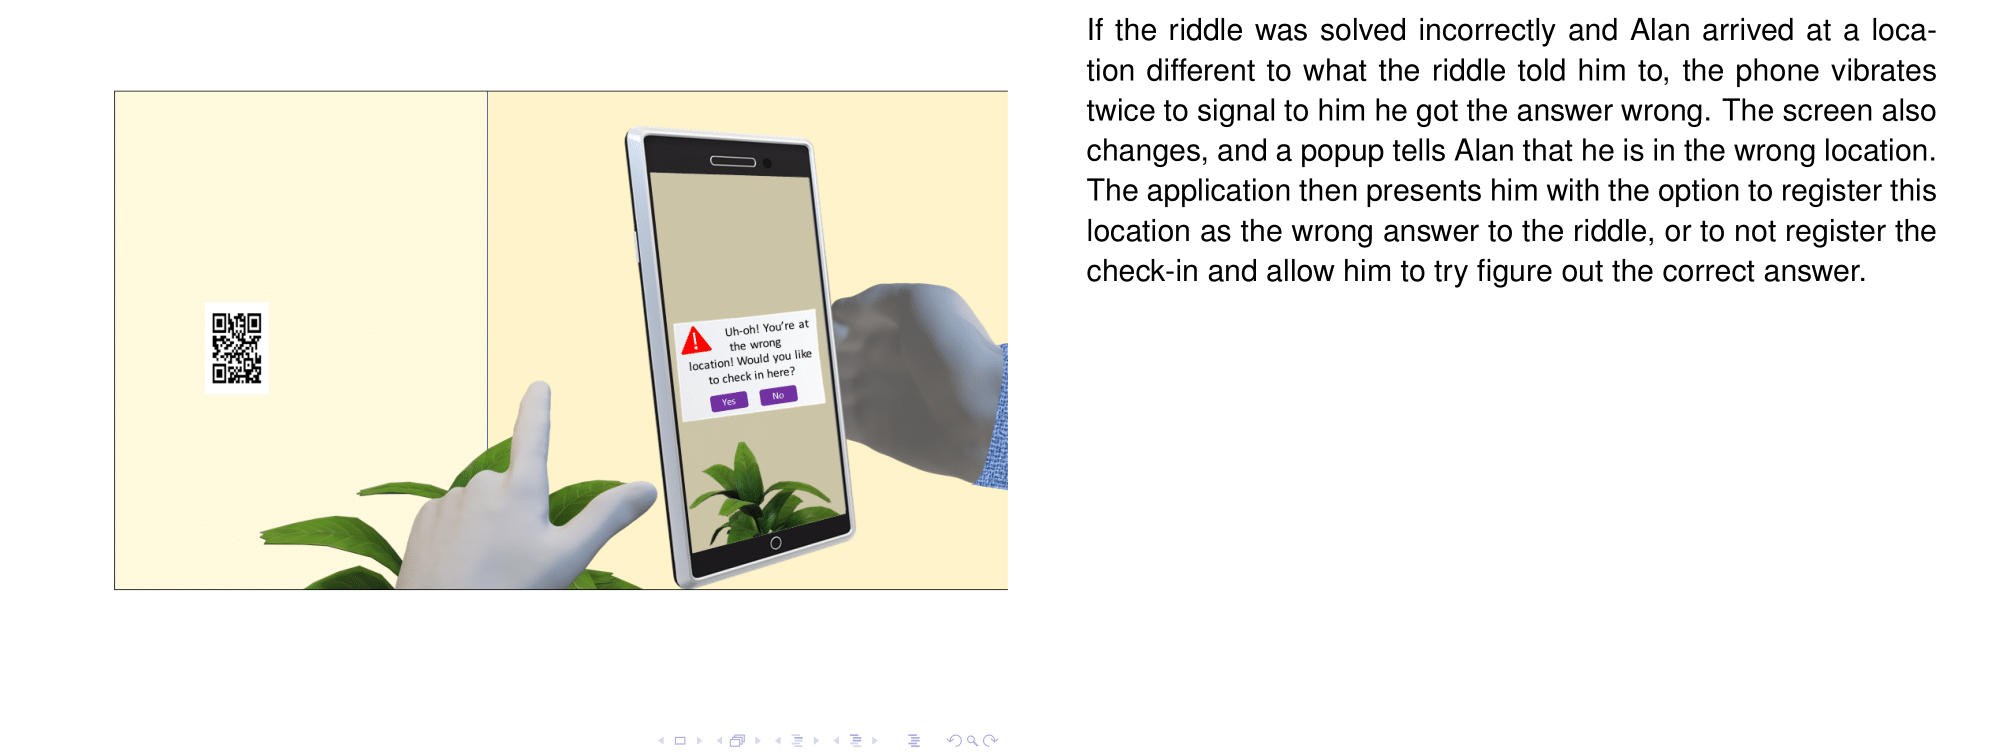
\includegraphics[width=\paperwidth]{./figures/finalStoryboards/finalStoryboards-6.png}}
\end{center}
\begin{center}
  \noindent\makebox[\textwidth]{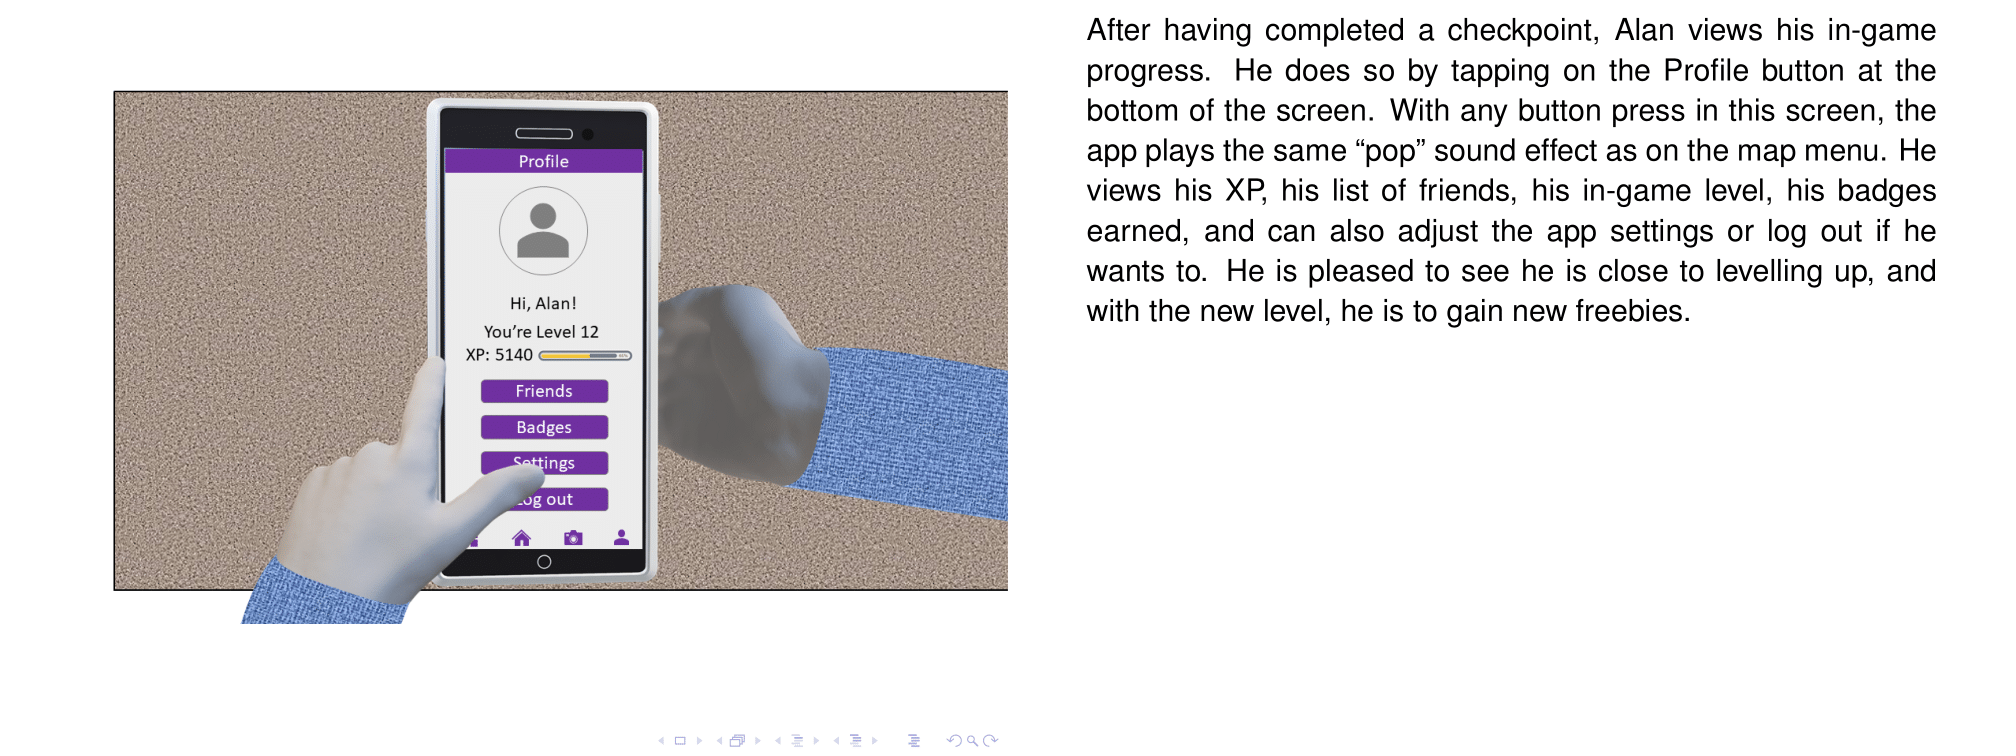
\includegraphics[width=\paperwidth]{./figures/finalStoryboards/finalStoryboards-7.png}}
\end{center}
\begin{center}
  \noindent\makebox[\textwidth]{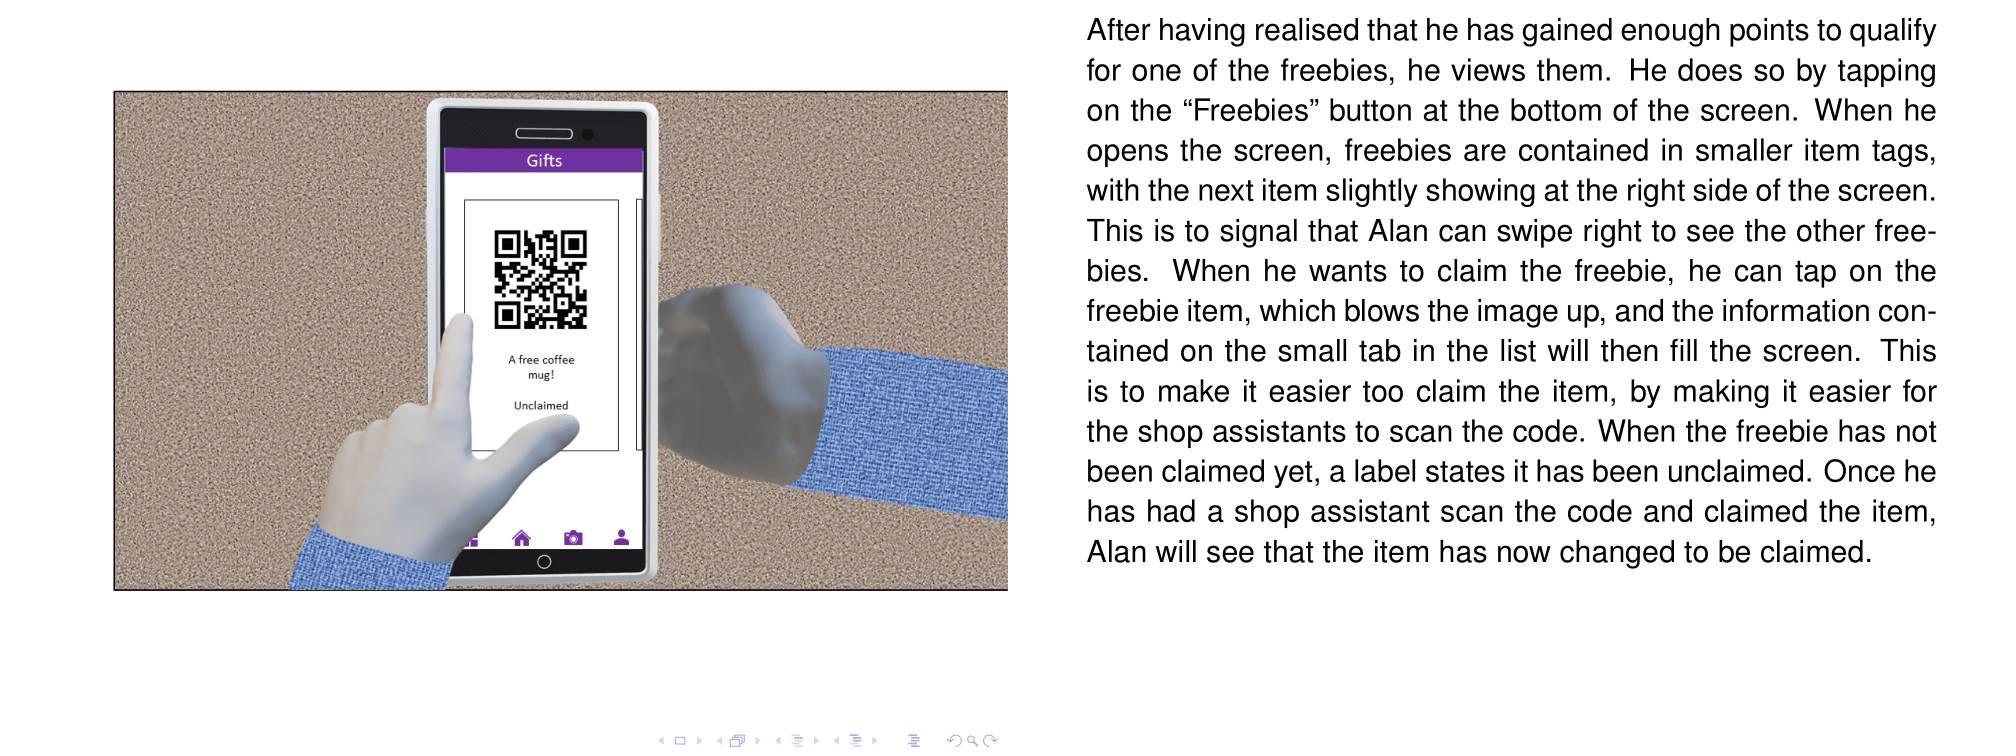
\includegraphics[width=\paperwidth]{./figures/finalStoryboards/finalStoryboards-8.png}}
\end{center}


\end{document}
